\documentclass[11pt,onecolumn]{article} % one column

% !TEX root = NSF_SuperCDMS_SNOLAB_OPS.tex
%--------------------------------------------------------------------
%--------------------------------------------------------------------

%%% PACKAGES

%--------------------------------------------------------------------
%--------------------------------------------------------------------

%%% PDF related packages
%\usepackage{lineno}
%\linenumbers
\usepackage{ifpdf} 
\ifpdf % PDF-specific preamble
\usepackage[pdftex,margin=1in]{geometry} % Use the showframe option to draw a ``margin'' box
%\usepackage{showframe}
\usepackage[pdftex]{graphicx}
\usepackage[pdftex]{xcolor} % color or xcolor?
\usepackage[pdftex,colorlinks,urlcolor=blue,linkcolor=blue,citecolor=red,pdfstartview=FitH]{hyperref} %turn this on for clickable PDF files:
%%\pdfinfo{
%%    /Title  (SuperCDMS Base Funding Proposal)
%%    /Author (Tarek Saab)
%%    /Keywords(Saab,Tarek,SuperCDMS)}
\tolerance=600 %\hypersetup{pdfpagemode=UseThumbs}

\else % preamble for LaTeX

\usepackage[dvips]{geometry}
\usepackage[dvips]{color}
\usepackage[dvips,backref]{hyperref}
\fi

\usepackage[final]{pdfpages} %%% Allows you to include pdf files

%----------------------------------------------------------------------
%----------------------------------------------------------------------

%%% Mathematical symbols, figures, floats, etc ...

\usepackage{amssymb}
\usepackage{amsmath}

\usepackage{xspace} %\xspace saves the user from having to type \? or {} after most occurrences of a macro name in text.
\usepackage{isotope} 
%\renewcommand{\isotopestyle}{\sf} 

%\usepackage{subfigure} % make it possible to include more than one captioned figure/table in a single float
\usepackage{wrapfig}
%\usepackage{booktabs} % for much better looking tables
%\usepackage{multirow}
%\usepackage{array} % for better arrays (eg matrices) in maths

%----------------------------------------------------------------------
%----------------------------------------------------------------------

%%% Misc
%\usepackage[light]{draftcopy}

%----------------------------------------------------------------------
%----------------------------------------------------------------------

%%% Appearance

\usepackage{setspace}
\setstretch{1.0}


%%%%%%Call currvita to define the cv environment
%\usepackage[ManyBibs,NoDate]{currvita}
%
%%Define sans serif fonts for headings
%\renewcommand*{\cvheadingfont}{\Large\bfseries\sffamily}
%%\renewcommand*{\cvlistheadingfont}{\large\bfseries\sffamily}
%\renewcommand*{\cvlistheadingfont}{\large\sffamily}

%%\usepackage{bibunits}
%%\usepackage[english]{babel}
\usepackage{paralist} % very flexible & customisable lists (eg. enumerate/itemize, etc.)
%%%%%% These packages are all incorporated in the memoir class to one degree or another...

%%% Pick your font:
%\usepackage{times}
%\usepackage{charter}
%\usepackage{helvet}
%\usepackage{palatino}

%--------------------------------------------------------------------
%--------------------------------------------------------------------

%%% HEADERS & FOOTERS
\usepackage{fancyhdr}
\usepackage[small,compact]{titlesec}
\pagestyle{fancyplain}
\lhead{}
\cfoot{}
\rfoot{\thepage}
\renewcommand{\headrulewidth}{0pt}

%--------------------------------------------------------------------
%--------------------------------------------------------------------

% See the ``Article customize'' template for come common customizations

%%% SECTION TITLE APPEARANCE
%\usepackage[small,compact]{titlesec}   %%%% title sec doesn't play nice with sectsty, i.e. it overrides the all sections font setting. (it it is placed after)

%%\usepackage{sectsty}
%%\allsectionsfont{\sffamily\mdseries\upshape} % (See the fntguide.pdf for font help)

%% chapters, sections, and subsections will have numbers but not subsubsections or below depending on the numerical value
\setcounter{secnumdepth}{3}


%----- Heidi's section macros (From Tali's NU template)
%\newcommand{\mysection}[1]{{\vskip 0 pt \noindent \bf \Large #1\\ \vskip -17 pt }}
\newcommand{\mysection}[1]{{\vskip 0 pt \noindent \bf \large #1\\ \vskip -15 pt }}
\newcommand{\mysubsection}[1]{{\noindent\bf\large #1 \\\vskip -15 pt}}
\newcommand{\mysubsubsection}[1]{{\noindent\bf\em #1}}

% Setting the inter-paragraphs and indent spacing.
\parskip 0 pt
\parindent 20 pt

%--------------------


%%%% ToC APPEARANCE
%\usepackage[none]{tocbibind} % Put the bibliography in the ToC, ... not with the ``none'' options selected.

%%% Can't get this to work with subfigure. Must find out why ???
%\usepackage[titles,subfigure]{tocloft} % Alter the style of the Table of Contents
%\renewcommand{\cftsecfont}{\rmfamily\mdseries\upshape}
%\renewcommand{\cftsecpagefont}{\rmfamily\mdseries\upshape} % No bold!

%%% Float captions and making captions tighter
\usepackage[font={small,sf},labelfont=bf]{caption} % Manipulate caption fonts, make captions smaller, etc...
\renewcommand\floatpagefraction{.8}
\renewcommand\topfraction{.8}
\renewcommand\bottomfraction{.8}
\renewcommand\textfraction{.2}
% and to pack the captions a bit tighter
\floatsep = 10pt  		%separation between floats
%\intextsep=-2pt		%space above and below in-text floats
\abovecaptionskip = 5pt 	%space above caption
\belowcaptionskip = 5pt	%space below caption
\dbltextfloatsep = 0pt 	%space between figure at top of column and text

%----------------------------------------------------------------------
%----------------------------------------------------------------------

%%% If you feel like playing with page layout sizes:
%%\textwidth = 6.5 in
%%\textheight = 8.5 in
%%\textheight = 11 in
%%\addtolength\headsep{0in}
%%%\headsep = 0.5in
%%\addtolength\textheight{-2in}
%%%\addtolength\textheight{-\footskip}
%%\addtolength\textheight{-\headsep}
%%\oddsidemargin =  0.0 in

%----------------------------------------------------------------------
%----------------------------------------------------------------------

%%Define line for front page / appendices
\newcommand{\Line}[0]{
\vspace{-20pt}    %%% this value depends on using the \allsectionsfont{\sffamily\mdseries\upshape}  in sectsty.
\rule{0pt}{0pt}\hrule\rule{0pt}{0pt}
%\vspace{-6pt}
}

%----------------------------------------------------------------------
%----------------------------------------------------------------------

\newcommand{\SkipSection}[2]{
	\ifnum #1 = 1
		% do nothing
	\else 
		% pass on the second argument as is
		#2
	\fi
}


%--------------------------------------------------------------------
%--------------------------------------------------------------------
%!TEX root = NSF_2016_Northwestern_Base.tex

%Editting Comments
% Comments are set to do nothing to produce a passable Project Summary for the Denver Submission.
\newcommand{\comment}[1]{{\color{red} \bf{#1}}}
%\newcommand{\comment}[1]{}

\def\tali#1{{\bf  \textcolor{purple}{[EFF: {#1}]}}}



\def\MP#1{{\bf  \textcolor{magenta}{[MP: {#1}]}}}
%\def\MP#1{{{}}}



% Text shortcuts/definitions
%\newcommand{\ZIP}{{\small ZIP}}
%\newcommand{\TES}{{\small TES}}\newcommand{\SQUID}{{\small SQUID}}
%%\newcommand{\scdmsSoudan}{\mbox{SuperCDMS at Soudan}\xspace}
%%\newcommand{\scdms}{\mbox{SuperCDMS}\xspace}
%\newcommand{\geant}{\mbox{Geant~4}\xspace}
%\newcommand{\cevns}{\mbox{CE$\nu$NS}\xspace} 
%\newcommand{\EDELWEISS}{{\small EDELWEISS}\xspace}

% Hyphenations
\hyphenation{Ca-lo-ri-me-ter}
\hyphenation{mi-cro-ca-lo-ri-me-ter}
\hyphenation{mi-cro-ca-lo-ri-me-ters}

% Journals
\def\prd{Physical Review D} 
\def\apjl{Astrophysical Journal} 
\def\aap{Astronomy and Astrophysics} 


% Institutions
\newcommand{\DOE}{{\small DOE}}
\newcommand{\UCD}{{\small UCD}}
\newcommand{\SLAC}{{\small SLAC}}
\newcommand{\NIST}{{\small NIST}}
\newcommand{\Minnesota}{{\small U. Minnesota}}
\newcommand{\UCB}{{\small UCB}}
\newcommand{\UMN}{{\small UMN}}
\newcommand{\CWRU}{{\small CWRU}}
\newcommand{\UF}{\mbox{\small U. Florida}\xspace}
\newcommand{\MIT}{\mbox{\small M.I.T.}\xspace}
\newcommand{\UCBB}{{\small U.C.~Berkeley}\xspace}
\newcommand{\TAMU}{{\small Texas A\&M University}\xspace}


% Experiments
\newcommand{\CDMS}{{\small CDMS}\xspace}
\newcommand{\CDMSI}{{\small CDMS\,I}\xspace}
\newcommand{\CDMSII}{{\small CDMS\,II}\xspace}
\newcommand{\SuperCDMS}{{\small SuperCDMS}\xspace}
\newcommand{\scdmssnolab}{{\small SuperCDMS SNOLAB}\xspace}
\newcommand{\scs}{{\small SuperCDMS SNOLAB}\xspace}
\newcommand{\SNOLAB}{{\small SNOLAB}\xspace}
\newcommand{\Soudan}{{\small Soudan}\xspace}
\newcommand{\DAMIC}{{\small DAMIC}\xspace}
\newcommand{\EDELWEISS}{{\small EDELWEISS}\xspace}
\newcommand{\antonella}{{\small ANTONELLA}\xspace}

% Misc
\newcommand{\WIMP}{{\small WIMP}\xspace}
\newcommand{\WIMPs}{{\small WIMP}s}
\newcommand{\RnD}{{\small R\&D}}
\newcommand{\ZIP}{{\small ZIP}}
\newcommand{\TES}{{\small TES}}
\newcommand{\DCRC}{{\small DCRC}}
\newcommand{\SQUID}{{\small SQUID}}
\newcommand{\SQUIDs}{{\small SQUID}s}
\newcommand{\JFET}{{\small JFET}}
\newcommand{\JFETs}{{\small JFET}s}
\newcommand{\LED}{{\small LED}}
\newcommand{\LEDs}{{\small LED}s}
\newcommand{\HEMT}{{\small HEMT}}
\newcommand{\HEMTs}{{\small HEMT}s}
\newcommand{\RFQ}{{\small RFQ}}
\newcommand{\RFQs}{{\small RFQ}s}
\newcommand{\WBS}{{\small WBS}\xspace}
\newcommand{\cevns}{{\small CE$\nu$NS}\xspace}


% Facilities
\newcommand{\cute}{{\small CUTE}\xspace}
\newcommand{\nexus}{{\small NEXUS}\xspace}
\newcommand{\minos}{{\small MINOS}\xspace}
\newcommand{\numi}{{\small NuMI}\xspace}
\newcommand{\tunl}{{\small TUNL}\xspace}

% Units

\newcommand{\evee}{\ensuremath{\textrm{eV}_\textrm{ee}}} %ev ee
\newcommand{\eVee}{\ensuremath{\textrm{eV}_\textrm{ee}}} %ev ee
\newcommand{\evr}{\ensuremath{\textrm{eV}_\textrm{r}}} % ev recoil units for event rates
\newcommand{\eVr}{\ensuremath{\textrm{eV}_\textrm{r}}} % ev recoil units for event rates
\newcommand{\keVee}{\ensuremath{\textrm{keV}_\textrm{ee}}} % keV ee
\newcommand{\keVr}{\ensuremath{\textrm{keV}_\textrm{r}}} % keV recoil Units for event rates
\newcommand{\keVvis}{\ensuremath{\textrm{keV}_\textrm{vis}}} % keV visible - some 
\newcommand{\evt}{\ensuremath{\textrm{eV}_\textrm{t}}}


\newcommand{\perkkd}{/keV/kg/day} % /keV/kg/day
\newcommand{\perkky}{/keV/kg/year}
\newcommand{\perkgd}{/kg/day} % /kg/day
%%% redundant definition
\newcommand{\kgd}{kg--day} % /kg/day
\newcommand{\perhkgy}{/100~kg/year} % /100kg/year
\newcommand{\kgdnet}{\ensuremath{\textrm{net kg--days}}} % /kg/days

\newcommand{\etal}{et al.}   			% et al in appropriate format, the following . 
\newcommand{\pl}{{\it Phys. Lett. }} 		% Physics Letters, note space at end

\newcommand{\mus}{\ensuremath{\mu{}s}} % micro-secs
\newcommand{\mwe}{mwe} % mwe
\newcommand{\lapprox}{\ensuremath{\lesssim}}
\newcommand{\gapprox}{\ensuremath{\gtrsim}}
\newcommand{\micron}{\ensuremath{\mu \textrm{m}}} % um

\newcommand{\kg}{\ensuremath{\,\mathrm{kg}}\xspace}
\newcommand{\mm}{\ensuremath{\,\mathrm{mm}}\xspace}
\newcommand{\cm}{\ensuremath{\,\mathrm{cm}}\xspace}
\newcommand{\um}{\ensuremath{\,\mu\mathrm{m}}\xspace}
\newcommand{\ms}{\ensuremath{\,\mathrm{ms}}\xspace} % milli-secs
\newcommand{\us}{\ensuremath{\,\mu\mathrm{s}}\xspace} % micro-secs
\newcommand{\Hz}{\ensuremath{\,\mathrm{Hz}}\xspace} % Hz
%

\newcommand{\mwimp}{m_\chi\xspace}
\def\mnucl{m_{N}}
\def\redN{\mu_N}
\def\redN{\mu_N}
\def\sigmaN{\sigma_{WN}}
\def\sigmaNsi{\sigma_{WN}^{SI}}
\def\sigmaNsd{\sigma_{WN}^{SD}}
\newcommand{\mchi}{m_{\chi}}
\newcommand{\sigsi}{\sigma^{SI}}
\newcommand{\sigsd}{\sigma^{SD}}
\newcommand{\sigsip}{\sigma^{SI}_{p}}
\newcommand{\sigsin}{\sigma^{SI}_{n}}
\newcommand{\sigsdp}{\sigma^{SD}_{p}}
\newcommand{\sigsdn}{\sigma^{SD}_{n}}
\newcommand{\svave}{\langle\sigma v\rangle}
\newcommand{\sv}{(\sigma v)}
\newcommand{\Sp}{\langle S_p \rangle}
\newcommand{\Sn}{\langle S_n \rangle}

\def\gev{GeV/c$^2$\xspace}
\def\mev{MeV/c$^2$\xspace}
\def\cm2{cm$^2$\xspace}

% Unit shortcuts
\renewcommand{\deg}{\ensuremath{{^\circ}}\xspace}
\newcommand{\mK}{\ensuremath{\,\mathrm{mK}}\xspace}
%
\newcommand{\volt}{\ensuremath{\,\mathrm{V}}\xspace} 
\newcommand{\eV}{\ensuremath{\,\mathrm{eV}}\xspace}
\newcommand{\keV}{\ensuremath{\,\mathrm{keV}}\xspace}
\newcommand{\MeV}{\ensuremath{\,\mathrm{MeV}}\xspace}
\newcommand{\GeVcc}{\ensuremath{\,\mathrm{GeV}/\mathrm{c}^2}\xspace}
%
%\newcommand{\perkkd}{/keV/kg/day\xspace} % /keV/kg/day
%\newcommand{\perkgd}{/kg/day\xspace} % /kg/day
%\newcommand{\perhkgy}{/100~kg/year\xspace} % /100kg/year
%\newcommand{\kgd}{kg--day\xspace} % /kg/day
%\newcommand{\mwe}{mwe\xspace} % mwe
%%
%\newcommand{\mwimp}{m_\chi\xspace}
%
%\newcommand{\kg}{\ensuremath{\,\mathrm{kg}}\xspace}
%\newcommand{\mm}{\ensuremath{\,\mathrm{mm}}\xspace}
%\newcommand{\cm}{\ensuremath{\,\mathrm{cm}}\xspace}

%\newcommand{\um}{\ensuremath{\,\mu\mathrm{m}} \xspace}
%\newcommand{\ms}{\ensuremath{\,\mathrm{ms}}\xspace} % milli-secs
%\newcommand{\us}{\ensuremath{\,\mu\mathrm{s}}\xspace} % micro-secs
%\newcommand{\Hz}{\ensuremath{\,\mathrm{Hz}}\xspace} % Hz
%%


% Added by Ben
\newcommand{\E}[1]{$\times10^{#1}$}

\newcommand{\iso}[2]{$^{#2}$#1\xspace}
\newcommand{\Pb}[1][210]{\iso{Pb}{#1}}
\newcommand{\Bi}[1][210]{\iso{Bi}{#1}}
\newcommand{\U}[1][238]{\iso{U}{#1}}
\newcommand{\Th}[1][232]{\iso{Th}{#1}}
\newcommand{\K}[1][40]{\iso{K}{#1}}

\newcommand{\Ba}{\isotope[133]{Ba}\xspace}

%%%% redundant commands
\def\8B{$^8$B\xspace}
\def\206pb{$^{206}$Pb\xspace}	
\def\210pb{$^{210}$Pb\xspace}
\def\210bi{$^{210}$Bi\xspace}
\def\235u{$^{235}$U\xspace}
\def\um{$\mu$m}

\newcommand{\geant}{\texttt{GEANT4}\xspace}
\newcommand{\sources}{\texttt{SOURCES4a}}
\newcommand{\alphan}{($\alpha$,n)}

\begin{document}
\onecolumn

\begin{titlepage}

\begin{center}
\textbf{\Huge Collaborative Research:}\\[0.9cm]
\textbf{\Huge The SuperCDMS SNOLAB}\\[0.8cm]
\textbf{\Huge Experiment}\\[1.8cm]

\begin{figure}
\begin{center}

\includegraphics[height=1in]{Figures/SuperCDMS_logo.png}
\end{center}
\end{figure}

\textrm{\today}\\[1.8cm]

\textrm{\LARGE The NSF Members of the SuperCDMS Collaboration}\\[0.9cm]
\textit{\Large
Northwestern University \\
South Dakota School of Mines and Technology \\
Southern Methodist University \\
University of California at Berkeley \\ 
University of Colorado Denver \\
University of Florida \\} 

\end{center}


\end{titlepage}
\clearpage

%!TEX root = NSF_SuperCDMS_SNOLAB_OPS.tex

\pagenumbering{gobble}
\lhead{\Large\bf Project Summary} 

\begin{center}
{\large{\bf Elements: Improving tools based on data-description standards for gigabyte-scale data sets}}
\end{center}

{\bf Overview:} The long-term goal of this work is to build and create community buy-in for a set of tools for the nuclear physics community to access binary data.  The intent is to address one piece of a common software need in the community that is repeatedly solved in isolation and that costs the entire community unnecessary time and limits access to data and science. In pursuit of this goal, this proposal has four objectives:  
(1) Define a data-description language that allows scientists to describe any binary data format.
(2) Improve existing software that automatically builds a convenient data-access library for any user-described data so that it works well with gigabyte-scale datasets.
(3) Build community and support adoption of these community tools.
(4) Increase access to analysis of original scientific data sets for undergraduate students, graduate students and postdocs, early career researchers, and scientists whose labs do not have access to dedicated software support. 
These objectives will be met as follows:

{\it (1) Defining a data-description standard:} The PI will use two already-existing standards that both have broad user support, DFDL and Kaitai-Struct.  Kaitai-Struct will be used and where necessary further defined as the software created around this standard is better-suited to the needs of data analysis.

{\it (2) Improving standards-based analysis software:} Scientists who wish to generate a convenient library that allows them to read custom-format data can already do so using the existing Kaitai software.  However, this software has poor performance in python for files larger than a gigabyte and this significantly limits the usefulness of this software to the nuclear physics community, particularly as data acquisition systems move to storing digitized pulses rather than pre-processed data.  The PI proposes to create another Kaitai target that allows scientists to auto-generate a library that targets the awkward-array interface built and maintained by the IRIS-HEP collaboration.  This data structure is designed to give rapid data-analysis access to the high energy physics community and is routinely tested on data sets that exceed several hundred gigabytes.

{\it (3) Building community:} The PI proposes to hold yearly workshops to bring together developers and scientists for training, user feedback, and software development.  In addition, the PI has requested funds for graduate and undergraduate stipends and travel awards to foster community participation.

{\it (4) Increasing Access:} Many students who have the interest and ability to participate in science analysis are blocked by a lack of training in scientific computing.  The often-complex scientific computing ecosystem is poorly represented in most physics curriculum and even computer science courses do not usually prepare students for the variety of systems they need to navigate to do typical data analysis.  The PI requests funding for undergraduate students to develop and test documentation and training materials for fundamental scientific computing concepts and skills in addition to testing the documentation for the standards-based analysis tools.

\textbf{Intellectual merit}: This grant supports the science effort of a dark matter experiment, the SuperCDMS experiment, and the broader nuclear physics community that is in need of software support.  At present this includes scientists working on the origin of the elements in the universe, fundamental symmetry testing, and detector testing for improved threat detection.

\textbf{Broader impacts}: The PI proposes this work because it would be immediately useful to her dark matter work and because software supported by an entire community that can provide easy access to any data format would meet an increasingly-urgent need of communities dealing with gigabyte-scale data.

Focusing previously-isolated software efforts on a community solution offers the benefit of software that is well-tested and well-documented and with a community that can provide support for its users.

With materials available to help students and new researchers learn the basic skills required for science analysis, students can begin participating in true science research at much earlier stages, with less reliance on patient, local expertise being available at their institution.  Right now, real science analysis is at best painfully accessible to a narrow set of students.  With a small set of community standards and tools, we can broaden science access to a much wider group of individuals and increase the time expert scientists can spend on actual science.


\clearpage
\lhead{}

\tableofcontents
\clearpage

\setcounter{tocdepth}{2}
\pagenumbering{arabic}

% !TEX root = NSF_SuperCDMS_SNOLAB_OPS.tex

\section{Introduction (1 page)}\label{sec:overview}
\tali{A lot of this text may not be needed as it mirrors the 1-page summary}
The long-term goal of the \scs collaboration is to improve the understanding of dark matter by answering the following questions: what are its constituents, what are their particle and astrophysical properties, and how do they relate to the Standard Model? In pursuit of this goal, this proposal has four objectives:  
(1) Perform necessary calibration and performance measurements of \scs detectors to maximize the science return from the experiment.
(2) Commission and operate the \scs experiment.
(3) Measure a dark matter signal or place world-leading limits for the dark matter--nucleon cross section at masses below 10~\gev.
(4) Train the next generation of scientists through research and outreach activities, and teach secondary students and the public about dark matter science. 
These objectives will be met as follows:

%\comment{Possible rewording for here and the overview page: (3) Train the next generation of scientists to be teacher scholars through engaging them in teaching secondary students and the public about dark matter science. - Joel}
%$\bullet$
%{\it Detector Calibration:} A calibration of the nuclear recoil energy scale is required in order to produce scientific results from the data from \scs. This proposal outlines a calibration measurement campaign which includes high-precision measurements at a neutron beam facility and pre-production \scs detector measurements with a D--D neutron generator at the low-background NEXUS facility located at Fermilab.
 
%{\it Performance and Backgrounds Measurements:} Detailed tests of the performance of \SuperCDMS dark matter detectors must be done in an underground low-background facility. This proposal outlines a measurement campaign of both pre-production \scs detectors and the first production \scs towers at the \cute facility in SNOLAB that will verify the performance of the detectors, measure background levels, provide data to optimize operational parameters, and potentially provide a dark matter search with world-leading sensitivity. 

{\it Experiment Characterization and Optimization:} In order to maximize the science output of \scs, detailed understanding of the response of detectors to potential signals and backgrounds is required. Measurements at two underground facilities (\nexus at Fermilab and \cute at SNOLAB) will characterize and calibrate pre-production \scs detectors and the first production \scs towers, with supporting measurements from small devices at university test facilities. This data will allow energy scale calibration, measurements of background levels, understanding of the detailed phonon and electron physics of the detectors, and optimization of \scs operational parameters. 

{\it Commissioning and Operation of \scs:} This proposal will fund the NSF-portion of commissioning the \scs experiment and the first year of science operations.

{\it First \scs Science:} This proposal will perform a dark matter search with  world-leading sensitivity using data taken with one \scs Tower at \cute and with the first data set from the full \scs experiment.

{\it Training and Outreach:} The activities in this proposal provide fertile ground for training of postdoctoral researchers and graduate students from the \SuperCDMS collaboration, and opportunities to share the excitement of science with the general public.

\textbf{Intellectual merit}: This grant supports an experiment that will address one of the most fundamental problems of modern science, the nature of dark matter, in a way complementary to the Large Hadron Collider and indirect detection experiments. The \scs experiment will achieve world-leading sensitivity for dark matter  masses less than 10~\gev.

\textbf{Broader impacts}: The \scs experiment will have a broad impact which extends beyond the search for dark matter. The experiment's phonon-mediated detectors have applications in cosmology, astronomy and industry. This effort will contribute opportunities for training of undergraduate and graduate students and postdoctoral researchers.

SuperCDMS will engage in education and outreach at local institutions and will coordinate our outreach at Soudan, SNOLAB, and SURF to increase the broader impact with focus on secondary education. The grant will support participating in SNOLAB-hosted Teacher Workshops, modifying and providing middle school dark matter education modules to U.S. educators, and maintaining SuperCDMS-related outreach materials for SNOLAB, Soudan, and SURF. Existing alliances will enable outreach to Sudbury First Nations communities. This effort will also support post-graduate education by providing speakers for Colegio de F\'{i}sica Fundamental e Interdiciplinaria de las \'{A}mericas summer school in Puerto Rico.

\comment{This paragraph needs updating: }The activities in this proposal are fully coordinated with the \SuperCDMS\ collaboration in general, and its DOE and Canadian-supported institutions. This NSF proposals is tightly coordinated with two R\&D proposals titled ``\SuperCDMS R\&D Toward the Neutrino Floor" that have been awarded from the DOE KA23 and KA25 programs by Fermilab and SLAC respectively. This proposal is also coordinated with the DOE \scs Experimental Operations Plan.  

This collaborative proposal subsumes most of the work done by the NSF institutions on \scs. This includes all calibration, characterization, commissioning, operation, analysis, and publication efforts. It also includes support for students, postdocs, and scientists that would have normally been funded through separate ``base'' proposals by each member institution. This support and expertise from university groups will be instrumental in turning the data products from the \scs experiment into fully vetted scientific results and publications. In addition, this proposal provides fertile ground for training graduate students and postdocs through their participation in the data taking and analysis. 

\comment{This paragraph needs to be added after we do decide on the sections} This project description is organized as follows. 
Sections~\ref{sec:introduction}--\ref{sec:snolab} summarize the science and hardware of the \scs experiment. 
Section~\ref{sec:nexuscute} describes the underground facilities to be used in the pre-operations portion of this proposal.
Section~\ref{sec:operations} describes the plan of work of this effort, and Section~\ref{sec:schedule} describes the schedule.
Section~\ref{sec:management} gives an overview of the management for this proposed grant, and Section~\ref{sec:broad} describes the broader impacts of the work.
Finally, Section~\ref{sec:prev-res} summarizes the results from previous support.


\subsection{Introduction}
\label{sec:introduction}

\tali{This should be trimmed and incorporated into either the project overview or the science section}
A critical research area in particle astrophysics is the search for the nature of dark matter. Dark matter, unlike ordinary matter, does not produce electromagnetic radiation and its only observed interaction with ordinary matter thus far has been gravitational. Its existence explains flat rotation curves of spiral galaxies, structure formation and galaxy cluster evolution, and the anisotropy of the cosmic microwave background. These astronomical observations indicate that approximately 85\% of the matter in the universe must be dark matter, but they do not tell us much about its composition. A long-favored hypothesis is that a class of elementary particles generically labeled as WIMPs (Weakly Interacting Massive Particles) constitutes the dark matter. However, an absence of evidence for a heavy mass WIMP at the LHC and in direct detection dark matter experiments has motivated the development of a wide array of alternate theories which predict dark matter particles with masses between 1~MeV--10~GeV. 

Determining the fundamental nature of dark matter is a high priority science objective for the National Science Foundation (NSF) and the DOE Office of High Energy Physics (OHEP). It is also a major focus for science in Canada, with support from the Natural Sciences and Engineering Research Council of Canada (NSERC) and the Canada Foundation for Innovation (CFI). 

The SuperCDMS collaboration has conducted a series of experiments designed to directly detect dark matter in underground laboratories, using ultra-pure germanium (Ge) and silicon (Si) crystals outfitted with ionization and phonon sensors and operated at cryogenic temperatures. For most of the last two decades, CDMS experiments at Stanford and Soudan have provided leading sensitivity to high-mass WIMPs. Recently SuperCDMS has focused on $<$~10~\gev dark matter candidates, where our technology has unique advantages given the low energy thresholds provided by their athermal phonon sensor technology and Luke-Neganov phonon amplification techniques for ionization.

The NSF and DOE have jointly chosen SuperCDMS SNOLAB as the next-generation project to search for low-mass dark matter. The project is going through the DOE Critical Design (CD) review process and is expected to be complete in 2019. Canada is also supporting SuperCDMS SNOLAB via NSERC and CFI funding. The experiment will be located at SNOLAB, in Ontario, Canada, the deepest underground laboratory in North America.

%\clearpage

% !TEX root = NSF_SuperCDMS_SNOLAB_OPS.tex
\section{Science (4 pages)}
\label{sec:science}

\tali{Scrub this to be more focused on sub-10GeV dark matter}
An abundant amount of evidence supports the existence of dark matter at all scales in the Universe~\cite{Ade:2013zuv}. Although its nature is still unknown, particle dark matter provides the clearest evidence for physics beyond the Standard Model of particle physics, and thus its detection and identification constitute one of the greatest challenges of modern physics. Phenomenology at the intersection of particle physics, cosmology, and astrophysics provides a wide spectrum of viable dark matter candidates that exhibit very different properties. For example, their mass can differ by many orders of magnitude, ranging from $10^{-15}$~eV/c$^{2}$ (in the case of hidden photons) to 10$^{16}$ \gev (for Wimpzillas). Also, their interaction with ordinary matter can be purely gravitational (as in the case of gravitinos) or involve a new interaction scale.

One long-standing favored candidate for particle dark matter is the Weakly Interacting Massive Particle (WIMP), a stable particle with weak-scale interactions that is naturally produced in supersymmetric extensions to the standard model that explain the light mass of the Higgs boson ~\cite{Jungman:1995df,Ellis:1983ew,Agashe:2004ci, Servant:2002aq,Cheng:2002ej,Schmaltz:2010ac} and that can be thermally produced in the early universe in the right amount to account for the observed dark matter relic abundance.

In response to the lack of experimental evidence for WIMPs at the LHC or in direct detection experiments, multiple alternative models have recently been developed that have dark matter candidates with masses within the MeV--10 GeV range \cite{Kaplan:92prl, Kaplan:09prd, Graham:12pdu, Falkowski:11jhep, Feng:08prl, Hall:10jhep, Essig:12prd}. Hidden sector super-symmetric dark matter models, for example, have an extremely small coupling to the visible sector, and thus their production in accelerators and their CMB annihilation signature would be suppressed.  The lack of an annihilation signature in the CMB is also quite natural in a broad class of asymmetric dark matter theories where the measured relic density of dark matter is not due to annihilation freeze out, but rather due to an antimatter-matter asymmetry in dark matter production.

%In many of these alternate models, dark matter within the local galactic halo could be detected through through their elastic scattering off nuclei in a terrestrial detector ~\cite{Goodman:1984dc, Gaitskell:2004gd}. The large difference in mass between GeV scale dark matter and the heavy nuclei in detector target materials produces small recoil energies, e.g. 1 GeV/c$^{2}$ dark matter produces  $\sim$30eV$_{r}$ energy in germanium. Recoil energies of this magnitude are well below the trigger threshold of current experiments optimized for high threshold dark matter searches. In addition, the expected dark matter interaction rate is quite low, less than 0.01 event/kg-day ~\cite{Bertone:2004pz, Lewin:1995rx}, much lower than the radioactive background of most materials. Hence, such detectors are housed deep underground for protection from cosmic rays and fabricated using materials with ultra-low radioactivity.

%Hidden sector super-symmetric DM models, for example, have an extremely small coupling to the visible sector which means that accelerator production is highly suppressed and that there is no measurable CMB annhiliation signature since annihilation products have hidden sector properties \cite{Feng:08prl}.  The lack of an annihilation signature in the CMB is also quite natural in a broad class of asymmetric DM theories where the measured relic density of DM is not due to annihilation freeze out, but rather due to an antimatter-matter asymmetry in DM production. In fact, in direct analogy to the WIMP miracle, the measured DM relic density being $\sim$x5 the relic baryonic density is explained by a GeV scale asymmetric DM candidate which is produced by the same physical mechanism that produces the observed baryonic asymmetry. In summary, future light mass dark matter searches are strongly theoretically motivated.

\subsection{Direct Detection of Light-Mass Dark Matter}

Under many of these theoretical models, dark matter within the local galactic halo can be directly probed via their elastic scattering off nuclei in a terrestrial detector~\cite{Goodman:1984dc, Gaitskell:2004gd}. Even with the enhancement due to %simultaneously coherently 
coherent scattering off a large number of nucleons when using high Z targets like germanium, the expected signal rate is quite low, less than 0.01 event/kg-day~\cite{Bertone:2004pz, Lewin:1995rx}. As such, direct detection detectors must be housed deep underground for protection from cosmic rays and fabricated using radioactivity-free materials.

Furthermore, the large mismatch in mass between GeV-scale dark matter and these preferred heavier nuclei dictates that four-momentum transfer to the nucleus is very inefficient in elastic recoils.  As an example, the characteristic nuclear recoil energy scale for a 1 \gev dark matter particle interacting with Ge is $\sim$30 eV. Thus, the second experimental requirement for light-mass dark matter searches is the use detection technology with sensitivity to very small nuclear recoils.

\subsection{Experimental Landscape in Direct Detection}

\begin{figure}
\centering
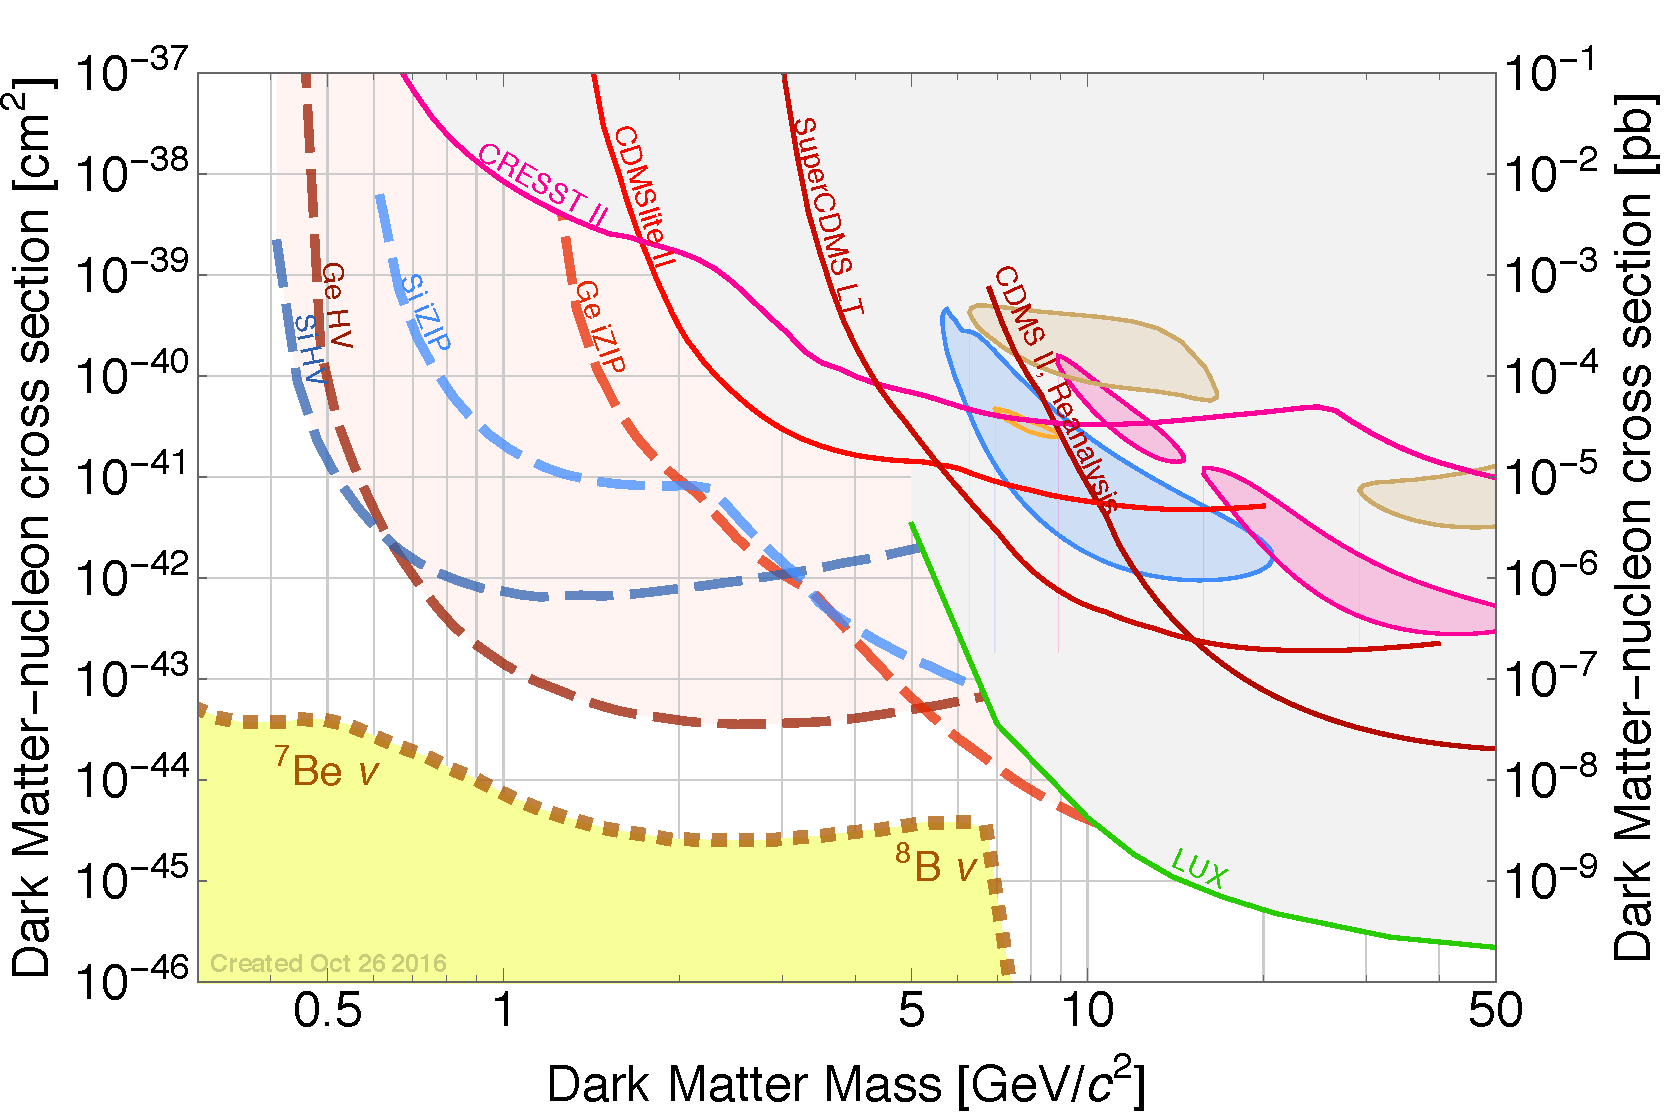
\includegraphics[width=\hsize]{Figures/SuperCDMS_Projected_Limits_squat.pdf}
\caption{\footnotesize Projected exclusion sensitivity for the SuperCDMS SNOLAB direct detection dark matter experiment~\cite{SuperCDMSSensitvitiy:2016arXiv}. The vertical axis is the spin-independent dark matter-nucleon cross section under standard halo assumptions ~\cite{Lewin:1995rx}, and the horizontal axis is the dark matter mass, where dark matter is used to mean any low-mass particle dark matter candidate. The blue dashed curves represent the expected sensitivities for the Si HV and iZIP detectors and the red dashed curves the expected sensitivities of the Ge HV and iZIP detectors. These sensitivity limits are determined using the Optimum Interval method~\cite{Yellin:2002xd}, which does not incorporate any knowledge of the specific disposition and source of background events observed during the experimental operation. The solid lines are the current experimental exclusion limits in the low-mass region, from the CRESST-II ~\cite{2012EPJC...72.1971A}, SuperCDMS \cite{Agnese:2014aze,Agnese:2015nto} and LUX ~\cite{Akerib:2015rjg} experiments. The dotted orange line is the DM discovery limit from~\cite{Ruppin:2014bra}, which represents the cross-section at which the interaction rate from dark matter particles becomes comparable to the solar neutrino coherent elastic scattering rate.
}
\label{fig:SIdataProjections}
\end{figure}


Over the past two years, the SuperCDMS collaboration has lead the field in the search for low-mass matter ($<$ 10 GeV/c$^{2}$).  The most recent results from CDMSlite, a mode where the cryogenic germanium detectors are operated at a relatively high bias voltage to amplify the phonon signal reached an energy threshold for electron recoils as low as 56~eV.  Based on 70 kg-days of exposure, these results excluded new parameter space for the dark matter-nucleon spin-independent cross section for dark matter masses between 1.6 and 5.5 GeV/c$^{2}$.  In 2014 the collaboration released results from the first SuperCDMS analysis focused on searching for low mass dark matter using the iZIP detectors.  At the time of publication, this result lead the field.  These results are highlighted in Figure~\ref{fig:SIdataProjections}.

Several collaborations (using different target materials and techniques) have reported potential signals of low-mass dark matter. In particular, an annual modulation in the detection rate was observed by the DAMA/LIBRA collaboration using NaI(Tl)~\cite{Bernabei:03rnc,Bernabei:08epjc}. %as target and has been later confirmed by the extended experiment DAMA/LIBRA~\cite{Bernabei:03rnc,Bernabei:08epjc} reaching a statistical significance of 9.3\,$\sigma$. 
Also, CoGeNT~\cite{Aalseth:11prl2,Aalseth:11prl,Aalseth:13prd}  (using a germanium target) and CDMS II ~\cite{Agnese:13prl} (with data from the Si detectors) have excesses in their data that are compatible with light dark matter with a mass of the order of 10~GeV/c$^2$. 
These observations are challenged by the negative results obtained by other experimental collaborations. 
XENON10, XENON100, LUX ~\cite{Angle:11prl,Aprile:12prl,Akerib:14prl} (based on Xe), the above mentioned germanium-based
CDMS II, EDELWEISS~\cite{Ahmed:2011gh}, and SuperCDMS Soudan~\cite{Agnese:13prl2,Agnese:2014aze}, as well as KIMS (with CsI), CRESST~\cite{Angloher:2014myn} (with CaWO$_4$),
PICASSO~\cite{Archambault:2012pm} (with C$_4$F$_{10}$), PICO 2L~\cite{Amole:2015lsj} (with C$_3$F$_{8}$), SIMPLE~\cite{Felizardo:2011uw}
(with C$_2$ClF$_5$) and COUPP~\cite{Behnke:2012ys} (with CF$_3$I) have obtained 
negative results, setting more stringent upper bounds on the 
dark matter-nucleon cross section. Figure~\ref{fig:SIdataProjections} illustrates the experimental landscape for the dark matter-nucleus spin-independent scattering cross section as a function of the dark matter mass.

%\section{SuperCDMS SNOLAB}
%The SuperCDMS SNOLAB experiment will be a next-generation (G2) direct dark matter search to explore the light mass (1-10~GeV/c$^2$) DM region, and ultimately reach the solar neutrino floor. The SuperCDMS SNOLAB project is being designed to provide a large, shielded, ultra-low-background cryostat capable of housing up to 186 solid state cryogenic detectors (31 towers) operating at temperatures in the 15-40 mK range. The initial SuperCDMS SNOLAB project baseline will have a 29\,kg payload, consisting of 2 towers of 4 Ge (11.1\,kg) and 2 Si (2.4\,kg) detectors operated in the ultra low energy threshold high-voltage CDMSlite mode (CDMS-HV), providing the best sensitivity for DM masses below $\sim$5~GeV/c$^2$, and an additional 2 towers of germanium and silicon iZIP detectors, which provide better sensitivity in the 5-10~GeV/c$^2$ mass range. Assuming 5 years of operation with 80\% livetime, we would obtain raw exposures of 44 kg-yr (Ge HV), 10 kg-yr (Si HV), 56 kg-yr (Ge iZIP), and 5 kg-yr (Si iZIP), respectively. The projected sensitivities of the different operation modes for this initial payload are shown by means of red and blue dashed lines in Figure~\ref{fig:SIdataProjections}.

%With these ultra-low backgrounds and ultra-low threshold detectors, this G2 experiment will have unparalleled sensitivity for low-mass dark matter, with two complementary targets (germanium and silicon). The goals is to achieve sensitivities $\sim$100 times better than the current limits at 10\,\gev, increasing to $\sim 10^{5}$ times better sensitivity at $\sim$1\,\gev. 

%The large cryostat and passive shielding provide the capability to expand the detector mass to the necessary level that would allow full exploration of the low-mass DM parameter space down to DM-nucleon cross sections where solar neutrino-nucleus scattering becomes significant (sometimes called the "neutrino floor"). This could be accomplished with a combination of SuperCDMS detector upgrades.

%\begin{figure}[ht]
%\begin{center}
%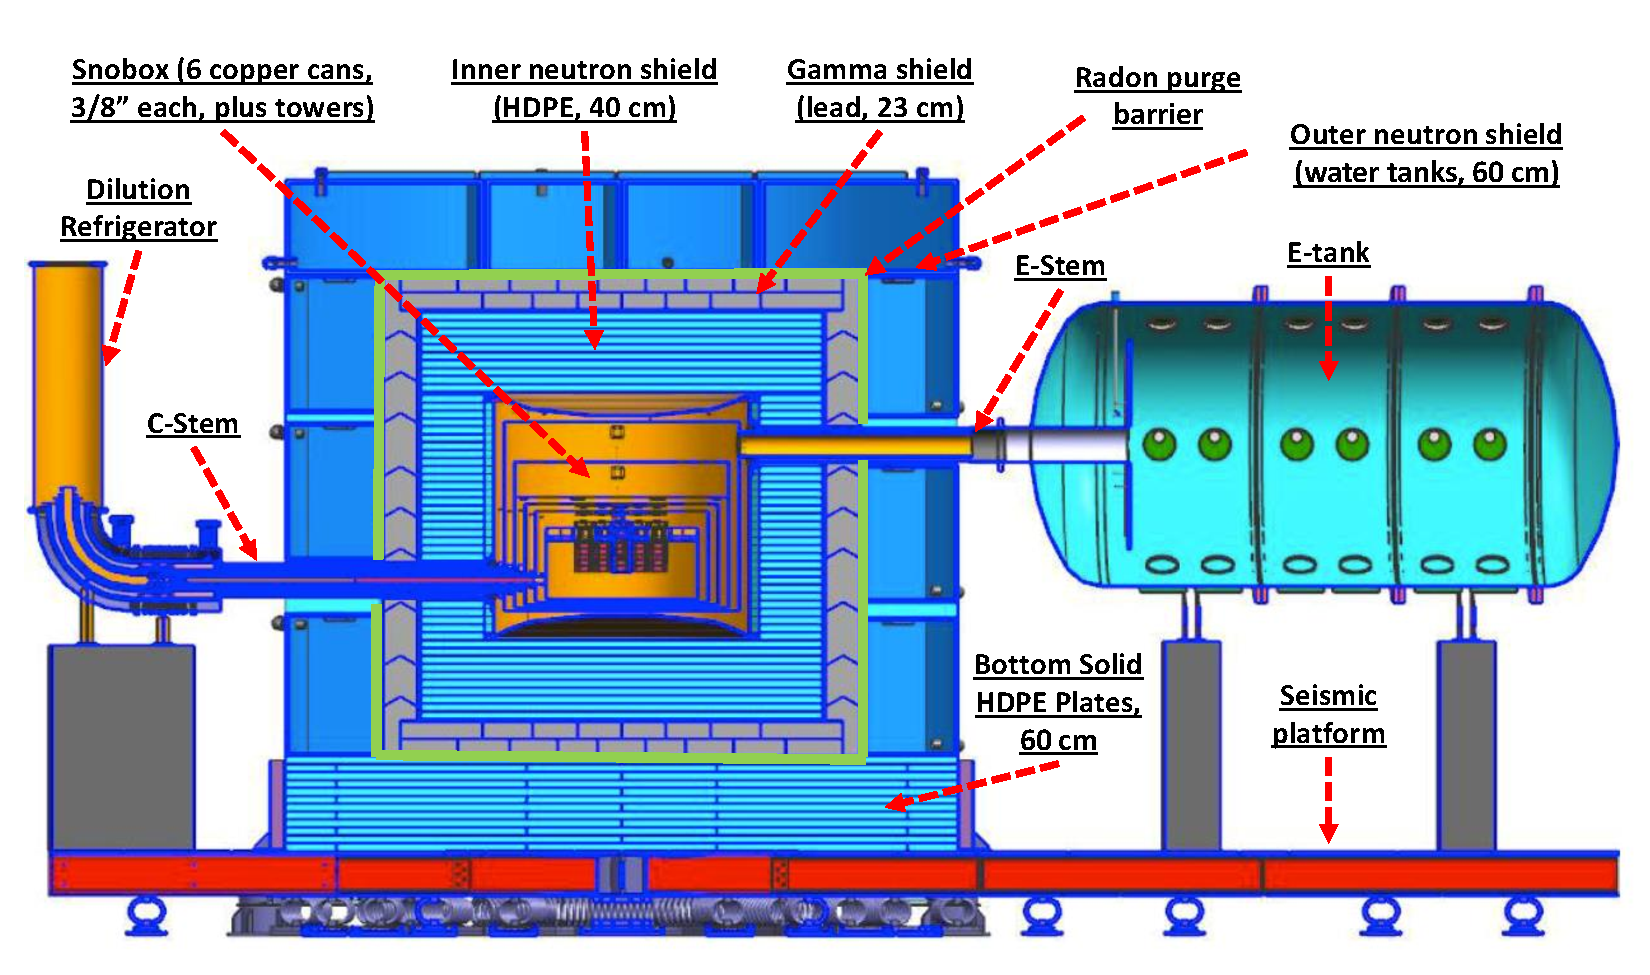
\includegraphics[width=0.8\textwidth]{Figures/f02_SuperCDMS_Schematic.pdf}
%\end{center}
%\caption{\footnotesize Sectional overview of the SuperCDMS SNOLAB conceptual design, showing some of the main features of the cryogenics and shielding systems.}
%\label{fig:overview}
%\end{figure}

%\subsection{\scs Science Goals}
%\label{subsec:science_goals}
%
%In Table~\ref{tab:sciencegoals}, we summarize the science goals for the experiment. We divide our science goals into three categories: primary, secondary, and future capability. The primary science goals drive the technical requirements, while the secondary science goals are examples of the rich set of science the data from this project will provide. The future capability science goal increases the science return from the investment made in the \scs project.
%
%\begin{table}[htbp]
%\centering
%\begin{tabular}{c}
%\hline
%Primary Science Goals \\\hline \\
%\parbox{\textwidth}{\textbf{SG-1} Search for dark matter with mass above 0.5 GeV in a Ge target without background discrimination (see Ge HV curve in Fig.~\ref{fig:SIdataProjections})\vspace{6pt}}\\
%\parbox{\textwidth}{\textbf{SG-2} Search for dark matter with mass above 0.3 GeV in a Si target without background discrimination (see Si HV curve in Fig.~\ref{fig:SIdataProjections})\vspace{6pt}}\\
%\parbox{\textwidth}{\textbf{SG-3} Search for dark matter with mass above 5~GeV in a Ge target with background discrimination (see Ge iZIP curve in Fig.~\ref{fig:SIdataProjections})\vspace{6pt}}\\
%\parbox{\textwidth}{\textbf{SG-4} Search for dark matter with mass above 1~GeV in a Si target with background discrimination (see Si iZIP curve in Fig.~\ref{fig:SIdataProjections})}\\ \\
%\hline 
%Secondary Science Goals \\\hline \\
%\parbox{\textwidth}{\textbf{SG-5} Search for non-standard dark matter interactions within the Effective Field Theory (EFT) framework \vspace{6pt}}\\
%\parbox{\textwidth}{\textbf{SG-6} Observe coherent neutrino scattering of $^8$B solar neutrinos\vspace{6pt}}\\
%\parbox{\textwidth}{\textbf{SG-7} Search for axions produced in the sun and relic axions\vspace{6pt}}\\
%\parbox{\textwidth}{\textbf{SG-8} Search for lightly ionizing particles (LIPS)\vspace{6pt}} \\
%\parbox{\textwidth}{\textbf{SG-9} Search for annual modulation} \\ \\
%\hline
%Future Capability Science Goal \\\hline \\
%\parbox{\textwidth}{\textbf{SG-10} Incorporate a pathway for future upgrades that would further increase the sensitivity of the experiment down to the neutrino floor in this low mass range, including deployment of advanced SuperCDMS detectors or those from the CRESST, EDELWEISS, and EURECA collaborations\vspace{6pt}} \\
%\hline
%\end{tabular}
%\caption{\label{tab:sciencegoals}Science Goals for SuperCDMS SNOLAB}
%\end{table}
%\clearpage

% !TEX root = NSF_SuperCDMS_SNOLAB_OPS.tex
\section{SuperCDMS SNOLAB (2 pages)}
\label{sec:snolab}

\begin{figure}
\centering
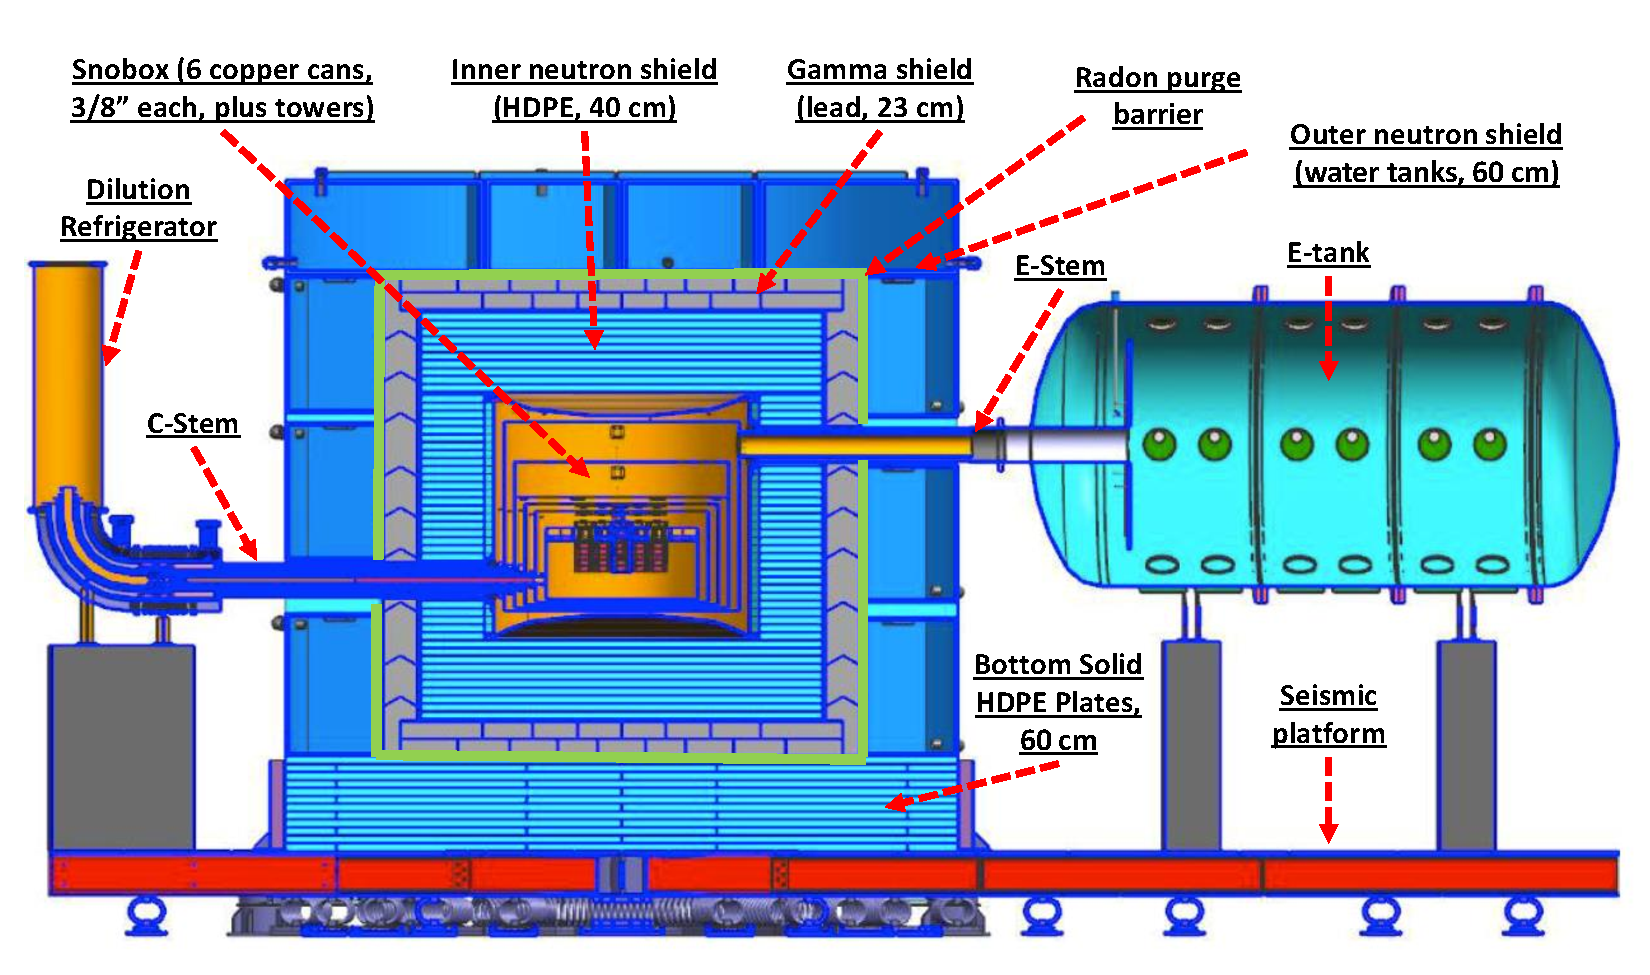
\includegraphics[width=0.8\textwidth]{Figures/f02_SuperCDMS_Schematic.pdf}
\caption{\footnotesize Schematic of the SuperCDMS SNOLAB experiment. The detectors reside within the inner can of the copper cryostat, and are shielded from the environment. A gamma shield protects from external gamma-rays and the inner polyethylene layers serve to absorb radiogenic neutrons emitted from the cryostat and gamma shield. The outer water tanks provide protection from external neutrons. The assembly rests on top of a seismic platform to provide isolation from seismic events. }
\label{fig:SCDMS_schematic}
\end{figure}

\begin{table}
\centering
\small
\begin{tabular}{  l  c  c  c  c } \hline
&\multicolumn{2}{c}{iZIP} & \multicolumn{2}{c}{HV}\\ 
&  Ge & Si    & Ge & Si \\ \hline
Number of detectors & 10 & 2 & 8 & 4\\
Total exposure (kg\(\cdot\)yr) & 56  & 4.8 & 44 & 9.6 \\
Phonon resolution (eV) & 50 & 25 & 10 & 5\\
Ionization resolution (eV) & 100 & 110 & -- & -- \\
Voltage Bias (V) & 6 & 8 & 100 & 100\\ \hline
\end{tabular}
\caption{The anticipated exposures and detector parameters for the SuperCDMS SNOLAB experiment. The exposures are based on 5 years of operation (from 2020--2024) with an 80\% live time. The quoted phonon energy resolutions represent the r.m.s.\ values of the total measured quantity (\textit{i.e.}, combining all active sensors). The quoted ionization resolution is derived from the readout electronics equivalent noise charge value of 33\textit{e} and represents the r.m.s.\ energy resolution of a single channel for electron recoils.}
\label{tab:ExpOperations}
\vspace{-20pt}
\end{table}


The SuperCDMS SNOLAB experiment will be a next-generation direct dark matter search specifically designed to explore the low mass ($<$ 10 GeV/c$^{2}$) dark matter region, with ultimate sensitivity to dark matter-nucleon cross sections where solar neutrino-nucleus scattering becomes significant (the so-called “neutrino floor”). The SuperCDMS SNOLAB G2 Project is being designed to provide a shielded, ultra-low-background cryostat capable of housing up to 31 towers of solid state cryogenic detectors.% operating at temperatures in the 15--40 mK range. 
The SuperCDMS SNOLAB Project baseline is outlined in Table~\ref{tab:ExpOperations}. The experiment will include a mixture of detectors composed of cylindrical germanium (Ge) and silicon (Si) crystals, 100 mm in diameter and 33.3 mm thick. Each Ge(Si) crystal will have a mass of 1.39(0.61)~kg. The detectors will be stacked into four towers of six detectors. Two towers of detectors will be operated in the ultra-low-energy threshold high-voltage mode (HV), providing the best sensitivity for dark matter masses below 5 GeV/c$^{2}$~\cite{Agnese:2015nto}. An additional two towers of germanium and silicon detectors will be operated in standard (iZIP) mode. These detectors will provide better sensitivity in the 5--10 GeV/c$^{2}$ mass range due to their capability to discriminate between electron-recoil and nuclear-recoil interactions ~\cite{Agnese:2014aze}. The anticipated exposure and detector parameters for SuperCDMS SNOLAB can be found in Table~\ref{tab:ExpOperations}. 

The detector towers will be cooled to ~15--30 mK using a dilution refrigerator and cryocoolers. The cold region of the full experiment, referred to as the SNOBOX, consists of 6 cylindrical copper cans suspended by Kevlar ropes. In the design, the SNOBOX is surrounded by a 40 cm thick layer of polyethylene to moderate and absorb neutrons produced by radiogenic contamination, and to provide a shield from external neutrons. This inner polyethylene layer is surrounded by a 23 cm thick gamma shield made from low-activity lead. The lead shield layer is surrounded by a thin metal shield to block radon (Rn) diffusion into the inner shielding layers. This volume will be purged with boil-off nitrogen gas to reduce the overall Rn levels and the backgrounds caused by prompt Rn daughters. The outermost shield layer consists of polyethylene and water tanks that provide additional shielding from the cavern neutron flux. A schematic of the experiment shield and cryostat layers can be seen in Fig \ref{fig:SCDMS_schematic}. 

The large cryostat and passive shield provide the capability to expand the detector mass to the necessary level that would allow full exploration of the low-mass dark matter parameter space down to dark matter-nucleon cross sections where solar neutrino-nucleus scattering becomes significant. This could be accomplished through a combination of SuperCDMS detector tower upgrades and incorporation of similar detectors from the EURECA collaboration.






%\clearpage

%Big Section: Plan of Work:
\section{Plan of Work (10 pages)}

% !TEX root = NSF_SuperCDMS_SNOLAB_OPS.tex
%% people who build community and knowledge
%% around software?
%% The maintainers
%% Educopia
%% http://ivory.idyll.org/blog/2019-communities-of-effort.html#disqus_thread
%% https://blog.dnanexus.com/2018-01-29-analysis-commons-a-collaborative-approach-to-multi-omics-discovery/

%% describing data
%https://library.si.edu/research/describing-your-data-data-dictionaries
%https://figshare.com/articles/The_State_of_Open_Data_Report_2017/5481187/1
%https://www.usgs.gov/products/data-and-tools/data-management/data-standards
%https://www.fgdc.gov/standards/standards_publications/
%http://www.ddialliance.org/ metadata standards for social sciences
%https://www.rd-alliance.org/groups/data-type-registries-wg.html research data alliance, not focused on physics AFAIK but definitely useful
%https://access-data.trydiscourse.com/
% XDR, external data format!!
% https://tools.ietf.org/html/rfc1832.html#section-6
% and there is a python library for it, xdrlib

% Mom says all the cool kids are using smartsheets
% Liquid Planner has a free plan for teachers?  https://app.liquidplanner.com/space/202855/projects

% documentation is often overlooked but people need it the most
% https://opensourcesurvey.org/2017/

\section{Solicitation-specific review criteria}
\subsection{Science-driven}
% How will the project outcomes fill well-recognized science and engineering needs of the research community, and advance research capability within a significant area or areas of science and engineering? What are the broader impacts of the project, such as benefits to science and engineering communities beyond initial targets, underrepresented communities, and education and workforce development? The project outcomes should address well-recognized science outcomes.

This project serves the immediate needs of researchers in the dark matter community and the experimental nuclear physics community by providing a common toolset for analyzing data in any format.

The PI expects that

\begin{itemize}
    \item Multiple research projects across the NSF directorate will be more productive because they can use existing, documented tools rather than building their own.  The PI intends to estimate this impact with citations from scientific papers.
    \item Increased involvement of undergraduate researchers in science analysis due to improved documentation and an extended support network.  The PI intends to measure this through undergraduate involvement in her own lab, community surveys, and tracking community forum data.
    \item Several example analyses will be publicly released, with accompanying documentation and support information for pre-requisite computing skills.  The intent is for these educational materials to be accessible to someone with no domain knowledge.  The PI believes these training materials will be an equitable training resource.
\end{itemize}


\subsection{Innovation}
% What innovative and transformational capabilities will the project bring to its target communities, and how will the project integrate innovation and discovery into the project activities, such as through empirical research embedded as an integral component of the project activities? Such research might encompass reproducibility, provenance, effectiveness, usability, and adoption of the components, adaptability to new technologies and to changing requirements, and the development of lifecycle processes used in the project.

A common limitation of data-analysis software that is entirely home-grown is that it does not scale as data grows and changes - a human has to update or rewrite the code if the requirements change substantially.

This library makes heavy use of existing libraries.  The benefit is that as those libraries improve and scale to larger data sets, this software inherits that improvement.  

In both cases, significant human effort is needed to adapt the software to changing data and needs.  But by leveraging well-supported, open-source libraries, the burden is shifted away from an individual scientist and towards an active community that is highly motivated to solve similar problems.  This library serves as sugar to allow scientists with many different data formats to take advantage of these popular libraries.

The danger to this approach is the same - if these libraries lose community support or focus on very different problems then this library will lose relevance over time.  To mitigate this risk, the PI is focusing on integrating with a library supported by the IRIS-HEP collaboration and with pandas, which enjoys extreme popularity in the data science community.

\subsection{Close collaboration among stakeholders}
% How will the project activities engage CI experts, specialists, and scientists and engineers working in concert with the relevant domain scientists and engineers who are users of CI?

The PI proposes to engage both cyberinfrastructure experts and the experimental nuclear physics community by (1) working closely with pilot experiments to build software that works effectively for scientists analyzing event-based data, (2) holding yearly workshops intended to foster interaction between the scientists using the software and cyberinfrastructure developers, and (3) attending conferences that will allow outreach to the scientific community (for example, the Low Energy Community Meeting) and the cyberinfrastructure community (for example, CHEP).

The PI has working relationships with scientists in the SuperCDMS collaboration and the XIA corporation, both of which are interested in exploring the proposed software as solutions to analysis needs.

In addition, the IRIS-HEP collaboration is interested in this work as it would extend their awkward-array library to a broader audience.  Awkward array was developed as part of DIANA/HEP \cite{diana-hep} and that effort will continue with IRIS-HEP \cite{iris-hep}
.  Collaborating with IRIS-HEP gives us access to experienced cyberinfrastructure developers who have focused on developing software suitable for terabyte-scale data.


\subsection{Building on existing, recognized capabilities}
% How will the project activities build on and leverage existing NSF and national cyberinfrastructure investments, as appropriate?

The proposed work builds on existing capabilities and communities in several ways:

\begin{itemize}
    \item \textbf{The PI proposes to use already-existing data description languages.}  The languages Katai Struct and the Data Format Description Langauage both have active communities and tools that work with data when provided a description.  Kaitai Struct is the target for the proposed work because (1) it is more human-readable than than the XML-based DFDL, and (2) Katai Struct generates code libraries that allow users to load their data into the programming environment of their choice; DFDL currently works by providing an XML or JSON equivalent of the binary data.  While this is a powerful approach because any language with an XML or JSON parser can now read the data, it also produces a secondary data file that is an order of magnitude larger than most binary files.  This makes DFDL, in its current state, unusable for scientists with gigabyte-scale data sets as it would make the required storage space for analysis prohibitively expensive.
    \item \textbf{The PI proposes to use already-existing infrastructure for the data-analysis library.}  Scientists who would like to avoid writing custom software to read their binary data can already use the Kaitai Struct compiler to generate libraries to read their data in python, C++, and a multitude of other languages.  The advantage is that there is substantial support documentation and an active community available for troubleshooting.  The disadvantage is that the current Kaitai Struct python compiler stores the data in a structure that does not provide adequate speed performance for gigabyte-scale data sets.  By improving the existing Katai Struct compiler software, we can build a science-ready analysis library and scientists can benefit from the existing community support and documentation.   
    \item \textbf{Use a supported and optimized data structure}  for the improvements to the Kaitai Struct compiler.  The ``awkward-array'' library was developed by DIANA/HEP and is now supported by IRIS-HEP and is part of a set of libraries designed to provide flexible data-analysis tools for the high-energy physics community.  The awkward-array data structure is optimized for fast queries on an event-based data set and as such is ideal for the majority of nuclear physics data.  By choosing this data structure as the target, we bring the optimized and convenient analysis environment of awkward-array to any scientist who describes their data with the Katai Struct language.
    \item \textbf{Provide analysis tools for the python environment and training materials that take advantage of the python ecosystem.}  Python is a popular analysis environment in the field of big-data and has enjoyed significant adoption in the scientific community; enough so that python support is compiled in the dominant high-energy physics software, ROOT, by default.  By providing a python library for data analysis, scientists can make use of a full ecosystem that supports data analysis: numpy for convenient array manipulation; scipy for fitting; matplotlib for producing publication-quality figures; and even numba for easy compilation of code that needs to run fast.  This entire environment is easily installed - even for users without administration privileges - through the Anaconda Python distribution.  There are many free and paid programming environments that are availble, notably the Jupyter environment.  Code written in this environment is particularly nice as a tutorial because it is rendered nicely on github, gitlab, and interactive notebooks can be opened in one click through binder.  By providing a small set of introductory documentation, scientists can benefit from the effort the python community has put in to lower the barrier for use.
    
\end{itemize}

\subsection{Project plans, and system and process architecture}
% For an "Elements" proposal, the Project Description should include a high-quality management plan. The proposal should include user interactions and a community-driven approach, and provide a timeline including a proof-of-concept demonstration of the key components. Software or data cyberinfrastructure services should be sufficiently described and follow industry best practices, including the architecture of the CI and the engineering process to be used for the design, development, documentation, testing, validation, and release of the software, its deployment and associated outreach to the end user community, and an acceptance and evaluation plan that involves end users. The description of the CI architecture and processes should explain how security, trustworthiness, provenance, reproducibility, and usability will be addressed by the project and integrated into the proposed system and the engineering process, and how adaptability to new technologies and changing requirements will be addressed by the project and built into the proposed system, as appropriate.


\textbf{Architecture of the software:}
The architecture of the Kaitai Struct compiler that targets an awkward-array data structure will follow that of the existing Katai Struct software.  Implementing a Kaitai Struct compiler for a new language requires

\begin{enumerate}
    \item Writing a ``runtime library'' that provides a standard stream interface in the target language.  For example, one of the functions every language needs to have defined is a method that returns the size of the file or string stream.  By writing a ``size'' function for the language of interest that follows the Katai Struct API, the code generation becomes simpler.
    \item Writing a ``compiler'' that translates Kaitai Struct concepts, implemented in Scala, into the target language.
    \item Writing a test runner for the new language. 
\end{enumerate}

The proposed work targets the python environment, and there is already a Kaitai Struct python compiler.  The ``compiler'' for the python implementation, however, stores data in native-python data structures that provide inconveniently slow access to standard queries on large, gigabyte-scale data sets.  

However, the changes that need to be implemented to instead store the data in the faster awkward-array data structure are restricted to the compiler code.  The runtime library provides a convenient interface for reading data from a file or stream - this code only cares about the file system interface and does not need to change.  The python test interface will need to be updated as the access syntax for the data will change slightly.

Although there is opportunity for improving the speed of the data load, this development will instead focus on adhering to the existing format and style of Kaitai Struct.  The goal is to make the existing Kaitai Struct community useful to scientists who work with gigabyte-scale data sets; waiting for a few minutes for the data to load is not ideal but is typical of many locally-built solutions.  We can address the more-critical issue of rapid data queries while staying well within the existing framework of Kaitai Struct and intend to do so for the initial implementation of the software.

If we find that data-load times are a significant issue for the nuclear physics community then we will consider more substantial changes to the Kaitai Struct compiler and runtime libary.

\begin{comment}
\begin{lstlisting}
def [*size(self)*]:
    # Python has no internal File object API function to get
    # current file / StringIO size, thus we use the following
    # trick.
    io = self._io
    # Remember our current position
    [*cur_pos = *]io.tell()
    # Seek to the end of the File object
    io.seek(0, SEEK_END)
    # Remember position, which is equal to the full length
    [*full_size = *]io.tell()
    # Seek back to the current position
    [*io.seek(cur_pos)*]
[*return full_size*]
\end{lstlisting}

\begin{lstlisting}
uint64_t kaitai::kstream::[*size()*] {
    std::iostream::pos_type [*cur_pos = *]m_io->tellg();
    m_io->seekg(0, std::ios::end);
    std::iostream::pos_type [*len = *]m_io->tellg();
    [*m_io->seekg(cur_pos)*];
    [*return len*];
}
\caption{The details of this code are not important.  What is significant is the name of this function, size(), and its behavior: find and report the size of the file, without changing where we are in the file.  The Katai Struct compiler for both C++ and python can use the ``size()'' function rather than including these language-specific stream commands, making the compiler code more readable.}
\end{lstlisting}
\end{comment}

\textbf{Architecture of the user documentation:} User documentation should make it possible for users with little to no domain knowledge to use the data-access library for science.  Documentation for the use of the library will be stored as text files in the repository with the code.  The files will be written in markdown syntax to improve their readability; this will also render them nicely on cloud-based repository hosts such as github and gitlab.  The following documentation will be provided:

\begin{enumerate}
    \item How to get help with questions or issues about the library.
    \item How to install the library and its dependencies.
    \item An overview explaining what the user will need to provide (data and a description of the data) and what the library will provide (software to read that data).
    \item A tutorial walking through the use-case of a scientist looking at simple data with a custom format.
    \item Links to additional resources detailing more complex data formats and more complex analyses.
    \item Citation guidelines.  
\end{enumerate}


\textbf{Architecture of the developer documentation.}  Documentation intended to facilitate development of the code will be stored in the repository alongside the code.  Text files referenced in the top-level README file will detail, for every repository,

\begin{enumerate}
    \item How to install, develop, and test the code for individuals who wish to make changes.  
    \item How to contribute changes back to the project.  This will provide instructions on the version control practices used by the repository maintainers and instructions for implementing the tests required for changes to be considered for merging with the main code base.
\end{enumerate}

\textbf{Architecture of the basic scientific computing skills documentation:}  Documentation of basic computational skills and concepts will have several possible forms: (1) Text and images, (2) tutorial videos, (3) jupyter notebooks, (4) printable images that illustrate a focused concept, and (5) links to recommended resources such as Software Carpentry tutorials.

All materials will be licensed with  a permissive, open-source license such as CC-BY or MIT.  The source for all the materials will be publicly available through a public host such as github or gitlab and will be archived on a content-tracker such as the Open Science Framework or Figshare.  Videos will be released on YouTube and licensed CC-BY.

All materials will be disseminated using a static site generated by Antora.  Antora is specifically designed for documentation and allows a user to specify a set of repositories containing text files formatted in the Asciidoc markdown language to build a single, searchable documentation site.  Because Antora generates a static site, free hosting services are readily available.  This solution allows my students to focus on creating material to explain core concepts and practice interacting with version control rather than spending time wrestling with web development.

The topics students choose to document are largely student-led, with some guidance from the PI.  Spring 2019 marks the inception of this project, and the concepts chosen by students for illustration have focused on (1) tutorial-format guide for installing python and running a basic python-based analysis of gamma spectroscopy data, (2) instructions for using a docker container to simplify installation of a complex software environment, and (3) a poster explaining what an executable file is.

Documentation that will be provided in this format alongside the scientific computing resources will include

\begin{enumerate}
    \item instructions on where to get help with the material and how to provide feedback and and file bug reports
    \item instructions for those who wish to contribute to the documentation
    \item instructions for the deployment of the documentation
\end{enumerate}


\textbf{Engineering processes:}
% design, development, documentation, testing, validation, and release of the software
% and
% description of the CI architecture and processes should explain how security, trustworthiness, provenance, reproducibility, and usability will be addressed by the project and integrated into the proposed system and the engineering process
A primary goal of the proposed work is to build software that can be supported and maintained by the community.  A primary risk of the proposed work is staff turnover and associated loss of knowledge and onboarding time.

The software design, development, documentation, and testing work together to make it easy for the community to contribute to the software development - a goal that mitigates turnover risk as well.

The design process of the software will start with project documentation that describes (1) use cases, (2) requirements, (3) assumptions, (4) key decisions, and (5) definitions.  Such documentation is particularly useful for programmers who lack experience in experimental nuclear physics data analysis and makes it easier for skilled experts to contribute to the project.  This documentation also serves as a way to focus community discussions into defining a minimum useful scope for the software.

The development of all software in the PI's lab is done using version control software (git) and a central ``repository server'' that everyone interacts with.  Cloud-based servers such as github and gitlab are used because they are easy to use, provide robust backups, and also serve as a platform for dissemination and collaboration.

The PI's approach to version control and software releases prioritizes (1) easy-to-get, working code and (2) rapid updates.  This is implemented by building end-to-end tests and configuring automatic test running triggered by any changes to the repository.  Rather than insisting on a specific release cycle, developers are encouraged to put their changes on the public, master branch if their code is non-breaking.  Code on the public, master branch MUST pass all tests.  Semantic versioning will be used to alert users to breaking changes.

Work that breaks tests MUST be maintained on a separate ``branch'' that is publicly available but that will only be available to users by explicit action.  Instructions for developing code on such a branch will be included in the contributions documentation.

The key to this type of development is building simple end-to-end tests, implementing an automated testing framework, and investing heavily in documentation and testing of that documentation up front.  This development strategy works well for the proposed project because the software goal is already well-defined and the initial plan for implementation - leverage the existing Kaitai Struct framework as much as possible - is clear.  In addition, this development strategy is well-supported by community solutions and the organization of the PI's lab:

\begin{itemize}
    \item end-to-end testing of python code - and even tutorial notebooks in jupyterlab format - enjoy a thriving ecosystem in Python.
    \item many automated testing frameworks are designed specifically to support developers using cloud-based repository hosts such as github and gitlab; many are freely available to open-source projects.
    \item novices are always on hand to test documentation.  The PI maintains a group of approximately six students, many of whom have minimal experience with scientific computing.  Giving them goals such as: work through this example analysis and obtain a similar plot exposes conceptual gaps and problems with the documentation while providing excellent training for the student.  In addition, students have responded well to the opportunity to make a substantive contribution to the lab.
\end{itemize}

In summary, the proposed code development will be strongly tied to documentation, automated testing, and documentation testing.

%\subsubsection{Security}

\subsubsection*{Trustworthiness}
End-to-end tests of the software will include tests where the outcome is known.

\subsubsection*{Provenance}
All releases will be archived with their own DOIs on Zenodo.  Guidance to cite the version of the software used will be included in the top-level README of all releases and posted on all related websites.

\subsubsection*{Reproducibility}
End-to-end tests of the software will completely define all inputs, including a reference data set, and compare the output to reference products such as histograms.  The PI acknowledges that this is in no way a complete test of reproducibility but feels that it will be a useful starting point.  

Instructions for system setup will be included in the documentation.  Full or partial system specifications are required for automatic test running and will be versioned together with the rest of the code.  The most popular of these, Docker, will be used.  More complete system specifications as provided by Nix and Guix will be considered if need arises for more complete reproducibility.

\subsubsection*{Usability}
For the proposed software, usability consists of several scenarios:

\begin{tabularx}{\textwidth}{XX}
    Can a scientist easily use this code to do data analysis on a custom-format data set? & \\
    \toprule

    Is the scientist aware that this software exists?  Can the scientist find the software easily even if all they recall is a vague description?
    & Publications citing DOIs hosted on Zenodo with published preprints; well-indexed project website; open development on github, gitlab; indexed on python library repositories where appropriate \\
    Can the scientist install the software on their analysis computer easily, with or without root access?
    & Installation documentation; testing of installation documentation by novices; review of systems that need installation support at workshops \\
    Does the software apply itself well to this particular analysis need?  Can the scientist see how to use the software in their analysis?
    & Example analyses; testing of example analyses by novices; creation of a ``now you try'' document to test effectiveness. \\
    Does the scientist know where to get help or discuss issues with the software?
    & All documentation and code will contain a header directing users to the project forum and repository issue tracking. \\


Can an interested individual contribute to the development of the software easily? & \\
\toprule

    Is there a clear description of the requirements and purpose of the software so that developers can decide if they'd like to participate?
    & Requirements documentation and a description of use cases will precede all programming work and will be versioned with the rest of the code.\\
    Is it clear where to get help or discuss the code?
    & All documentation will link to the forum and the repository issue tracker.  The forum will be configured for web crawlers to maximize its discoverability.\\
    Are there clear and complete instructions on testing the software locally?
    & Local and remote testing infrastructure is as high in priority as the initial development of the code; documentation will be written as part of the first efforts.  Students will test these local development instructions.  Instructions may reference the scientific computing documentation.\\
    Are there clear and complete contribution instructions?
    & Contribution instructions will be developed with high priority once there is an initial passing test, even before there is functioning code.  Students will test these contribution instructions.  Instructions may reference the scientific computing documentation.\\
\end{tabularx}


\subsubsection*{Adaptability}
The proposed software intends to support scientific analysis of gigabyte-scale data for the coming decade.

The benefits of the proposed software, compared to the current, group-driven methods, are increased access to scientific analysis through ease of use, quality documentation, and community support.  And improved return on invested maintenance time, since effort on a common set of tools can benefit many scientists.

Another advantage of the proposed software is that it leverages existing, well-supported projects to deliver science-ready software.  Adaptations to changing data needs and opportunities can potentially come from efforts outside nuclear physics.

There is always the possibility that these dependencies could be abandoned.  Archives of all dependent software will be made as a safeguard against this.  Other risk mitigation the PI will pursue is significant investment in automated testing and documentation, particularly interface documentation.

\subsection{Deployment and user outreach:}
A key component of the user outreach will consist of annual workshops designed to promote hands-on use of the software and close collaboration with the software developers.  To maximize the effectiveness of these workshops,

\begin{itemize}
    \item Participants will be contacted in advance to begin early coordination of the analysis they're interested in doing with the data-access library
    \item Communication before and after the workshop will be encouraged through the maintenance of an open forum
    \item Prototype software will be released along with installation documentation, an example analysis, and contribution documentation prior to the workshop and tested by novices
    \item Discussion of the community roadmap will be integrated into the workshop and a new release of the roadmap will follow each workshop
    \item The conference will be registered on the Open Science Framework, providing an archived record of material prepared by participants.
\end{itemize}

Deployment of this software will use common open-source channels such as github, gitlab, and python package indexes such as PyPI and Conda.  Github and Gitlab both provide static page serving for projects.

Project communication will use the built-in issue tracking provided by repository hosts and open forum software such as Discourse.  Live-chat is not an anticipated need, but if it becomes clear this would be useful then the PI will consider using freely-available chat services such as Slack, Zulip, or Gitter.

Deployment of the software will also happen through academic channels such as preprint servers, project releases on the Open Science Framework, and/or Figshare.



\subsection{Acceptance and evaluation:}

Community adoption of this software is central to the success and broader impact of this project.

The simplest evaluation metrics of community adoption and use will be (1) citations of software in peer-reviewed scientific papers and (2) the number of contributions to the code from developers outside the PI's group.

Additional metrics that may provide useful information could include: (a) number of downloads from the Zenodo or gitlab site and (b) quantity of interactions on the issue tracker and forum.

The PI intends to use interviews to understand how the software meets (or not) the needs of the community.  The yearly workshops will provide an ideal setting for such discussions.  In addition, a standing feedback survey will be linked from the project page to capture responses from the people who have the time and willingness to share.

This feedback will directly inform decisions about priorities and have an official outlet in the release of an annual roadmap.  Discussion and contribution to the roadmap will be open to the community and will begin at the yearly workshop.


\subsection{Deliverables}
% Does the proposed project clearly articulate the services and capabilities to be delivered, and how they are to be delivered? NSF encourages exploration of various delivery mechanisms, including but not limited to, those leveraging eXtreme Science and Engineering Discovery Environment (XSEDE), leadership-class computing resources, OAC Software Institutes, Big Data Regional Innovation Hubs, individual organizational resources, and well-known public and private cloud services.

\subsection{Metrics}
% Does the proposed project clearly articulate quantifiable metrics for development and delivery of the services and capabilities to be delivered by the project, and for the anticipated community adoption and usage? Are quantitative metrics with targets identified for each year of the award? These should be simple but should also clearly show what the project will accomplish each year, the impact on science, and the breadth of the user community.
The simplest evaluation metrics of community adoption and use will be (1) citations of software in peer-reviewed scientific papers and (2) the number of contributions to the code from developers outside the PI's group.

Additional metrics that may provide useful information could include: (a) number of downloads from the Zenodo or gitlab site, (b) quantity of interactions on the issue tracker and forum, and (c) materials provided by data-sharing platforms that educate scientists on data-description languages.

Another informal metric of community support is how many scientists apply to the yearly workshop who are not actively solicited by the group and individual interviews with scientists using the software.

\subsubsection*{Year 1}
An initial release of the improved software and the XIA library is made.  Both have basic testing coverage, are tested automatically upon commit, and have initial guidelines for contribution.  An initial release of the skills documentation has been made.
\begin{itemize}
  \item A whitepaper is published describing data description languages and giving use-cases
  \item No citations of the software library are expected from peer-reviewed science results in year 1.
  %\item The Open Science Framework and Figshare are contacted.  We find out if they're interested and if so, get a contact person.
  \item Between 15 and 20 scientists register for the Data Access workshop.  These scientists are expected to predominantly come from the nuclear physics community.  The PI expects all attendees to register after specific invitation.
  \item Between 2 and 5 scientists register projects with the Open Science Framework or similar platform to work on analysis of their data collaboratively
  \item An initial release of the improved software and the XIA library is made.  Both have basic testing coverage, are tested automatically upon commit, and have initial guidelines for contribution.
  \item Inexperienced students who try to follow the analysis tutorial are able to find answers to some of their questions but most are expected to be unable to complete the tutorial without expert assistance
  \item Interviews with scientists attending the workshop show that out of ten scientists: approximately two find the software useful as-is for their analysis work; approximately five would find the software useful but do not plan to use it because of solvable issues; and approximately three do not plan to use the software either because it is not useful to them or because their issues with the software cannot be easily addressed.
\end{itemize}

\subsubsection*{Year 2}
The highest-priority improvements as identified by the community roadmap are released.  The contribution guidelines and instructions are well-tested.   The most common failings of the skills documentation have been addressed. 

\begin{itemize}
  \item At least one peer-reviewed science result cites the data-access library.
  \item Between 15 and 20 scientists register for the Data Access workshop.  Some diversity of discipline is expected, although most are expected to predominantly come from the nuclear physics community.  The PI expects one or two attendees to find out and register for the conference from someone outside the group and for most to register after specific invitation.
  \item Between 3 and 7 scientists register projects with the Open Science Framework or similar platform to work on analysis of their data collaboratively
  \item  There has been at least one request for an improvement or feature from the community that has been either fixed by my team or another contributor.
  \item  Inexperienced students who try to follow the analysis tutorial get stuck on these issues less frequently.  Most are able to complete the tutorial without expert assistance but are unable to make significant progress on the ``now you try'' analysis tutorial without expert assistance.
  \item Interviews with scientists attending the workshop show that out of ten scientists: approximately four find the software useful as-is for their analysis work; approximately four would find the software useful but do not plan to use it because of solvable issues; and approximately two do not plan to use the software either because it is not useful to them or because their issues with the software cannot be easily addressed.
\end{itemize}

\subsubsection*{Year 3}
The highest-priority improvements identified on the road map for the core library are released.  The contribution guidelines and instructions are well-tested.  The basic-skills documentation has resources or recommends resources that address most of the questions that arise when inexperienced students try to follow the analysis tutorial.  

\begin{itemize}
  \item At least five peer-reviewed science results cite the data-access library.
  \item Between 15 and 25 scientists register for the Data Access workshop.  Some diversity of discipline is expected, although most are expected to predominantly come from the nuclear physics community.  The PI expects at least three attendees to find out and register for the conference from someone outside the group and for most to register after specific invitation.
  \item Between 5 and 10 scientists register projects with the Open Science Framework or similar platform to work on analysis of their data collaboratively
  %\item The highest-priority helper code is close to stable.  The contribution guidelines and instructions are well-tested.  There has been at least one request for an improvement or feature from the community that has been either fixed by my team or another contributor.
  \item There has been at least five requests for an improvement or feature from the community that has been either fixed by my team or another contributor.
  \item Inexperienced students can independently find answers to most of their questions when following the analysis tutorial.  Most students still need expert help on the ``try your own'' analysis tutorial but find it easier to formulate their questions
  \item Interviews with scientists attending the workshop show that out of ten scientists: approximately six find the software useful as-is for their analysis work; approximately two find the software useful as-is but would very much like to see one or several non-trivial issues addressed; and approximately two do not plan to use the software either because it is not useful to them or because their issues with the software cannot be easily addressed.
\end{itemize}


\subsection{Sustained and sustainable impacts}
%The Project Description should address how the project outcomes and its activities will have long-term impacts, and how these will be sustained beyond the lifetime of the award, as appropriate. Manuals and tutorials for using the developed CI should be delivered to the community. Software or data cyberinfrastructure services must identify the intended license to be used for the released CI, and the justification for the choice of this license. PIs who have been previously funded under previous CI awards should show quantifiable evidence of the use, impact and sustainability of the previously funded work (and include a citation to the published CI in their biographical sketches as one of their relevant products, if appropriate).

The goal of the proposed work is to significantly increase the accessibility of scientific data analysis on custom-format binary data.

The proposed work will not eliminate the need for developing custom software within institutions and groups - but the project will provide a common toolset that will work for the majority of gigabyte-scale, event-based analysis despite the lack of a uniform data format.  The success of this project is expected to

\begin{itemize}
    \item Reduce redundant time spent on writing custom data-access software
    \item Reduce experts' time spent fighting with existing software during analysis
    \item Significantly increase the involvement of students in the science-analysis phase of research
    \item Improve the reproducibility of science results 
    \item Allow software development to occur in an environment where credit for this often-invisible work is possible
\end{itemize}

The success of this project depends on significant community involvement; the PI believes that the flexible nature of the proposed software, its immediate need for many in the community, and the community-building work of the grant can achieve this goal.

The plan for long-term sustainability of this project is twofold.  (1) The scope of the proposed software is small and the PI expects this software to be in a mature state by the end of these funds.  Therefore the project is expected to require less effort from the core development team.  (2) It is expected that the work proposed will build a broad community of users and developers who will continue to support the software because it is directly useful to their science goals.

In addition to hoping that the community developed during the course of this funding will be able to maintain the software at a usable level, the PI will investigate possible support from organizations like NumFOCUS as well as the Open Science Framework and Figshare. 
\clearpage

\section{Experiment Performance, Calibration, and Optimization}




\subsubsection{Detector Performance (1.5 pages)}

\clearpage




\subsubsection{Detector Calibration (1.5 pages)}

\clearpage



\subsubsection{Detector Optimization (1.5 pages)}

\clearpage



\subsubsection{Background Studies (1 page)}

\input{4f-POW-Commissioning}

% !TEX root = NSF_SuperCDMS_SNOLAB_OPS.tex
\section{Underground Test Facilities}
\label{sec:nexuscute}

A large part of this proposal is to perform critical measurements that require lower background environments than what has been available at our collaboration's surface test facilities. When operated at the surface, large cryogenic detectors can become swamped with cosmogenic background. Detailed detector performance properties, such as their discrimination power and behavior in the actual experimental environment, cannot be tested at surface facilities.

In this section we introduce two new underground sites that will be central to a large fraction of this work. The Cryogenic Underground TEst facility (\cute) is being built by the \SuperCDMS group at Queen's University and will be situated at \SNOLAB. The Northwestern EXperimental Underground Site (\nexus) is being built by the Northwestern University group and will be located in the MINOS near-detector hall at Fermilab. 

At the core of each facility is a cryogen-free dilution refrigerator equipped with special provisions to minimize the level of vibrations that may be introduced by the pulse tube cooler that provides the cooling down to 4~K. Both refrigerators provide a large cold volume that can house a SuperCDMS tower with a full complement of 6 detectors, and both are surrounded by a passive shield to lower radiogenic backgrounds. The two facilities are complementary. With a target background rate of $\sim$2~events\perkkd, \cute will offer lower overall backgrounds and radon mitigation, allowing for production \scs towers to be installed and tested. It is a low-background facility fully capable of cutting edge science. With a target background rate of $\sim$100 events\perkkd, \nexus is better described as a prototyping and R\&D facility, with less stringent background controls but more flexibility in its configuration and accessibility. Both still qualify as low-background environments when compared to surface facilities, which have a background rate of $\sim 10^4$\perkkd. This is why a number of calibration and detector characterization studies can be performed at \nexus and \cute that would be difficult or impossible to perform at a surface installation.\MP{There is no discussion of nuclear recoil backgrounds}.

\MP{Shouldn't we say that wiring / readout / grounding schemes / DAQ for these underground facilities is identical to that of SuperCDMS. A huge part of our argument is that work at these 2 facilities minimizes commissioning time of SuperCDMS SNOLAB}

\subsection{CUTE}
\label{sec:cute}

The \cute facility will be located in the Ladder Lab at \SNOLAB, next to the \SuperCDMS experiment. The cosmogenic background is therefore negligible, making the radiogenic backgrounds at \cute dominant. The dilution refrigerator will be placed inside a dry-well in the center of a water tank with a diameter of about 3.7 m and a height of about 3.2 m. The water acts as shielding material against external gamma and neutron radiation \MP{it's ultrapure water sourced from SNO right?}. The water layer thickness is about 1 m on the bottom and 1.5 m on the sides. The dry-well and the refrigerator itself generate an opening in the shielding on the top of the setup. Early Monte Carlo simulations for such a setup indicate an external gamma rate of order of 100 events\perkkd, strongly dominated by gammas entering directly from the top. In order to reduce the external gamma ray flux, and to protect the detectors from radiation that may originate from the dilution unit of the refrigerator, a 15 cm thick disk of lead is mounted inside the refrigerator, between the cooling unit and the detectors. The residual background for this setup was estimated to be a few tens of events\perkkd. The addition of an additional layer of lead inside the dry-well (15 cm at the bottom and 10 cm on the side walls, totaling $\sim$4 tons) is expected to reduce the external background by another order of magnitude. This background level of $\sim$2~events\perkkd\ allows for the measurement of the intrinsic \isotope[32]{Si} background in \scs detectors and opens the possibility of dark matter science prior to the start of \scs.

The \cute refrigerator has been ordered and is expected to be delivered to Queen's University for confirmation of performance in May 2017. The installation of the water tank and deck structure for access to the facility will begin in early 2017 so that the infrastructure is ready in summer 2017 when the refrigerator is expected to be delivered to \SNOLAB. The commissioning phase of \cute at \SNOLAB is expected to begin in late summer or early fall 2017.


\subsection{NEXUS}
\label{sec:nexus}

\begin{figure}
\centering
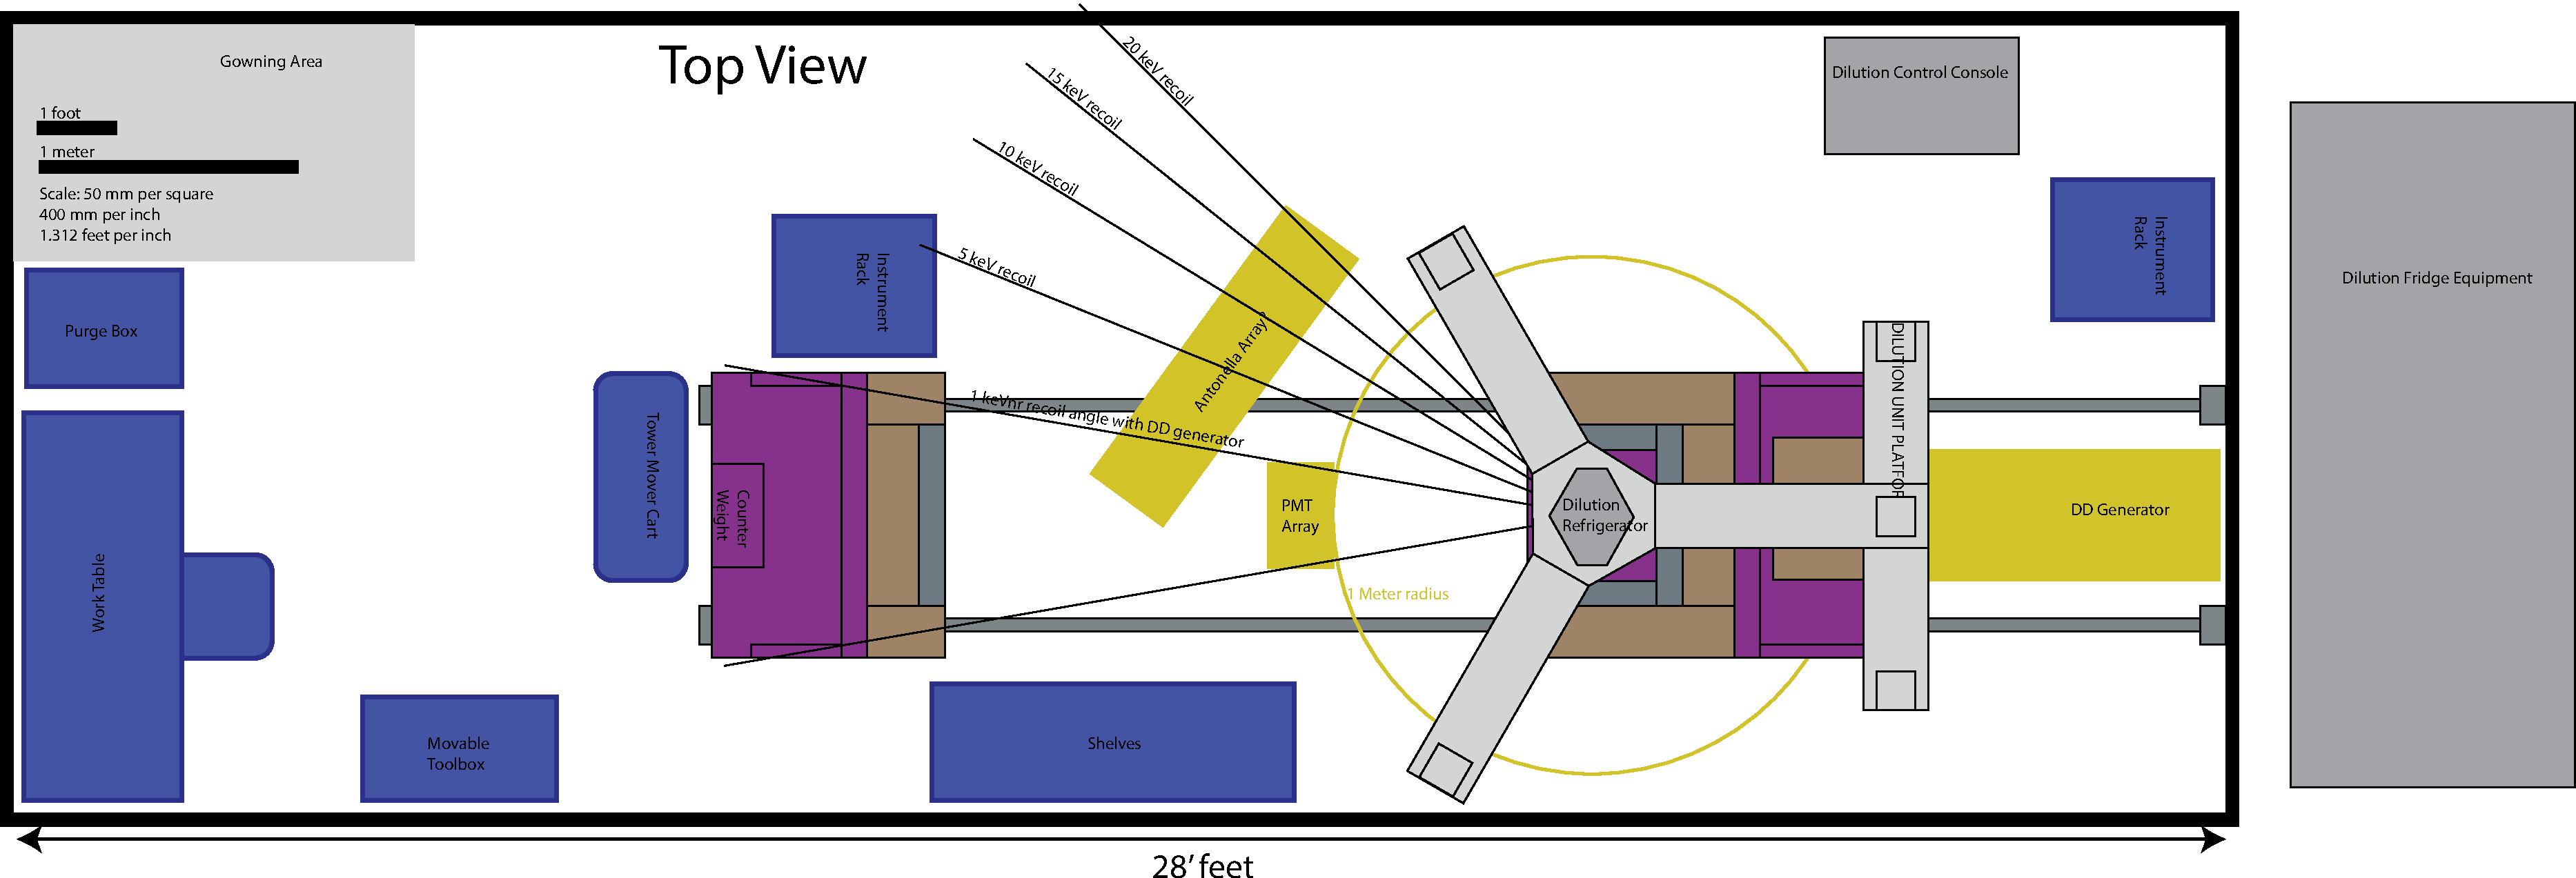
\includegraphics[width=\textwidth]{Figures/NEXUS-Layout-YieldMeas}
\caption{\nexus layout schematic. The outer box delineates the clean room to be placed 100 m underground in the \numi access tunnel. The blue boxes are support equipment, while the grey, brown, and purple structures are the passive shield, which is on rollers and half of it is moved out to the left to allow the neutron backing detectors to be placed. The D--D generator (described in Section~\ref{sec:ddcal}) is shown as a yellow box on the right, with neutrons passing through a collimating hole in the shield toward the detectors. Neutrons hit the HV detectors in the dilution refrigerator and scatter into angles as labeled depending on the recoil energy. An existing array from Fermilab will cover the wider angles between up to 20~keV, while a purpose-made fine-grain neutron detector PMT array will cover the recoil energies below 1~keV.\vspace{-2ex}}
\label{fig:nexus}
\end{figure}

\nexus is a testing facility planned for the MINOS near-detector hall at Fermilab ( 100~m underground). It will operate a dilution refrigerator surrounded by a 10~cm lead and 20~cm poly shield in a clean room environment. The rock overburden removes all muon-induced hadronic showers and lowers the muon flux to 0.5 muons/m$^2$/s. The lead shield (which includes a disk-shaped shield inside the refrigerator similar to \cute) will reduce the background to less than 100~events\perkkd. This facility is being built through a collaboration between Northwestern University and Fermilab.  A schematic of the calibration setup described in Section~\ref{sec:ddcal} is shown in Figure~\ref{fig:nexus}. The design of the clean room facility, the structural support for the dilution refrigerator, and the passive shield mechanical design are all underway. Installation of the dilution refrigerator is expected in fall of 2017, and the facility will be operational by the end of that year.


\subsection{Electronics and Shielding for \SuperCDMS Detectors}
%\comment{This probably belongs in the budget justification or somewhere else}

Much of the \scs hardware required to perform the measurements and science outlined in this proposal, such as pre-production towers and detectors, will be made available after the items are no longer needed for the \scs project. There are several exceptions, which are budgeted in this proposal and described here. To complete the measurements in this proposal at \nexus, the ability to read out two detectors is required. For \cute, a full contingent of 6 detector readout channels is needed for the science measurement. Thus we request: 

$\bullet$ Detector Control and Readout Cards (DCRCs). Two DCRC's are required to read out each HV detector, so we budget 4 for \nexus and 4 for \cute to test pre-production detectors. The HV tower will have its own DCRC's that will move to \scs with the tower.

$\bullet$ 300 K--4K wiring. The wiring to connect the DCRCs to the towers needs to be provided. Four are available for use at \cute, so we budget 8 more (we need 12 to read out the tower) and 4 for \nexus.

$\bullet$ Lead shield for \cute. The order of magnitude background reduction provided by this shield will provide sensitivity to the  \isotope[32]{Si} signal and the potential for early dark matter science. The shield for \nexus is already part of the facility.




%\clearpage

% !TEX root = NSF_SuperCDMS_SNOLAB_OPS.tex
\section{Pre-Operations and Commissioning Tasks}
\label{sec:operations}

The \SuperCDMS collaboration has had two decades of experience in operating underground dark matter experiments at Stanford and Soudan. The `lessons learned' from this experience are being applied as we develop our pre-operations, commissioning, and operations models for the \scs experiment. In this section, we discuss the main activities that will be conducted during this three-year proposal. These follow from the objectives listed in Section~\ref{sec:overview}, and are organized in a work breakdown structure as follows: 

\begin{table}[h]
\centering
\begin{tabular}{ll}
\multicolumn{2}{l}{\WBS Descriptions}\\\hline
1.1 & Calibration of Si and Ge \scs Detectors\\
1.2 & Performance Optimization of \scs Detectors \\
1.3 & Early \scs Science\\
1.4 & \scs Commissioning\\
1.5 & Education and Public Outreach\\
%\hline
\end{tabular}
\caption{Work Breakdown Structure for this proposal, based on the objectives laid out in Section~\ref{sec:overview}.}
\end{table}

The first two activities in the \WBS are measurements essential to the scientific output of the \scs experiment. The third activity provides the potential for early world-leading low-mass dark matter results, which will not only have the potential for discovery, but provide training and publications for our young scientists in the collaboration. This proposal's fourth activity is the commissioning of the \scs experiment, clearing the final hurdle for operations to begin. The final activity is the education and public outreach component of the Broader Impacts of this proposal.
The following sub-sections detail the work to be done in each of these activities.

  
%%%%%%%%%%%%%%%%%%%%%%%%%%%%%%%%
% Calibration is big so goes in its own file:
% !TEX root = NSF_SuperCDMS_SNOLAB_OPS.tex

\subsection{Calibration of Si and Ge \scs Detectors (\WBS 1.1)}
\MP{
\begin{itemize}
	\item rename to measure the nuclear recoil ionization yield at very low energies
    \item I think we should add a section on testing the electronic recoil calibration signal using LEDs
    \item we need to write this section with the understanding that 0V operation has a natural nuclear recoil ionization scale.
\end{itemize}
}

\label{sec:calibration}

A major focus of the SuperCDMS pre-operations program is to measure the nuclear recoil energy response in both Ge and Si down to 100 eV and eventually down to $\sim$30\eV.  This will match the energy thresholds we expect to achieve with the initial experiment and with upgraded detector towers.  These measurements are crucial for optimizing the operational parameters of, as well as achieving science in the next three years with the first production HV SuperTower at the Cryogenic Underground TEst (\cute) facility in \SNOLAB. Thus it is important to perform these measurements as early as possible, ideally completing them before data taking with the HV tower at \cute begins.

The signature of a WIMP-like dark matter interaction is a spectrum of low-energy nuclear recoils. \MP{WIMP DM is excluded < 10GeV ... we are looking largely for assymmetric dark matter models} The nuclear recoils produce both ionization and phonons.  The ionization yield (also know as quenching factor), which is the fraction of recoil energy that goes into the ionization, is recoil energy dependent.  A calibration of the nuclear recoil energy scale requires a measurement of the ionization yield, both its mean and its distribution, for all recoil energies of interest.

% The signature of a WIMP-like dark matter interaction is a spectrum of low-energy nuclear recoils. The observed signal in the HV detectors is a linear combination of the primary phonon and ionization signals, and is dominated by the ionization which is amplified by the Neganov-Luke effect.  This observed energy is converted to nuclear recoil energy based on understanding of the detector ionization yield (also know as quenching factor), which is the fraction of recoil energy that goes into the ionization channel.  A calibration of the nuclear recoil energy scale is hence effectively a measurement of the ionization yield. -- old text, Alan, 02/11/2016

\begin{figure}
\centering
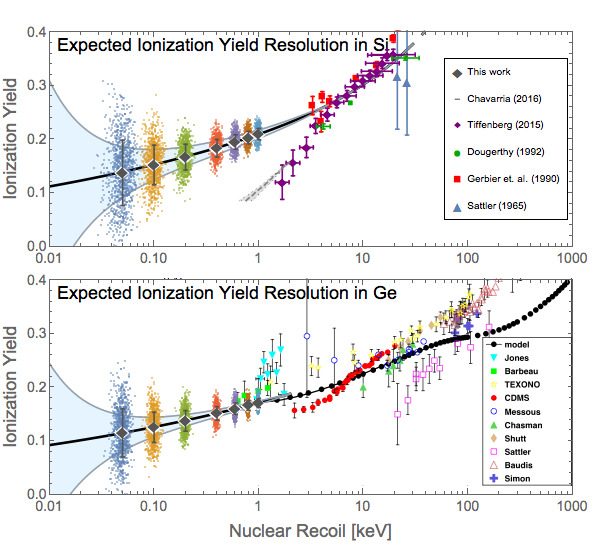
\includegraphics[width=0.75\textwidth, trim={0 0 0 20}, clip]{Figures/Yield_Baseline_vs_Literature_SiGe}
\caption{Comparison of a simulation of the proposed ionization yield measurement compared with existing measurements of the mean ionization yield from the literature. The proposed measurement, shown following a Lindhart ionization yield model, has the potential to provide essential data on the ionization yield mean and statistical fluctuations for dark matter rate calculations in the lowest energy ranges. 
The colored scatter points correspond to the simulated ionization yield as a function of recoil energy, superimposed on the \(\pm1\sigma\) statistical uncertainty band from Eq.~\ref{eq:yielderr} (note that the blue \(\pm1\sigma\) bands only account for the statistical uncertainty due to phonon energy resolution and neutron scattering angle, whereas the actual points also include the effect of electron-hole production statistics, i.e., the Fano Factor). The gray diamonds indicate the mean value of the calculated yield from the simulation, and the vertical bars are the square root of the variance. Figure adapted from~\cite{2013APh....48....8B,1965PhRv..138.1815S,1990PhRvD..42.3211G}.
%\vspace{-3ex}
}
\label{fig:exp_vs_litt}
\end{figure}
Figure~\ref{fig:exp_vs_litt} shows current mean ionization yield measurements in germanium and silicon detectors made with a variety of detector technologies, along with the theoretical prediction from the Lindhard model~\cite{1964PhL....12..126L}. Also shown (and discussed fully in the subsequent sections) are a set of simulated yield measurements %done by the \UF group
demonstrating what would be possible with the proposed work, superimposed on the current state of knowledge of the low energy nuclear recoil yield in germanium~\cite{2013APh....48....8B} and silicon~\cite{1965PhRv..138.1815S,1990PhRvD..42.3211G,1992PhRvA..45.2104D,Chavarria:2016arXiv}. Highlighting the importance of experimental data, a recent measurement, made by the DAMIC collaboration (top panel of Figure~\ref{fig:exp_vs_litt}), indicates that the ionization yield in Si is significantly different from the theoretical predictions of Lindhard at and below 1\keV.  Projecting the deviations down to 100\eV suggests even larger discrepancies.

For SuperCDMS, the interplay of ionization yield, trigger threshold and experimental sensitivity is complex.  As the ionization signal is detected via its conversion to phonons by the Luke-Neganov effect, the total phonon signal measured includes both primary phonons from the recoil and Luke-Neganov phonons from primary ionization. In Figure~\ref{fig:SensitivityYVScanHV}, calculations for Si show how the sensitivity can vary with different ionization yield assumptions.  Furthermore, systematic bias from uncertainty in the ionization yield can be reduced and sensitivity to the lowest masses regained by operating at reduced voltage at the cost of higher background in the signal region (as demonstrated by the extreme case of 0\,V, which is used here to show the theoretical maximum effect).  Both issues demonstrate the need to measure the ionization yield of \scdmssnolab HV detectors by the time science runs at \cute begin.
\begin{figure}[htp]
\centering
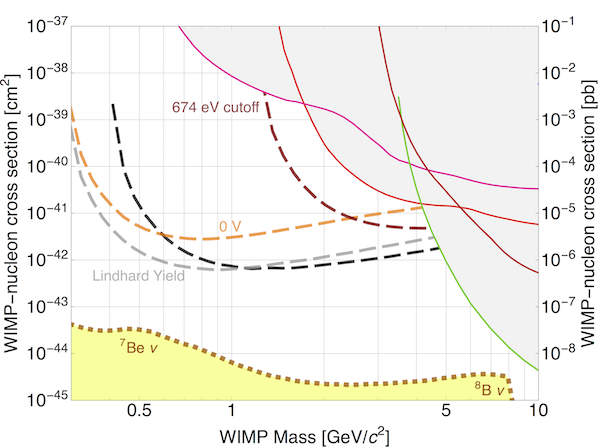
\includegraphics[width=0.48\textwidth]{Figures/Sensitivity_Si_YV_Scan}
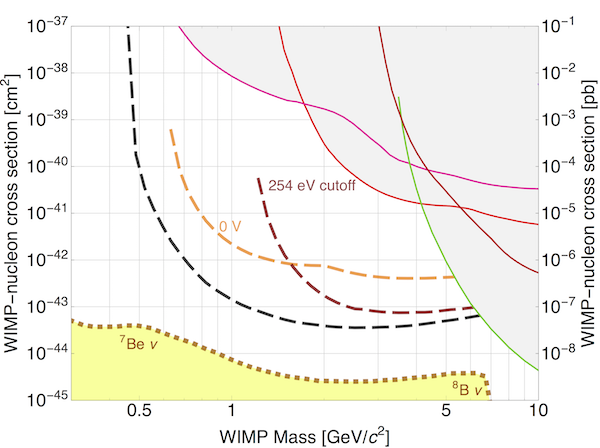
\includegraphics[width=0.48\textwidth]{Figures/Sensitivity_Ge_YV_Scan}
\caption{Left panel: Sensitivity scan of SuperCDMS SNOLAB Si HV detectors for different yield and analysis thresholds. Black is the nominal projected sensitivity, which uses the DAMIC yield function~\cite{Chavarria:2016arXiv} and extrapolates the yield curve down to 40\,eV~\cite{SuperCDMSSensitvitiy:2016arXiv}. Grey is Lindhard theory for comparison. Orange is the sensitivity projection for operation of the detector with zero voltage across the crystal. The red line shows the sensitivity from an analysis that sets the threshold at the lowest recoil energy for which data on ionization yield exists (675\,eV). The region to the left of the red line highlights the WIMP parameter space that requires new experimental data for ionization-measuring detectors. Right panel: Same as Left but for Ge HV. The black line uses Lindhard theory, orange is zero-voltage operation, and red applies an analysis threshold of 254\,eV.
%\vspace{-3ex}
}
\label{fig:SensitivityYVScanHV}
\end{figure}

\subsubsection{Measurement Strategy}

We propose to perform a precision measurement of the ionization yield in this energy range first at a neutron beam facility with small prototype detectors and subsequently using a D--D neutron generator with full-sized SuperCDMS SNOLAB detectors.  In both these setups, the energy of the incoming neutron is known and the deposited nuclear recoil energy in the detector is determined kinematically by measuring the outgoing neutron angle. By directly measuring the ionization signal in the target/detector it is then possible to perform a direct measurement of the ionization yield. 

%%%%%%%%%%\subsubsection{The Voltage-Assisted Calorimetric Ionization Detection Technique}
\SuperCDMS detectors determine the properties of a particle interaction by measuring the energy deposited in two different physical channels: the phonon and ionization channels. When an interaction takes place in the detector the total recoil energy of an interaction is initially divided among a population of prompt athermal phonons and a population of charged excitations (\textit{i.e.}, electrons and holes). A uniform electric field of a few V/\(\!cm\) causes the electrons and holes to drift to opposite surfaces where they are detected with a capacitively-coupled charge amplifier. The motion of the charged excitations in the crystal under the influence of the applied electric field creates a population of phonons known as Luke-Neganov phonons. These release to the phonon system an amount of energy equal to the work required to drift the charges through the field across the resistive crystal, i.e., $E_{Luke} = n_{eh}\,e\,V$, where $n_{eh}$ is the number of electron hole pairs made in the recoil, and $e\,V$ is the electron charge times the voltage across the crystal.  The total phonon energy $E_{ph}$ measured in the detector for a given recoil energy $E_r$ is,
\begin{equation}
\label{eq:yield}
E_{ph} = Er + E_{Luke} = E_r \left ( 1+\frac{e\,V\,Y}{\mathcal{E}_{eh}} \right )
\end{equation}
where $\mathcal{E}_{eh}$ is the average electron equivalent energy required to form an electron hole pair, $Y$ is the ionization yield

Effective ionization resolutions on the order of few eV (corresponding to individual e-h pairs) can be achieved using the technique of voltage-assisted calorimetric ionization detection which was first used by the \SuperCDMS experiment in a low-mass WIMP search using the current iZIP detectors~\cite{2014PhRvL.112d1302A,Agnese:2015nto}. By applying a high voltage (HV) across the crystal the ionization signal can be effectively amplified and measured using the phonon sensors since the energy released into the Luke-Neganov phonon population will dwarf the intrinsic recoil phonons. The detector is then being effectively operated as a phonon-based charge amplifier in which the gain of the signal is proportional to the applied voltage, and the readout channel has a fixed resolution.  The measurement uncertainty of the ionization yield, measured using Eq.~\ref{eq:yield} , the measured total phonon energy and an independent determination of the recoil energy (\textit{e.g}., from a neutron scattering angle measurement), is: 
\begin{equation}
\sigma_y= \frac{\mathcal{E}_{eh}}{e\,V}\frac{\sqrt{E_{rec}^2\sigma_{ph}^2+E_{ph}^2\sigma_{rec}^2}}{E_{rec}^2}
\label{eq:yielderr}
\end{equation}
Since the ionization yield uncertainty depends both on the phonon channel resolution and the bias voltage, a worse than expected phonon resolution can be compensated for with a higher voltage bias. %Above a bias of 500\volt , however, the uncertainty becomes dominated by the uncertainty in the recoil energy (from the event kinematics measurement), taken to be 100\eV in this calculation.

Figure~\ref{fig:exp_vs_litt} shows the result of a simulation % by the \UF group, 
with neutrons incident on a test detector with 50\eV resolution, superimposed on the current state of knowledge of the low energy nuclear recoil yield in germanium~\cite{2013APh....48....8B} and silicon~\cite{1965PhRv..138.1815S,1990PhRvD..42.3211G,1992PhRvA..45.2104D,Chavarria:2016arXiv}. This simulation shows that this experiment will have the ability to reliably identify the mean value of the ionization yield down to \(\sim 50\eV\). The horizontal spread in each population of events arises from a given neutron detector accepting a \(\pm 1\deg\) range of scattering angles.

At the improved, but still conservative, energy resolution of 10\eV (this value is twice the expected 5\eV resolution of the \SuperCDMS R\&D devices that will be used for the measurement) it becomes possible to identify the number of electron-hole pairs produced by a given recoil as shown in Figure~\ref{fig:eh_counting}. This will provide an important piece of information regarding the statistical nature of ionization production and allow us to perform a direct measurement of the Fano factor down to the lowest recoil energies.

\MP{include quantization plot from Stanford.  Switch plots to show quantized sensitivities}

\begin{figure}[t]
\centering
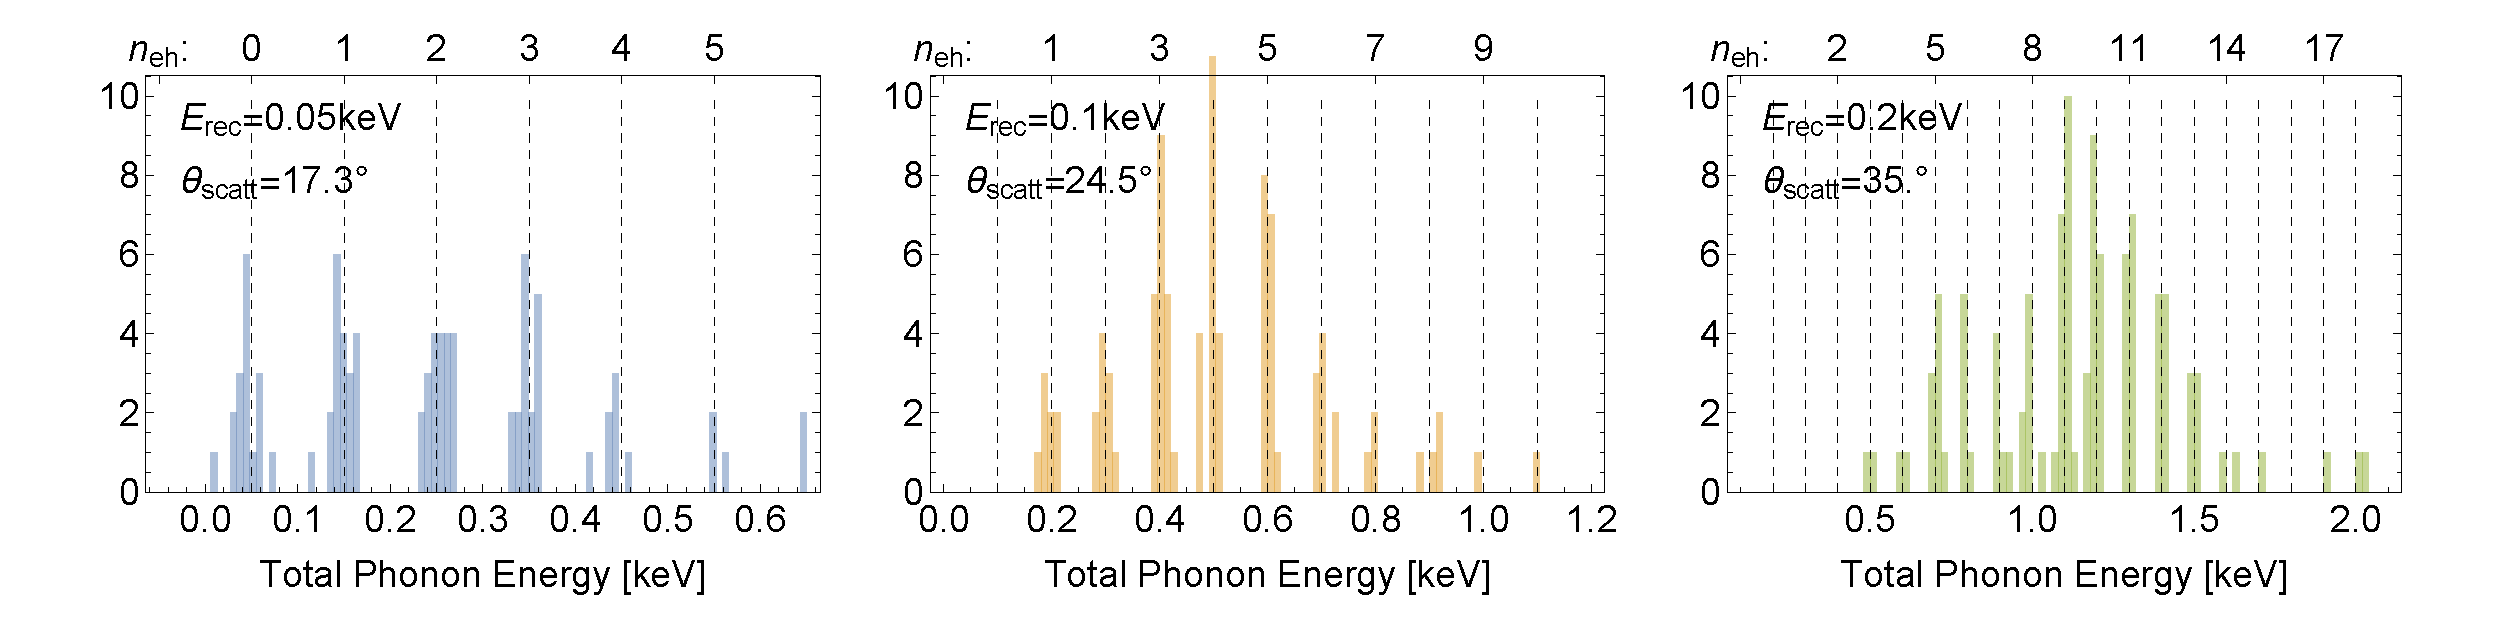
\includegraphics[width=\textwidth]{Figures/Phtot-Hist-Neutron-beam-HiRes-G4}
\caption{
Demonstration of the ability to identify the number of discrete electron-hole pairs (indicated by the dashed vertical lines) created by a low energy nuclear recoil. The combination of high bias voltage and excellent energy resolution allows for the measurement of the Fano factor even with limited statistics.
%The figure is based on simulations performed by the \UF group.
%\vspace{-2ex}
}
\label{fig:eh_counting}
\end{figure}

\subsubsection{Yield Calibration with a Neutron Beam at TUNL (\WBS 1.1.1)}
\label{sec:tunl}

The Triangle Universities Nuclear Lab (\tunl) data taking campaign will occur in the first year of this grant (see schedule in Figure~\ref{fig:ops-schedule}). \tunl operates a facility capable of delivering a mono-energetic neutron beam with energies in the range of 30\keV to a few\MeV~\cite{TUNL:website,Theprecisionquench:2014tw}. A tandem Van de Graaff is used to accelerate protons and collide them with a \isotope[7]{Li} target. The resulting \isotope[7]{Li}(p,n)\isotope[7]{Be} reaction produces a neutron that is primarily collinear with the proton beam. At a proton threshold energy of 1.88\MeV the reaction produces neutrons with 29.7\keV kinetic energy which are kinematically constrained to be in the forward direction. Increasing the proton energy allows for the production of neutrons with a range of kinetic energies and directions, however by selecting a particular direction (e.g. collinear with the proton beam) a unique neutron energy is obtained~\cite{1999NIMPB.152....1L}.

The neutron beam passes through a 2 foot high-density polyethylene (HDPE) block which collimates the beam and absorbs unwanted reaction products (such a \(\gamma\)-rays) and is directed to the target location. Backing detectors  (5cm inch diameter plastic scintillator, with sensitivity to neutrons down to 6\keV) surround the interaction site and detect the scattered neutron providing knowledge of the scattering angle and timing of the event, and can be positioned around the interaction point as needed. The TUNL facility currently has 32 such detectors and is in the process of deploying 200 more to provide a solid angular coverage of almost \(1\pi\) steradian. The additional neutron detectors are expected to become available in January of 2017. One of the most useful features of the facility is its ability of providing a pulsed beam, which in conjunction with the backing detectors' timing resolution of \(< 4\,\)ns allows for an excellent rejection of events due to pileup, multiple scatter or radioactive backgrounds, and also provides a secondary measure of the neutron energy through its time-of-flight.

The details of the backing detector configuration will be investigated and optimized in the early stages of the proposed work plan in order to obtain an experimental setup that allows for making the measurement at the the desired level of accuracy in a minimum amount of beam time.

%%%%%%%%%%\subsubsection{Calibration at a Neutron Beam Facility}
%Calibration at a neutron beam facility, such as TUNL~\cite{TUNL:website}, is attractive because the beam energy can be tuned as low as $\sim$30\keV and an extensive secondary neutron detector array is available for use~\cite{Theprecisionquench:2014tw}. 
The Northwestern \SuperCDMS group owns an Adiabatic Demagnetization Refrigerator (ADR) that can be transported to TUNL to perform such a measurement.  The ADR can cool small, special-purpose Ge and Si HV detectors, each with mass of a few grams. Detectors of this size are produced as part of the \SuperCDMS R\&D program and are available for these measurements. Two such detectors (one made of Si, one of Ge) will be installed in the ADR so the \tunl measurements can be done without warming up or opening the cryostat.

The kinematics at a neutron beam result in an excellent recoil energy resolution: for a \(1\deg\) uncertainty in the direction of the scattered neutron, the reconstructed energy resolution is on the order of 4\eV for a 100\eV recoil. This value is close the the expected 5\eV resolution of the \SuperCDMS phonon sensors, and as seen in equation~\ref{eq:yielderr}, is optimal for achieving excellent ionization yield resolution. The neutron beam measurements will be used to obtain the highest resolution ionization yield measurements at the lowest energies allowing us to study in detail the physics and statistics of electron-hole pair production via nuclear recoils at their creation threshold.


\subsubsection{The TUNL Experimental Campaign}

The simulation in Figure~\ref{fig:exp_vs_litt} assumed \(10^3\) events for each recoil energy. We investigated a feasable set of operational parameters necessary for obtaining such statistics in the actual data while minimizing the amount of multiple scatter, pileup and background events in the data. The two driving variables are the detector response time, and the interaction probability of a neutron with the detector. 

Based on a conservative detector recovery time of \(\tau=1ms\) we wish to keep the interaction rate in the detector below 100~Hz to minimize pulse pileup. The mean free path of 30\keV neutrons in silicon (germanium) is \(\sim 2cm\) (\(\sim 2.3cm\)), which gives a 18\% (16\%) probability for a single neutron to interact in the 4mm thick test detector. This can lead to a large number of simultaneous interactions in the detector from a single beam pulse contaminating the data. This effect can be mitigated by decreasing the average number of neutrons per beam bunch. A mean number of neutrons per bunch of \(n_{mean}=0.4\) results in less than 3\% contamination from simultaneous interactions. The combination of \(n_{mean}=0.4\) and a bunch frequency of \(\frac{1}{600\mu s}\) results in a net detector interaction rate of 100~Hz. Such an operating mode is well within the capabilities of the facility and given the $< 4$~ns timing resolution of the backing detectors there will be no difficulties distinguishing which beam bunch produced a particular interaction~\cite{barbeau:2014}. Assuming that each backing detector covers an angle of \(\left( 1\deg\right)^2\), that they are positioned in groups of 10 at each of 20 angles, and that the net neutron interaction rate in the detector is 100~Hz, we can estimate the total active beam time required to obtain the necessary statistics to be around 12 hours. The data for the different recoil energies is collected simultaneously by the grid of \(>200\) backing detectors at 20 specific scattering angles. Assuming a net efficiency of five to six hours of beam time per calendar day, it is reasonable to expect that a data acquisition period of a few days is sufficient for a particular measurement. Data will be taken for both a prototype Si and Ge detector, at multiple bias voltages and operating conditions (such as crystal temperature) during a three week running window. An additional week before and after the data acquisition campaign for assembly/disassembly and verifying the operation of the detector at the TUNL facility will also be required.

\subsubsection{Data Contamination}
\begin{figure}[tb]
\centering
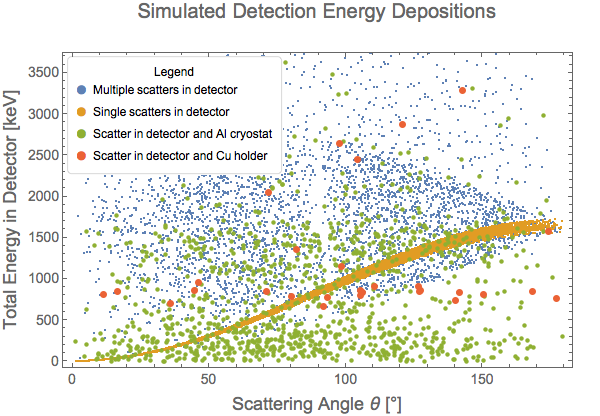
\includegraphics[width=0.45\hsize]{Figures/single_multiple_scatters_geant}
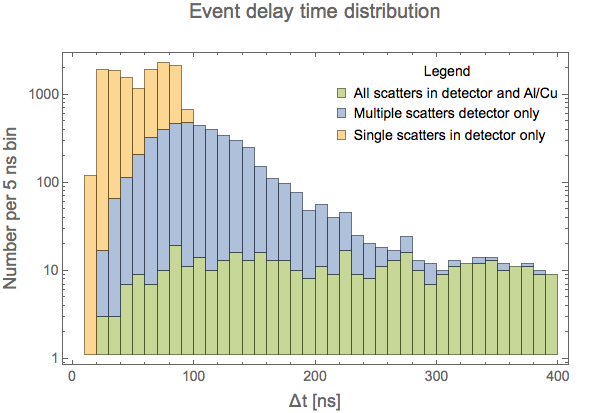
\includegraphics[width=0.45\hsize]{Figures/Delta_t_histograms}
\caption{Left panel: %Distribution of 
Energy deposited in the detector as a function of neutron scattering angle. The orange band band represents events in which the neutron scattered only once within the detector without interacting with the surrounding material. Events which multiply scatter within the detector are shown in blue, and events which interact with the Al or Cu surrounding the detector are shown in green and red respectively. Right panel: Histogram of the event delay times, i.e. the time between the arrival of a beam bunch and the detection of a neutron in the backing detectors. The delay was defined such that \(\Delta t=0\) for a non-scattered neutron, and the backing detectors' timing resolution is \(< 4\,\)ns.
\vspace{-3ex}
}
\label{fig:geant}
\end{figure}

Environmental radiation background and neutron interactions with the material surrounding the detectors have the potential to contaminate the data. A proper understanding of these interactions requires a detailed Monte-Carlo simulation. The results from a basic \geant simulation done by our U. Florida collaborators and shown in Figure~\ref{fig:geant} are still quite informative. They simulated the interactions of a neutron beam with a detector surrounded by a 1mm thick copper housing, contained in a 1cm thick aluminum cylindrical shell (which represents the cryostats vacuum jacket). The figure's left panel shows the distribution of energy deposited in the detector as a function of neutron scattering angle. The thick orange band represents events in which the neutron scattered only once within the detector without interacting with the surrounding material.  Multiple scatters within a detector, as well as events in which the neutron interacts with the surrounding material are also shown. The right panel shows the delay time distribution (the time between the arrival of a beam bunch and the detection of a neutron in the backing detectors). It can be seen that a time based acceptance cut can remove a large portion of multiply scattered events and interactions in the surrounding material. It is worth noting however, that even without applying any selection criteria, the simulation shows that contamination from such events is less than 5\% for all recoil energies \(< 1\keV\).



\subsubsection{D-D Generator Measurements at NEXUS (\WBS 1.1.2)}
\label{sec:ddcal}

\MP{What about testing the concept of measuring nuclear recoil ionization yields with Cf by measuring 0V, 50V, 100V. This would give us the possibility of using Cf for insitu calibration of all detectors in SNOLAB (or at NEXUS) extremely easily}

There are several challenges associated with calibrating large cryogenic solid-state detectors in a fixed neutron beam.  These massive detectors require a dilution refrigerator to operate at millikelvin temperatures, and such refrigerators are not portable.  Adiabatic Demagnetization Refrigerators, although portable, lack the cooling capacity to effectively operate these detectors. Furthermore, underground calibrations are critical for large cryogenic detectors. When operated on the surface, the time between events from cosmic radiation can be less than the recovery time required for the phonon sensors to return to equilibrium. \MP{this just isn't true. We have a compton background of 40Hz (25ms) and a falltime which is <100us ... we have 250 falltimes on average between comptons. The bigger problem is muons [perhaps what you were referring to] ... muons occur @1Hz and have a 200ms thermal falltime.  We find that with a muon cut with 50\% passage, we get rid of this to the point that it's subdominant to other noise sources ... it's definitely a penalty (50\% livetime) ... but it's not a true deal breaker ... remember that the livetime of our old DAQ was only 15\%. We still take more good data now with the muon cut then we ever took with the old DAQ at UCB)}.

The portability of a D--D generator allows for neutron calibration at underground locations, such as \nexus, described in Section~\ref{sec:nexus}. 

%MOVED to NEXUS section
%\begin{figure}[t]
%\centering
%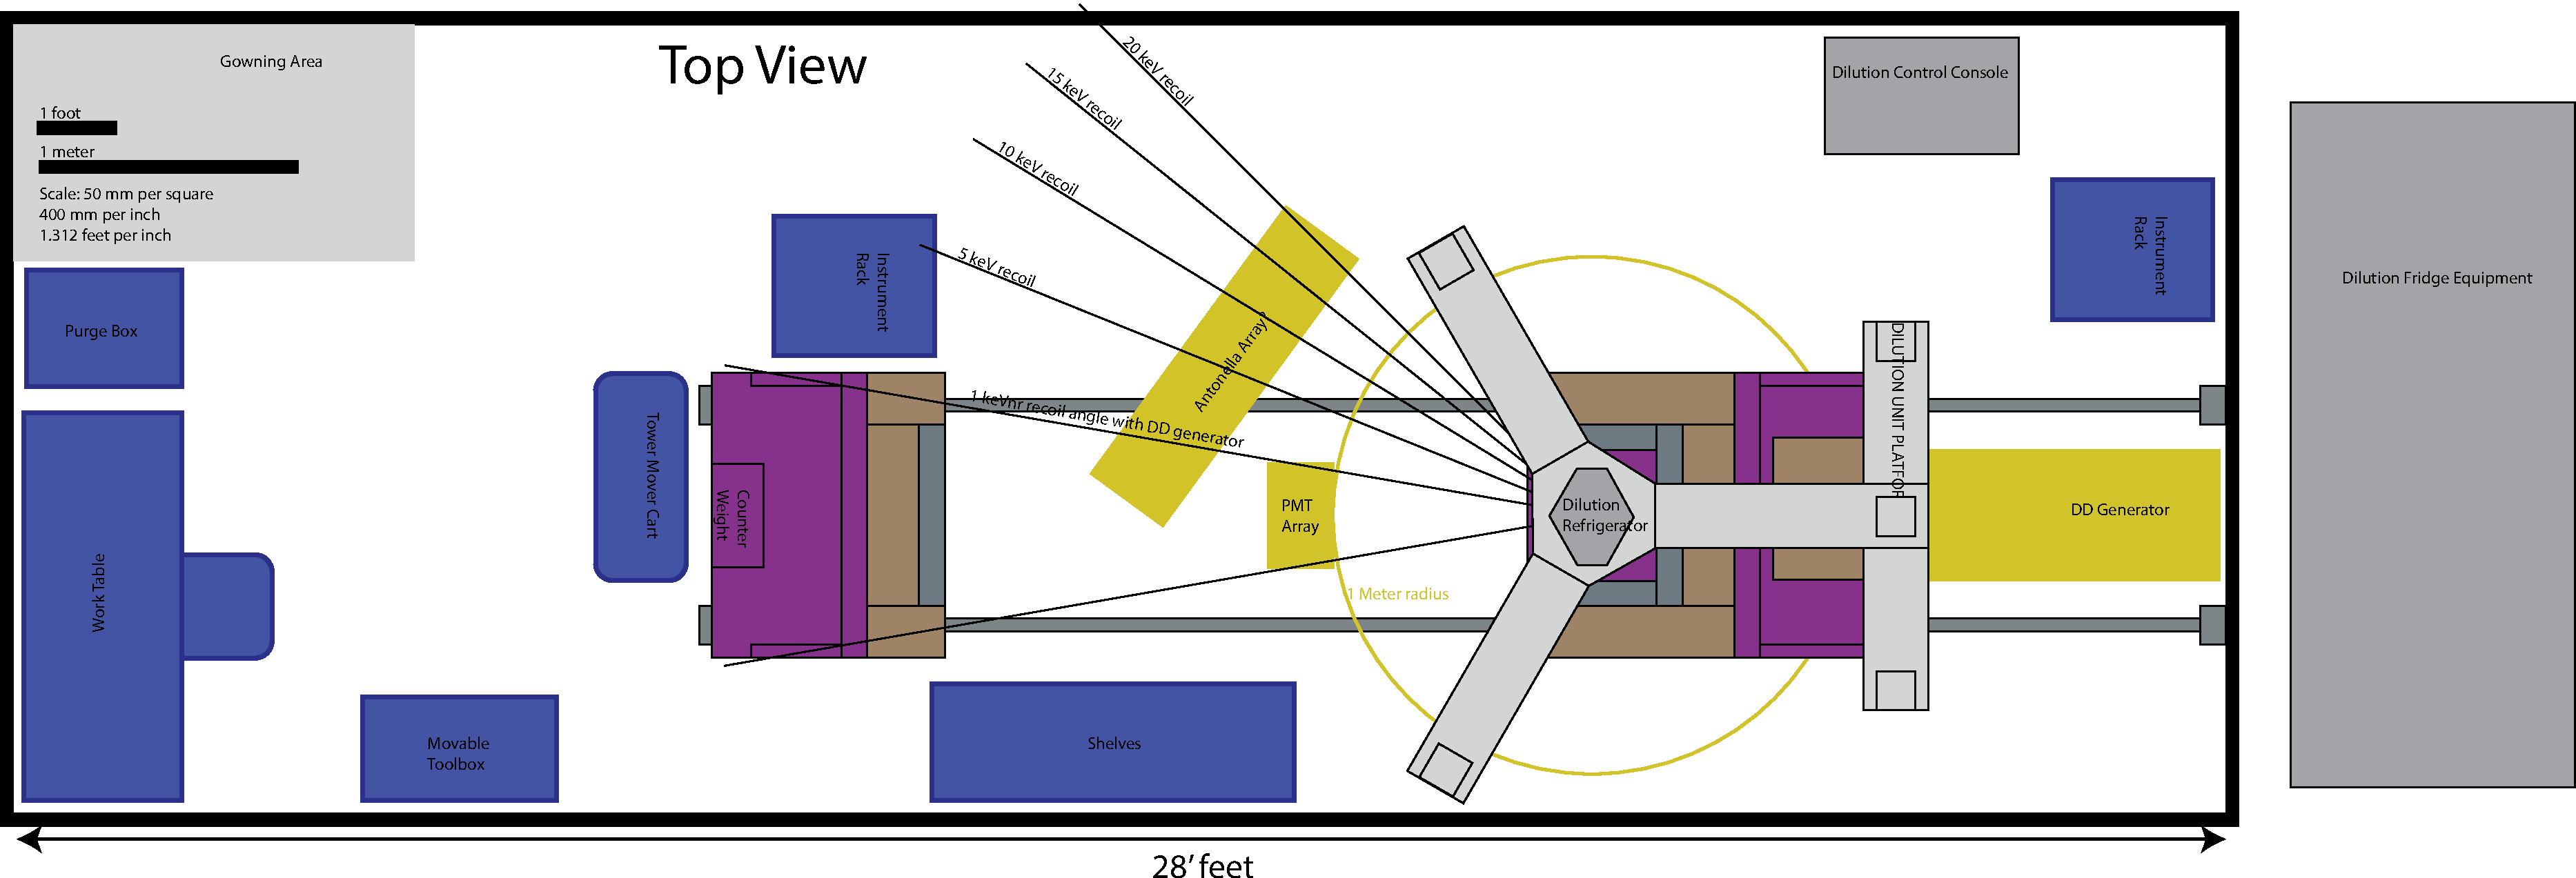
\includegraphics[width=\textwidth]{Figures/NEXUS-Layout-YieldMeas}
%\caption{\nexus layout schematic. The outer box delineates the clean room to be placed 100 m underground in the \numi access tunnel. The blue boxes are support equipment, while the grey, brown, and purple structures are the passive shield, which is on rollers and half of it is moved out to the left to allow the neutron backing detectors to be placed. The D--D generator is shown as a yellow box on the right, with neutrons passing through a collimating hole in the shield toward the detectors. Neutrons hit the HV detectors in the dilution refrigerator and scatter into angles as labeled depending on the recoil energy. An existing array from Fermilab will cover the wider angles between up to 20~keV, while a purpose-made fine-grain neutron detector PMT array will cover the recoil energies below 1~keV.\vspace{-2ex}}
%\label{fig:nexus}
%\end{figure}


Calibration with a D-D generator requires borated poly shielding to collimate the D-D neutrons into a beam and a moderate amount of lead shielding to block the capture gammas. Additionally, secondary neutron detectors are needed to measure the scattered neutrons at a given angle.  The ANTONELLA collaboration has a neutron detector array, that was created exactly for this purpose and is currently available for use.  This array covers relatively large angles of scatter ($>$10$^\circ$).  With this array, we can measure nuclear recoils down to a few keV with the D-D beam energies.  Measurement down to 100 eV requires fabrication of a finer-grained neutron array. Design of such an array, with the reuse of 1.3 cm Hamamatsu photomultiplier tubes salvaged from the SELEX experiment, will be pursued by the U. Florida and Fermilab groups. The setup is schematically shown in Figure~\ref{fig:nexus}.

\MP{Has this array been procured?  If not then you are just doing nuclear recoil ionization yield measurements @ a few keV}

In \SuperCDMS detectors, there are energy-scale effects that are degenerate with measurement of the ionization yield and can vary with detector parameters such as the strength of the electric field, fabrication of the phonon sensors, and even the impurity levels in a given crystal.  To understand these systematic effects, it is important to perform the calibration on detectors that will have the same electric field and style of phonon sensor.  Furthermore, it is highly desirable to perform measurements on several different detectors of the same type, operated at several bias voltages.  \MP{explain} 

The primary challenge of the D--D calibration is the relatively high energy (2.5\MeV) of the neutrons compared to the recoil energies of interest (100\eV). For a \(1\deg\) uncertainty in the direction of the scattered neutron the reconstructed energy resolution of a 100\eV recoil becomes \(\sim 30\eV\). This uncertainty becomes the limiting factor in the measured yield resolution. One way to compensate for this effect is to use a fine-grained neutron array to determine the neutrons' very small scattering angles. An angular resolution of \(\sim0.125\deg\) is needed to achieve the same recoil energy resolution as with the 30\keV\ \tunl neutron beam. The resulting scattering rates per secondary neutron channel will be approximately 60 times lower compared to the rates at a neutron beam facility. The lower detection rates, in turn, lead to longer data acquisition times and an increased sensitivity to environmental backgrounds. Studies will optimize the tradeoff between recoil energy resolution and the impact of data contamination sources such as background interactions in the neutron array and multiple scattering of the D--D neutrons both within the \SuperCDMS detectors and the surrounding material of the dilution refrigerator. 

The neutron beam and D--D setups will experience different experimental systematic effects.  By taking data with the small calibration detectors at the D--D generator setup, we can correlate the neutron beam and D--D systematics, and use this understanding to extrapolate the high-resolution beam data to the kg-size detectors.  Thus a cross-calibration would provide robustness to our understanding of the ionization yield and provide additional higher-resolution data points in the energy region where currently no data exists. The data with the small HV detectors at \nexus will be taken in the latter part of Year 1 of this grant. Year 2 of the grant will be devoted to pre-production \scs detector calibration (see schedule in Figure~\ref{fig:ops-schedule}).
%We will also investigate the possibility of operating at the same angular resolution as that of the TUNL facility (\(1\deg\)), and using the information from Monte-Carlo simulations and the TUNL measurements to extract high resolution ionization yield information at low energies from the D--D measurement.

The D--D calibration setup will enable a program of measurements that can explore the calibration differences that arise with different operating conditions and detector designs.  This will lead to a full understanding of the systematic uncertainties associated with ionization production in \SuperCDMS detectors. 

%Summary
In summary, the \tunl \& \nexus campaigns enable a program of measurements that can obtain high-resolution physics measurements of the ionization yield of Si and Ge at recoil energies down to 100~eV and below, explore and correct for systematics in the measurements, and perform direct measurements of the ionization yield of \scs detectors.  This will enable a full understanding of the systematic uncertainties and provide essential inputs for the dark matter science analysis of \scs data.


%%%%%%%%%%%%%%%%%%%%%%%%%%%%%%%%%
\subsection{Detector Performance Characterization and Background Studies (\WBS 1.2)}

\MP{
\begin{itemize}
	\item Nuclear Recoil Ionization Yield Measurement
    \item testing optical photon calibration techniques
    \item Charge Leakage Studies
    	\begin{itemize}
        	\item optimize pre-bias voltage
            \item optimize LED/blackbody frequency for A+,D- 
            \item optimize bias voltage
        \end{itemize}
    \item Electronic Recoil / Nuclear Recoil Discrimination
    	\begin{itemize}
        	\item Quantization / Statistical subtraction in HV 
            \item Standard ER/NR in iZIP
        \end{itemize}
    \item Fiducialization Metrics 
    \item (@ Berkeley) noise studies with small TES chips
\end{itemize}
}

The \MP{Nuclear Recoil / Electron Recoil?} discrimination power and general behavior of \scs detectors under low-background conditions cannot be tested in regular detector test facilities due to the high rate of cosmic ray induced interactions in the detectors. A large focus of this proposal is to make such measurements at \nexus and \cute. 

\MP{why not discuss charge leakage optimization specifically?}

\subsubsection{Detector Characterization with NEXUS}

Although the nuclear recoil energy calibration (described in detail in section~\ref{sec:calibration}) will be the main focus at \nexus, having pre-production detectors at the site will also allow early detector characterization. The  ability to kinematically reconstruct nuclear recoil energies, as well as the flexiblity to place and remove gamma sources, will faciliate studies that impact the analysis and interpretation of the \scs data. 

\MP{these are all really important ... they should have similar size at the nuclear recoil ionization yield work if possible}
These include position dependence and specific detector Monte-Carlo tuning studies (see Section~\ref{sec:dmc}), voltage bias scan studies, and other studies such as measuring single electron-hole pair production using optical fibers. 
The goal of the optical fiber studies will be to directly measure the separation between integer numbers of electron hole pairs near the threshold of HV detectors as a means to confirm the electron recoil energy scale near threshold.  The optical fiber setup also allows for studies of charge collection, which could inform operating procedures for the main experiment. These measurements will take place during Year 2 of this proposal, at the end of each detector's calibration measurement. 

\subsubsection{Background Studies and Precommissioning with CUTE}
\label{sec:CUTE}

A primary goal in the design of the \cute facility is to test the capability of the \SuperCDMS HV and iZIP detectors to distinguish surface from bulk events (fiducialization). The discrimination power between electron and nuclear recoils of the \SuperCDMS iZIP detectors can also be studied in detail. Additionally, functionality and early commissioning checks of a tower can be performed before it is deployed within the main \SuperCDMS cryostat.  Functionality checks would verify that electrical and thermal connections in the tower are functioning properly after shipment to \SNOLAB. Early commissioning checks include optimization of voltage bias and neutralization studies.  These tests are best performed in a low-background installation such as \cute because breakdown voltage and optimal neutralization conditions have previously been found to  correlate with event rate.

Recent measurements of detectors used for \SuperCDMS \Soudan have shown that the noise in the signal region increases linearly with the applied bias voltage. Such behavior would limit the sensitivity of the new \SuperCDMS HV detectors that are designed for operation with up to 100~V bias. The origin of this excess noise is not yet fully understood. Possible explanations include infrared leakage and injection of charges through the contacts. Low-angle Compton scattering has been identified as alternative explanation; this would also explain why the observed noise level appears to be the same in different test facilities with no, or only moderate, shielding.

\MP{where did this theory come from? ... why would there be a huge number (1e5Hz) of single e/h pair comptons?}

We will test this hypothesis and understand the behavior of the new \SuperCDMS HV detectors in \cute's low background environment.

As shown in the schedule (Figure~\ref{fig:ops-schedule}) we expect to install in \cute one of the two pre-production towers at the beginning of calendar 2018 after the tests planned by the \scs Project are finished. This tower is intended to have two pre-production HV detectors and one pre-production iZIP.

After 2 months of commissioning and basic checks of performance, we plan a 9-month testing program to study:
\begin{compactitem}
\item  Fiducialization and surface rejection in HV detectors.
\item  Nuclear recoil discrimination of iZIP detectors.   
\end{compactitem}

\subsubsection{Detector Monte-Carlo Validation}
\label{sec:dmc}

The \SuperCDMS collaboration is currently in the process of building a \geant based detector Monte-Carlo that incorporates low-temperature ionization and phonon physical processes governing the behavior of electrons, holes, and phonons in the \SuperCDMS detectors. The physical processes being added to \geant include:
\begin{compactitem}
\item A microscopic model of inter-valley scattering for charge charge carriers in the crystal.
\item Luke-Neganov phonon emission based on the charge carrier mean free path in a varying electric field.
\item A continuous process of phonon impurity scattering.
\item The creation and tracking of quasiparticles in the the Al superconducting films that at part of the phonon sensors.
\item Differential equation based models of the FET (ionization sensor readout) and TES (phonon sensor readout) responses.
\end{compactitem}

Data from the \tunl and \nexus campaigns will consist of a set of nuclear recoil events with well defined kinematics.  Additionally, the data obtained  from the precommissioning calibration at \cute will provide a large set of events from gamma and neutron calibration sources taken in a low background environment. 
These data sets will provide a comprehensive collection of events for comparing against Monte-Carlo simulations. The data will be made available to members of the \SuperCDMS collaboration who are working on detector Monte-Carlo and simulation activities and are validating the performance of the detector Monte-Carlo, and refining it in preparation for the \scs experiment. %Funding for such work, however, is not part of this proposal.

%%%%%%%%%%%%%%%%%%%%%%%%%%%
\subsection{Early \scs Science (\WBS 1.3)}

One of the attractive features of the plan we propose for \cute is that it not only will give us the opportunity to exercise our detectors in a low background environment but that it might allow us to get early science results.
While the characterization of the pre-production detectors described in \ref{sec:cute} is taking place in calendar 2018, the \scs Project is scheduled to complete the first production HV tower.  We are proposing to install this first tower in \cute at the beginning of 2019 (Figure~\ref{fig:ops-schedule}). This tower would have 6 HV detectors, with a mix of Germanium and Silicon.  
Our first goals will be to:
\begin{compactitem}
\item  Assess the performance of these detectors in a realistic environment (voltage limits, leakage current, background level)
\item  Develop biasing schemes for the HV detectors
\item  Learn what small detector or cold hardware modifications we could include in the second HV tower, being produced in 2019, to optimize its performance
\item Exercise our data acquisition system, optimize our reconstruction software and begin to develop the algorithms for science analysis
\end{compactitem}

Achievement of these goals would be very beneficial to the subsequent commissioning of the \scs experiment. If all goes well, there is a reasonable prospect for doing early science with the HV tower in \cute, which is the main justification for  installing the additional lead shield that we propose to acquire in this award. Current simulations indicate that we could decrease the gamma background from 30 events/kg/keV/day to about 2 events/kg/keV/day with the additional lead shielding. In that case, a six-month HV tower run at \cute, with a baseline phonon resolution of 10 eV r.m.s. and 100 V bias (\scs goal) and the projected $^3$H and $^{32}$Si levels for \scs, might give a spin independent sensitivity as much as 4 orders of magnitude better than the current best limit \cite{2012EPJC...72.1971A} at a dark matter mass of 2 GeV/c$^2$ with Germanium, roughly a year before our first results from the \scs experiment will become available. 
%The improvement could be as large as a factor 2000 at 1 GeV/c$^2$  with our Silicon detectors. This would be only 20 times worse than the first result that we should obtain at \scs for Germanium with optimal interval method \cite{Yellin:2002xd} and about a factor six times worse for Silicon, if the $^32$Si is at the level indicated by DAMIC for a bulk contamination.  

Of course, \scs will then go on to produce much better sensitivity and reach to even lower mass. The two iZIP towers that will be included in the first \scs payload will provide an independent measurement of the background, which should yield an additional factor of 5 in sensitivity over the no-background-subtraction projections in~\cite{SuperCDMSSensitvitiy:2016arXiv}. Moreover, the second HV tower planned for the first \scs payload will have benefited from the experience of the first tower at \cute and is likely to perform better. In the long run, the \scs set up is designed to allow us to reach the neutrino floor, well beyond what will ever be possible at \cute.
Still, the potential sensitivity of a run of the first HV tower at \cute is an exciting science opportunity and will provide theses for our graduate students and interesting publications to further the career of our younger scientists.

%%%%%%%%%%%%%%%%%%%%%%%%%%%
\subsection{\scs Commissioning (\WBS 1.4) }

The \scs Project will include acceptance tests of all parts of the experimental apparatus at the surface. The Project objective is to complete the  installation of all equipment underground at \SNOLAB, although the Project threshold does not require this. \scs Operations will pick up any remaining installation tasks, then commission the experiment and transition to operations. We expect this period to occupy approximately the last six months of this proposal's performance period.

The commissioning period will be a mix of installation and testing of subsystems, followed by system testing and data runs that exercise the full experiment. System experts will be responsible for testing and documenting their equipment, with work coordinated by an on-site commissioning czar. The initial focus will be on the cryogenics system, since a successful cool down of the experiment to base temperature is required before detector tower commissioning is possible. In parallel, the readout electronics, data acquisition/trigger and software chain can be exercised. Once base temperature has been established, the focus will shift to commissioning the detector towers, using gamma and neutron sources for calibration. iZIP and HV detector towers will be studied in parallel, and the electronic noise and vibration environment will be characterized. 

As system commissioning matures, the operations manager and operations team will begin to take overnight data runs and examine the data along with the commissioning czar and system experts, to find any subtle problems. The data quality monitoring system will be commissioned, as well as the data pipeline and processing systems. Towards the end of commissioning period, we will be running most of the time, with scheduled down times to fix any problems that have been identified. During this period, the operations documentation needs to be finalized.  

NSF-funded scientists will play key roles in commissioning, with a special focus on areas covered by this proposal, especially detector performance and  calibration.  Data from pre-operations studies will be extremely useful in making sure that commissioning is smooth and that the experiment can begin taking dark matter search data as quickly as possible.

%\clearpage

% !TEX root = NSF_SuperCDMS_SNOLAB_OPS.tex

\section{Schedule}
\label{sec:schedule}

Figure~\ref{fig:ops-schedule} gives a broad view of the activities of the \SuperCDMS collaboration  centered on the \scs experiment, including the DOE/NSF G2 Project, the pre-operations and commissioning period covered by this proposal, the actual operation of \scs (also detailed in the Experimental Operations Plan), and the R\&D program that will naturally lead to upgrades for \scs that allow it to probe the low-mass dark matter region down to the neutrino floor.

% The detailed schedule for this proposal is shown in Figure~\ref{fig:ops-schedule}. 

% \begin{figure}[htb]
% \begin{center}
% 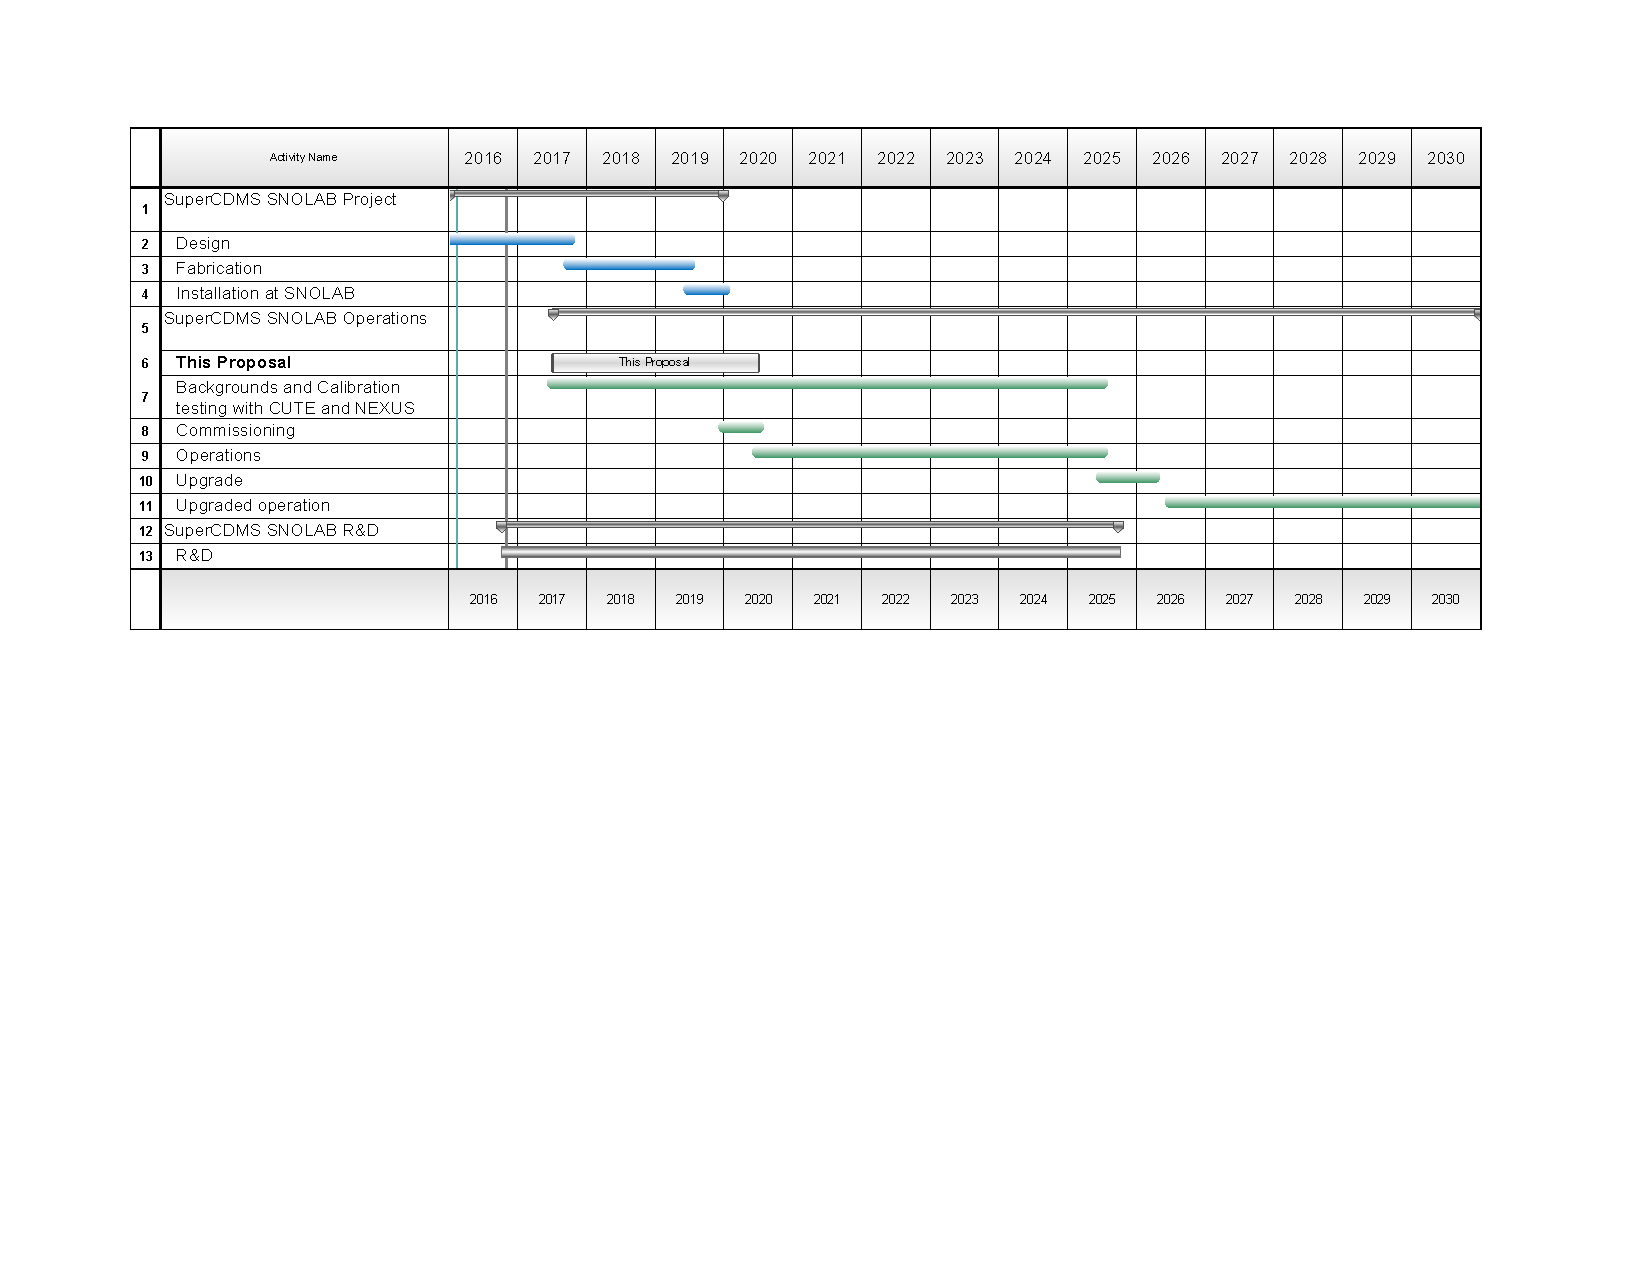
\includegraphics[width=\textwidth]{Figures/supercdms_operations_schedule_nsf_ops.pdf}
% \end{center}
% \caption{\footnotesize First draft of an interleaved schedule for the \scs Project, Operations and R$\&$D and Upgrades.}
% \label{fig:proj-schedule}
% \end{figure}

\begin{figure}[htb]
\begin{center}
  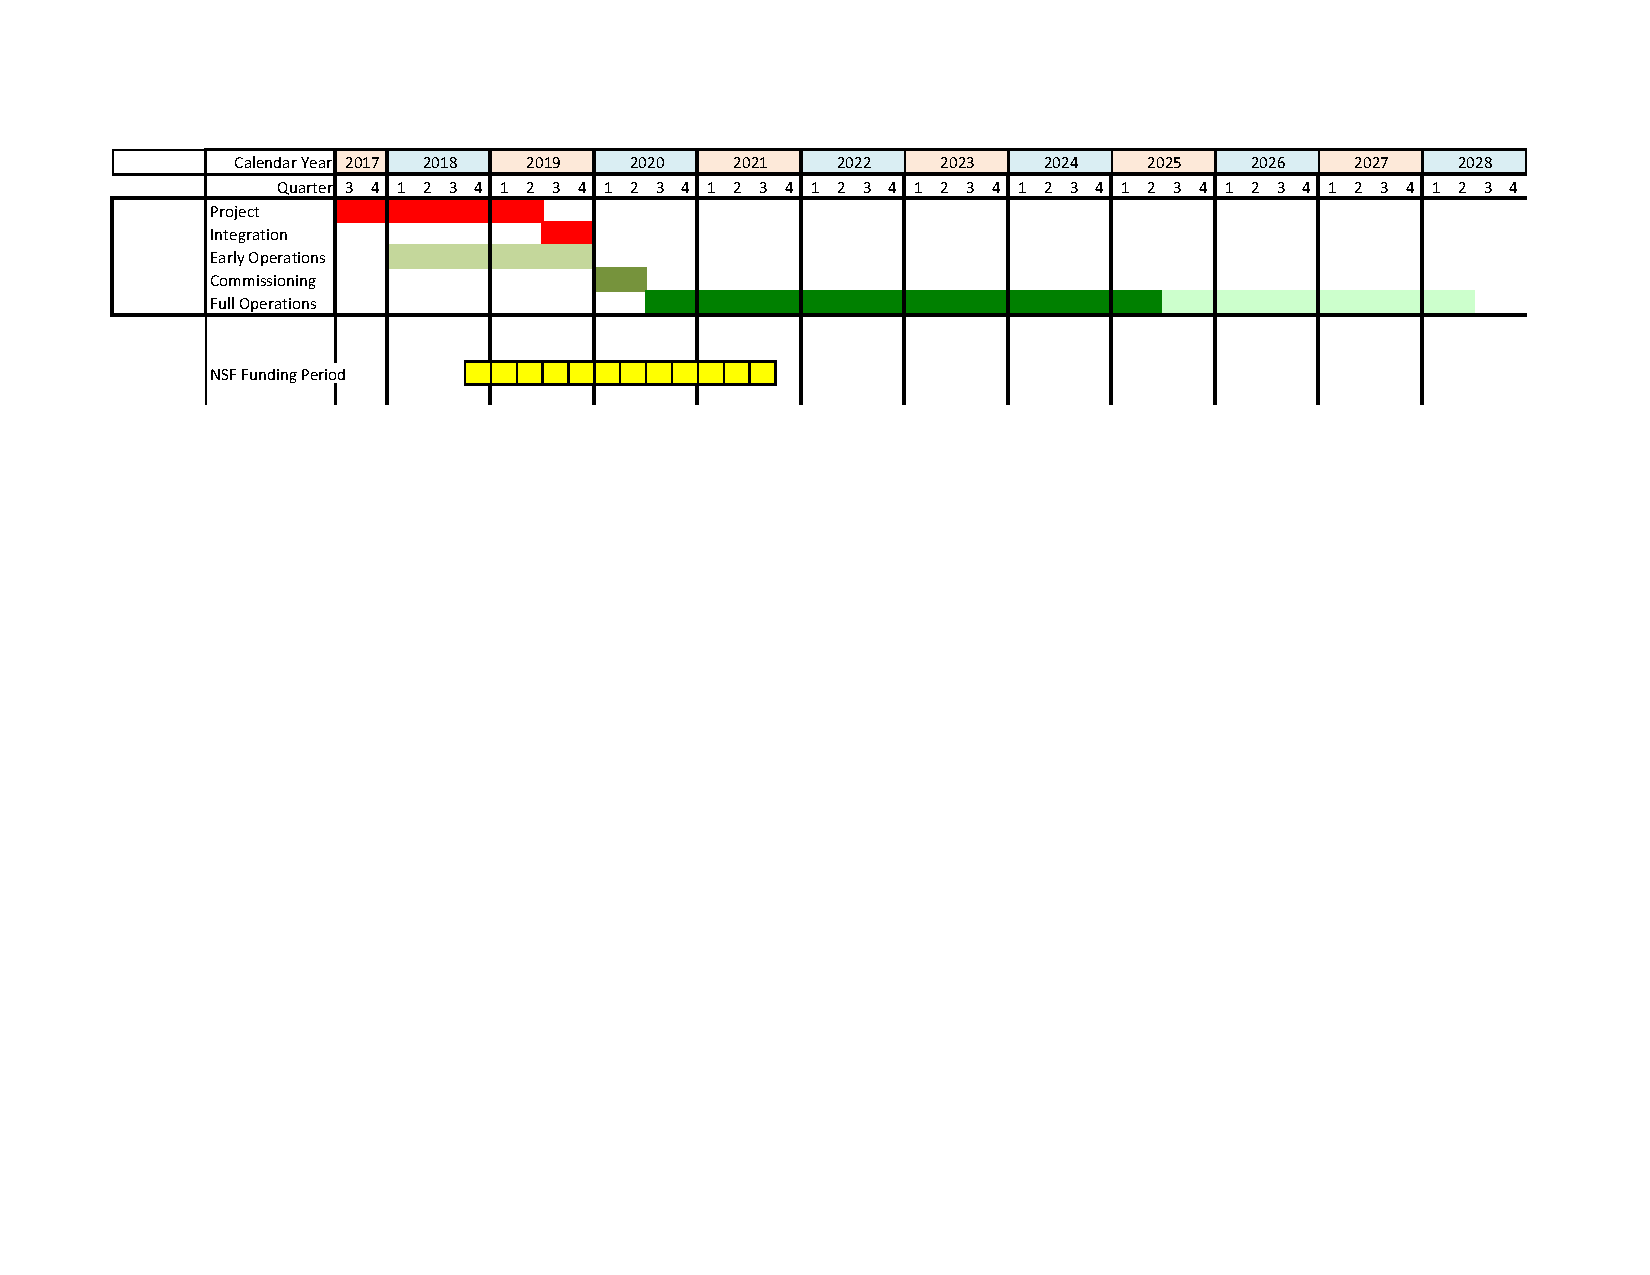
\includegraphics[width=\textwidth]{Figures/OpsSched-rac.pdf}
\end{center}
\caption{Schedule for the \scs Experiment.}
\label{fig:ops-schedule}
\end{figure}

\noindent\textbf{Year 1: 7/2018--6/2019}\\
During the first year the focus will be on calibration of the small HV test detectors from Stanford University with the Northwestern ADR at \tunl. These detectors will then be taken to \nexus, to perform cross-calibration measurements in preparation for the large detector calibrations. The first pre-production detectors arrive at \cute in January 2018, and the performance  and background measurement campaign begins soon after. 

\noindent\textbf{Year 2: 7/2019--6/2020}\\
The second year is dominated by runs of pre-production detectors at \nexus for calibration and at \cute for performance testing and background measurements. The first production \scs HV tower arrives at \cute in 12/2018, with testing commencing in 1/2019. Performance and run optimization of all six detectors of the HV tower will continue until 6/2020.

 \noindent\textbf{Year 3: 7/2020--6/2021}\\
There is no activity planned for \nexus on this grant in the third year. At \cute, the \scs HV tower science run will be taking data until 11/2019, when the tower will be taken out of \cute to prepare it for installation in the \scs experiment. Commissioning activities for \scs will be the main focus of this grant in the last six months of the award, along with the collaboration-wide effort in analysis and publication of all the data products from this work.

%\clearpage

% !TEX root = NSF_SuperCDMS_SNOLAB_OPS.tex
\section{Management}
\label{sec:management}
% RASCI chart?
% SWOT analysis?
% https://www.wrike.com/workspace.htm?acc=2707966#path=folder&id=335439022&a=2707966&c=timeline3&so=10&bso=10&sd=0&st=nt-1
% https://prod.teamgantt.com/gantt/schedule/?ids=1562286#&ids=1562286&user=&custom=&company=&hide_completed=false&date_filter=&color_filter=
% https://instagantt.com/r#

The management team of this NSF collaborative proposal will be chaired by the Northwestern PI and consist of all the PI's and Co-PI's of the proposal.  They will interact with the \nexus, \cute, and \SNOLAB facility managers to coordinate all the activities delineated in this proposal, as well as with the \SuperCDMS Collaboration for science analyses and training of students and postdocs.

The work funded by this proposal is part of the full set of \scs operations and commissioning activities, some of which are outside the scope of this proposal and are funded by DOE or Canadian funds. The management team for this proposal will be in close coordination with all parties involved in the \scs Project and Operations, as well as R\&D, and other \SuperCDMS Collaboration activities. These multi-agency collaboration-wide activities will be coordinated by a team consisting of the SuperCDMS SNOLAB Project and Operations Managers, the SuperCDMS Spokesperson, and the NSF Operations PI. This team will meet regularly to coordinate activities. 

The early operations phase of the \scs experiment covered by this proposal is when it is both necessary and appropriate to ramp up the operations management and support functions for \scs, which should all be in place for the commissioning phase of the experiment in order to ensure a smooth transition to the operations phase as quickly as possible.
%We are including a 10\% risk management overhead for the commissioning part of the proposal, as the success of commissioning will directly affect the much larger \scs Experiment. 

The detailed planning for commissioning of \scs will be led by a scientist identified to be the \scs Commissioner, with this role naturally evolving into that of a Run Coordinator during the operations phase. Details of the operations phase functions and management (which are outside the scope and period of performance of this project) are given in the \scs Experimental Operations Plan.
%Pre-operations and operations funding will be provided by DOE, NSF and NSERC/CFI. Therefore, during these phases, including commissioning of SuperCDMS SNOLAB, oversight will be provided by a Joint Oversight Group including the Program Managers from the agencies and other representatives of the DOE OHEP and NSF Physics Divisions as needed. The Operations Manager is appointed by the SLAC Director and Vice President for Research at Northwestern, with concurrence from the Fermilab and SNOLAB Directors, the DOE and NSF Program Managers, and the SuperCDMS Collaboration Spokesperson.   

%\subsection{Coordination between Operations and the Project}
%
%   There will be strong ties between the Project and Operations. The operations management will work together with the Project team to ensure that the experiment built by the project can be operated successfully and efficiently to deliver the science expected. The Project is completed upon installation of the experiment at SNOLAB. Commissioning and subsequent operation will be performed under SuperCDMS SNOLAB operations management. The pre-operations activities (mainly calibration and detector testing) that are outside the scope of the Project, but occurring at the same time as the Project, will be managed under the Operations organization, in close coordination with the Project.    
%
%Project Management and Operations Management will meet regularly to coordinate activities. Although operations activities are not part of the Project scope, some coordinated sharing of equipment and personnel can be expected. During the pre-operations phase, the Project will have the final decision on all equipment built with project funding and will have priority on use of technical personnel. The Project and Operations team will work together with the Collaboration management on sharing the effort of scientific personnel.   

\subsection{Facilities Management}
Since much of the work in this proposal occurs in dedicated underground facilities, we outline here the management of these facilities and their relationship to this grant's management.

\subsubsection{NEXUS}
The \nexus facility will receive primary management oversight from the Northwestern PI. In addition, \SuperCDMS collaborators at Fermilab will provide support to interface with Fermilab as needed. A fraction of an FTE will be provided by this grant for an operations manager, to oversee the activities delineated in this proposal. 

\subsubsection{CUTE}

The \cute facility will receive primary management oversight from our collaborators at Queen's University. This grant's management team will coordinate with Queen's to oversee the \cute activities delineated in this proposal.

\subsubsection{SNOLAB}

As mentioned above, the commissioning of \scs is an activity coordinated at the collaboration level. The PI of this grant will be part of the Operations Management team and will work closely with the \scs Operations Manager to coordinate and integrate the NSF-sponsored commissioning work with the overall multi-agency commissioning effort. \SNOLAB conducts a Gateway review process for projects which includes pre-operations activities, operation of the experiment, and decommissioning. For Gateway 1 and 2, the Project Director is the primary contact for review of the design and fabrication of the \scs experiment. For Gateway 3 and 4, the Operations Manager is the primary contact for review of the experiment pre-operations and operations. The Collaboration Canadian PI is involved in all interfaces between \scs project and operations and \SNOLAB management.  This grant's PI will be in close coordination with the Project Director, the Operations Manager and the Canadian PI to oversee the commissioning activities supported by this proposal.

%\subsection{Roles and Responsibilities of Funding Agencies}
%
%The \scs G2 Project is being jointly funded by DOE, NSF and CFI. While the scope of responsibilities for each funding agency has been carefully defined for the Project, we expect that all of these funding agencies will contribute to operating the \scs experiment, with additional research support from NSERC for Canadian researchers.  
%
%The DOE contributions to experimental operations will be managed through the SLAC National Accelerator Laboratory. The operations management office will be located there, that will report to a DOE-NSF Joint Oversight Group (JOG).


%
%\subsection{Interfaces between Operations and the Project}
%\label{sec:interfaces}
%There is obviously a strong tie between SuperCDMS Operations and the SuperCDMS SNOLAB Project, whose goal is to build the experimental facility and initial detector payload. The operations team will work together with the project team to ensure that what is built by the project will deliver the science expected. The Project is completed upon installation of the apparatus at SNOLAB. Commissioning and operation for the experiment will be handled under the SuperCDMS Operations management.
%
%There will be pre-operations activities (mainly calibration and detector testing) that are outside the scope of the Project, but occurring during the same time scale as the Project. These will be managed by the Operations organization. 
%
%\subsubsection{Management Coordination}
%The Project Management team and the Operations team will need to meet regularly to coordinate activities. By design, the operations activities are not part of the Project scope, but there may be conflicts over use of equipment or personnel. During the pre-operations phase, the Project will have the final decision on all equipment built with project funding and will have priority on use of technical personnel. The Project and Operations team will work together with the Collaboration management on sharing the effort of scientific personnel. 
%
%\subsubsection{Subsystem Management and Operations Leads}
%During the pre-operations phase, the L2 and L3 subsystem manager roles for the Project will be distinct from the Operations roles. As the Project nears completion, the Project and Operations management will discuss how best to merge expertise from the Project into Operations roles.
%
%\subsubsection{Reviews and Working Meetings}
%Project management will be invited to operations reviews and operations working meetings during the course of the Project. Similarly, operations management will be invited to project reviews and project working meetings.
%
%\subsubsection{R$\&$D}
%The collaboration will be conducting R$\&$D outside of the scope of either Project or Operations. Project management and operations management will be kept informed of the scope and resource usage for these R$\&$D activities, and the progress and results from the R$\&$D efforts.
%
%\subsubsection{Interfaces with SNOLAB}
%SNOLAB conducts a Gateway review process that parallels the DOE CD process, but also incorporates pre-operations activities, operation of the experiment and decommissioning. The Project Director is the primary contact for contact for the design and fabrication of SuperCDMS SNOLAB during Gateway 1 and 2, and the Operations Manager is the primary contact for pre-operations and operations during Gateway 3 and 4. The Collaboration Canadian lead PI is involved in all aspects of SuperCDMS SNOLAB and will be included in all interfaces with SNOLAB management. 
%
%\clearpage

% !TEX root = NSF_SuperCDMS_SNOLAB_OPS.tex
\section{Broader Impacts}
\label{sec:broad}

The SuperCDMS collaboration continues to deliver on its potential for broader impact including strong technical development, education at all levels, and engaging public outreach.

\textbf{Technical Development}
CDMS and SuperCDMS have developed, and continue to advance detector technologies that have significant impact both inside and outside of the dark matter community. These technologies include electrothermal feedback, transition-edge sensors (TESs); detection and utilization of athermal phonons; large, kilogram-scale phonon-mediated germanium and silicon-based detectors; arrays of large-scale, low-noise SQUIDs; and usage of LPN HEMPTs for ionization readout.

The field of direct detection of dark matter has benefited from these advances. The EDELWEISS and CRESST collaborations have both implemented some of these concepts. In addition, SuperCDMS’ pioneering of very-low-mass WIMP detection has had a strong impact on the field. There are now many R\&D efforts focused on very-low-mass WIMP detection. Multiple of these programs are run by PIs who were primarily engaged in liquid noble direct detection. The concepts developed by SuperCDMS have had far reaching impacts benefiting even direct detection experiments using the liquid nobles. 

The broader, basic-science community has benefited from SuperCDMS technology advances. The TES technology is now a core technology for multiple cosmic microwave background experiments including APEX, South Pole Telescope, and PolarBear. It is being rapidly adapted for far-infrared instruments including Super-SCUBA, single-photon spectroscopy, and large X-ray calorimetry experiments at NIST and NASA GSFC including the forthcoming Micro-X, which will launch the first TES into space. In addition, the TES technology is beginning to impact industry as TESs are being adapted for use in electron microscope sensitive surface element analysis and are being investigated for use in quantum coherence and computing.

The direct impact of SuperCDMS research is underscored by the number of graduate students impacted and the number and quality of the SuperCDMS publications. In the past three years, SuperCDMS has produced 12 Ph.D. theses and 11 science publications not including conference proceedings. The impact of these publications is underscored by their many citations (over 3,000 since 2011).

\textbf{Undergraduate, Graduate, and Postgraduate Education}
Direct detection of dark matter is multidisciplinary and therefore creates a broad spectrum of opportunities for students to explore and advance in many fields. From year to year, numerous undergraduates, graduate students and postdoctoral researchers from the SuperCDMS NSF-funded institutions have benefited from these collaborative opportunities and have been guided to develop precise simulations of semiconductor-based detectors, sensitive analysis techniques, statistical applications, and application of advanced software techniques. These opportunities combined with regular mentoring have afforded many high-visibility talks for students and postdocs. 

As a collaboration, SuperCDMS strives to ensure that graduate students and postdoctoral researchers receive proper exposure to the wider dark matter and particle physics communities to support their scientific development and establish the basis for future career and collaborative opportunities. To that end, a committee within the collaboration, headed by a senior member, identifies and advocates for high profile talk opportunities within the dark matter field. PIs from institutions on this proposal have provided strong representation on this committee. Interactions between university-based scientists and technical experts in industry, particularly in the areas of cryogenics and electronics continue to provide long-term benefits to the physics community at large, and are likely to lead to excellent job opportunities for some of our students.

Over the past seven years, SuperCDMS grad students have attained postdoctoral appointments at Caltech, Stanford, MIT, UC Santa Barbara, Texas A\&M, Northwestern, NASA GSFC, MIT, Berkeley, Lincoln Labs, LBNL and Fermilab, and others are pursuing careers in industry and tech. Also in this period, grad students and postdoctoral researchers from SuperCDMS NSF-funded institutions have obtained faculty appointments at Caltech, UC Berkeley, U. Illinois at Urbana-Champaign, San Diego State U., U. Massachusetts-Amherst, and three are senior researchers at NIST, SNOLAB and PNNL. The current SuperCDMS analysis coordinator is from an NSF-funded institution. 

Broad engagement of undergraduates in the research continues to be a strong focus. Currently, there are more than 25 undergraduates involved in SuperCDMS research, gaining the direct lab experience that is increasingly a discriminator in graduate school admission and an important complement to the undergraduate, mostly theoretical, education. At Northwestern University, the PI participates in the Summer Research Opportunities Program, which brings students from other US institutions to Northwestern and other universities in the Big Ten Alliance. Of the 34 undergraduates he has supervised, 15 were female and 10 were members of an underrepresented minority. 

Colegio de Física Fundamental e Interdiciplinaria de las Ámericas (COFI) is a physics research institute in San Juan, Puerto Rico, which hosts summer schools in different topics in physics, for graduate and undergraduate students, as well as talks for public audiences. In Summer 2016, the topic was high-energy physics instrumentation, in which Northwestern University PI Figueroa-Feliciano participated. The Institute is interested in partnering with SuperCDMS to bring theorists and experimentalists to their summer schools to give talks on dark matter and related topics. COFI opens its summer schools to all students (undergraduate and graduate students), but has a particular mission of bridging the span between North America and South America, bringing students and researchers from South America to interact with US researchers in San Juan. Given its unique character as a Spanish-speaking location in the US, this is a natural bridge between the communities. COFI is also interested in reaching students from underrepresented groups and bringing them to their summer schools.  In year 2, SuperCDMS will provide two speakers on dark matter-related topics at a COFI summer school. 

At Berkeley, undergraduates will be largely drawn from subsidized campus programs, including the Undergraduate Research Apprenticeship Program (URAP) and CalTeach, a program that enables science majors to concurrently complete their BS degree and a California teaching credential. The Compass Project, an initiative developed by Berkeley physics graduate students and launched in August 2007, aims to increase the percentage of minority and women students that matriculate with a bachelors degree in one of the physical sciences by engaging students who express an interest in such fields as early as possible. As the program’s faculty advisor, Bernard Sadoulet has facilitated their efforts to ensure the sustainability of this proven recruitment and retention program, by helping them secure a long-term, institutionalized base of support. Compass received the 2012 Award for Improving Undergraduate Physics Education, by the American Physical Society. Compass offers an intensive summer program for incoming freshmen from underserved schools, fall and spring term retention courses (including a course for transfer students to support their transition to Berkeley), mentoring, a research lecture series, and other social and academic support. %(http://www.berkeleycompassproject.org/programs/physics-98/).

Sadoulet is the director of Berkeley Connect in Physics, a mentoring program within the physics department that accepts undergraduate students at all levels. The course is a small seminar class led by a physics graduate student, under the guidance of the director. The goals of the program are to help students develop understanding, community, and career preparedness that go beyond what traditional courses provide. Interactions with graduate students and faculty play a large role throughout the semester. Under Sadoulet’s leadership, this course has significantly gained in enrollment with every succeeding semester since its launch in Spring 2014. %(http://www.berkeleyconnect.berkeley.edu/physics/).

The Physics Department at CU~Denver maintains an undergraduate-only program committed to providing students with hands-on research experience at this urban campus. The Department operates in close collaboration with the Physics Department at Metropolitan State University of Denver, and students from both institutions participate in the CU~Denver group’s activities, broadening the reach of the research program beyond a single institution. Underrepresented groups and first-generation college students are well represented in the PI’s group, and many of his mentees have proceeded to graduate school in physics and other disciplines, or embarked on careers in industry at companies such as Northrop Grumman. Currently, there are eight undergraduates in the CU~Denver group majoring in Physics, Electrical Engineering, and Mechanical Engineering.  

At the U. Florida, the PI has been the Education Outreach contact person for the Physics Department. His group hosts three (non UF) undergraduates for summer research internships as part of the REU program. 

%The TAMU SuperCDMS group has four PIs who oversee the activities of four postdocs, eight graduate students, and more than six undergraduate students who contribute to the research, including detector fabrication and polishing efforts. 

Southern Methodist U. typically funds one to three undergraduate students to work with the Cooley group each year. In the past five years, the eight undergraduates who have participated in the group’s research have either entered graduate programs in physics or engineering or embarked on careers in industry at companies such as Texas Instruments and AT\&T.  

The PI at the U. South Dakota serves as the Chair of the SuperCDMS Outreach Committee, and is a member of the Education and Outreach committee at USD. He increases the opportunities for undergraduates at USD and other institutions by mentoring non-physics and physics undergraduates in their honors thesis. The PI has been instrumental in bringing new, popular physics demonstrations to life including a Ruben’s tube and a cloud chamber that are now used in introductory physics classes. He has recruited four undergraduates who have contributed to the PI’s research program in the past two years, and he has guided two undergraduates through the process of writing a proposal for a NASA Research Stipend. A major issue confronting many undergraduate physics majors from colleges and smaller universities is the lack of exposure to the many fields of physics research. To address this issue, the PI presents colloquia and seminars at local colleges and universities, helping to spread the word about the new USD PhD program. All domestic students accepted into the USD Fall 2015 graduate class were a direct result of the PI’s talks. The PI is attempting to strengthen undergraduate research opportunities at USD through partnership on two USD NSF REU proposals. The PI was an organizer of the 2015 NSF sponsored USD Germanium Workshop and actively sought to increase minority and female participation at the workshop. As a result, 23\% of the participants were women, 80\% of whom were presenters. The PI personally invited one third of the minority attendees and arranged for all of them to give plenary talks. 
In addition to engaging undergraduates on campus, SuperCDMS will support an 8-week undergraduate summer research internship at SNOLAB, in years 2 and 3.

\textbf{K-12 Education}
SuperCDMS institutions provide strong support for K-12 education through programs for both teachers and students. Too numerous to describe in detail in this proposal, these programs take place in local schools, on campus and directly in the lab. At the core of many of the programs is engagement of students from disadvantaged backgrounds and underrepresented groups, including women. 

CU Denver, U. Florida, SMU, and USD engage middle school students in physics learning through lab tours, classroom visits and science camp. Northwestern U., UC Berkeley, U.~Florida, TAMU, SMU, and SD School of Mines and Technology support a range of high school programs, including summer research internships for students and teachers, hands-on research projects for underserved high school students of color, mini-courses to prepare Native American students for postsecondary education in science and engineering, interviews with physicists conducted by high school students, and structured physics courses for high school teachers. 

\textbf{Local Public Outreach}
SuperCDMS groups are actively engaged in efforts to share SuperCDMS science with the public. PIs and group members at Northwestern, UC Berkeley, and CU Denver present public lectures on dark matter, on campus, at community events and civic organizations, and at science cafes. The PI at Northwestern has presented two talks in the past year in San Juan, Puerto Rico. 

UC Berkeley, U. Florida, SMU, SD School of Mines and Technology, and TAMU participate in outreach events on campus, at community festivals, local farmers’ markets, science fairs and science camps. Activities include lab tours and hands-on physics demonstrations. SuperCDMS scientists have been featured in the media, including NPR’s Science Friday and in the popular press. 

\textbf{Site-Based SuperCDMS Education \& Outreach}
In recent years, SuperCDMS has taken advantage of the Soudan Underground Laboratory’s (SUL) location in a state park to impact thousands of tourists and dozens of school groups each year through laboratory science tours. These tours have taken students and tourists 2,341ft below the surface to the underground laboratory to view the SuperCDMS and MINOS experiments. At a SuperCDMS interactive table on the tours, tourists and students had the opportunity to not just see and hear about the SuperCDMS experiment but also physically interact with experimental elements including a sample detector. In addition, SuperCDMS scientists would speak directly with the public at a full-day science Open House, which attracted around 600 people annually. At the surface, a touch-screen kiosk continues to provide videos and descriptions of the SuperCDMS (and MINOS) experiments. 

With the departure of SuperCDMS from SUL and the completion of MINOS, underground outreach activities have ceased. However, the Ash River SUL group, under the leadership of Prof. Richard Gran (U. Minnesota-Duluth) is continuing outreach activities at a nearby NOvA site, with plans for a NOvA-centric summer program. The SUL Outreach Education Coordinator reports that public audiences and science educators are intensely interested in SuperCDMS science, and staying current with SuperCDMS SNOLAB is a priority. SuperCDMS will team with the Ash River SUL group (see the attached letter of collaboration) as a perfect conduit to continue our SUL Minnesota outreach. We will provide the Ash River SUL group SuperCDMS support and materials including posters, and virtual tours focused on the history of dark matter and neutrino physics. SuperCDMS will also enable the NOvA SUL group to effectively speak about dark matter by continuing to develop answers to commonly asked dark matter questions.

SuperCDMS is already reaching out to the public at the future experimental site, SNOLAB, and envisions growing that outreach during the timescale of this proposal to a level similar to the Soudan outreach. SuperCDMS is currently engaging SNOLAB tour groups by displaying a poster at a regular tour stop in the underground lab. In addition, SuperCDMS is highlighted in the SNOLAB “NewEyes on the Universe,” an interactive, mobile exhibit, which debuted in London, England, in July 2016.

SuperCDMS’s SNOLAB education and outreach will ramp up on a timescale parallel to its operational ramp. SuperCDMS will increase the impact on underground tours by developing an interactive display that enables tour members to explore the question of dark matter and the SuperCDMS experiment. SNOLAB has developed an online virtual tour that enables the general public to tour the SNOLAB underground lab remotely, be it from home, school, museum or community center. 

The “Ladder Labs” area, which will house SuperCDMS, is already featured in the virtual tour. SuperCDMS will explore ways to strengthen its engagement with virtual tourists including virtual science “treasure hunts.” These hunts will be designed to tell the science stories behind SuperCDMS’s search for dark matter. For example, one hunt will follow the life story of a dark matter detector as it is built at TAMU, tested at Berkeley, and installed at SNOLAB. Another will tell the story of the importance of eliminating radioactive backgrounds and how the SMU and SDM\&T groups are helping to solve this problem for SNOLAB. These virtual tours will be augmented by a web presence and social media platforms, making the science compelling and accessible to teachers, students and the general public.

We will coordinate our outreach efforts with the SNOLAB education and outreach team to leverage resources. For example, each year, high school students enroll in the International Summer School for Young Physicists. The students spend part of their time on underground science tours at SNOLAB. SuperCDMS graduate students and postdocs will serve as science guides for these students during the time underground. Each summer, the Tri-Institute Summer School on Elementary Particles (TRISEP) is held at Laurentian University in Sudbury. We will participate by sending graduate students to TRISEP and offering SuperCDMS faculty to serve as TRISEP educators. 

The 2017 TAUP conference will be held in Sudbury, and we anticipate using TAUP as a launching point for faculty and student involvement at SNOLAB. In addition, we will participate in SNOLAB education and outreach programs as opportunities arise and will provide outreach materials to SNOLAB.

SuperCDMS will broaden its scope of outreach to also include the Sanford Underground Research Facility (SURF). At SURF, the USD and SDSM\&T PIs are working with the SURF E\&O team to coordinate an outreach program beginning with a presence at SURF Neutrino Day. Neutrino Day is an annual outreach event at SURF that has live science demonstrations and talks that directly reaches about 1,000 people and indirectly reaches tens of thousands through resulting media coverage including a live South Dakota Public Radio broadcast.

In addition, we will develop six dark matter education modules for integration of SuperCDMS science into the SURF “Search for Dark Matter” middle school curriculum. These units are designed to aid teachers in the classroom and fill a South Dakota educational requirement. It is part of SURF’s strategic plan to expand these beyond South Dakota. The Berkeley group will look into how three of these modules can be modified to accommodate California educational standards, and the Northwestern U. group is willing to host three of these modules for use by educators in the Chicagoland area. We will support a SURF education person to travel to Sudbury to provide teachers with a 2 to 3 day professional development workshop on the implementation of the curriculum materials. 

Another priority is to establish an alliance with Sudbury's First Nations communities for the sharing of science education. This is of interest to the outreach division at SNOLAB, and SuperCDMS has already expressed interest in working with them on development. CDMS at Berkeley has experience in this area through an established association with the founder and leadership team of the Native American Science Academy. Through this alliance, SuperCDMS will also develop channels to integrate SuperCDMS science with indigenous science education in the US.


%\clearpage

% !TEX root = NSF_SuperCDMS_SNOLAB_OPS.tex

\section{Results from Prior NSF Support}
\label{sec:prev-res}

In this section we describe the results from prior NSF support, divided by institution. Note that Co-PI J.~Sander has not recieved NSF Funding in the last 5 years, and that Co-PI M.~Pyle was funded through a Berkeley award as a postdoctoral researcher.

\subsection{Northwestern University, PI E. Figueroa-Feliciano}

\vspace{3pt}
\noindent\textbf{PHY-1408089, PHY-1550658}\\ 
\emph{Dark Matter and Neutrino Physics with Cryogenic Detectors}\\
Period of Support: 7/2014--8/2017, transferred from MIT to Northwestern as PHY-1550658 when Figueroa-Feliciano moved to Northwestern. Amount of Support: \$330,535\\
Publications:~\cite{SuperCDMSSensitvitiy:2016arXiv,Agnese:2015nto,OHare2015Readout-strateg,Agnese:2015ywx,Schneck2015Dark-matter-eff,Pyle2015Optimized-Desig,Agnese:2014xye,Agnese:2014vxh,2015PhRvD..91i5023B,Ruppin:2014bra,Agnese:2014aze}\\
Data products from this work are available at the \SuperCDMS collaboration's publications website~\cite{CDMSpubs} and the Figueroa group's website~\cite{FigueroaWeb}.


\subsubsection{Intellectual merit} 
This grant supports students and scientists working on an experiment that will address one of the most fundamental problems of modern science, the nature of dark matter. The \scs experiment will achieve world-leading sensitivity for dark matter searches in the 1--10~\gev mass range.

Analyses of CDMS~II data demonstrated the power of improved analysis techniques~\cite{Agnese:2014xye,Agnese:2015ywx}, and provided limits for alternate dark matter models~\cite{Agnese:2014vxh}. It also revealed a possible signal on Si~\cite{Agnese:13prl}, the analysis and publication of which was lead by the Figueroa Group, then at MIT. 
Operation of 15 \SuperCDMS ``iZIP'' detectors at Soudan since 2012 demonstrated the detectors' rejection capabilities~\cite{Agnese:13apl} and yielded world-leading sensitivity to low-mass 
DM~\cite{Agnese:13prl2,Agnese:2014aze,Agnese:2015nto}.  Our group designed the masks used to fabricate the detectors in \SuperCDMS Soudan, had major roles in the rejection capability analysis, and led the low-treshold analysis \cite{Agnese:2014aze} from \\SuperCDMS\ \Soudan.
The first operation of a single (``CDMSlite") detector with a high voltage bias provided the world's most constraining limits for DM masses below 6\,GeV$/c^2$ by achieving an extremely low energy threshold of 170\,eV electron-recoil energy~\cite{Agnese:13prl2}. A second run of the detector reached an energy threshold for electron recoils as low as 56\,eV and demonstrated the power of a fiducialization cut~\cite{Agnese:2015nto}. The Figueroa Group developed key data quality cuts for the first two CDMSlite run analyses, and is currently involved in the analysis of the third run.
 
The Figueroa Group made the first map of the so-called ``neutrino floor" in the WIMP-nucleon cross section vs WIMP mass plane~\cite{Billard:14prd}. As part of this grant the group has expanded this work to study complementarity and the effect of target on the neutrino floor~\cite{Ruppin:2014bra}, and contributed to a study on moving beyond the neutrino floor with directional detection~\cite{OHare2015Readout-strateg}. We also looked at the prospects of neutrino physics with dark matter searches~\cite{2015PhRvD..91i5023B}.
 
On the R\&D effort, the Figueroa Group has continued studying the active veto concept. As part of this grant, they developed a \geant Monte Carlo of both a bucket scintillator and Ge ring veto concepts.  They also made a design of a CDMS holder that will enable a test of a ring veto in a standard CDMS~II tower. Another R\&D effort has focused on the preparation of the ADR cryogenic system that will be made available for use for the \tunl calibration campaign described in Section~\ref{sec:tunl}. In addition, the Northwestern group has collaborated with the UF and Fermilab groups in the studies and simulations leading to the optimization and design of the calibration campaign described in this proposal.

\subsubsection{Broader impacts}
This grant strongly contributes to the training of undergraduate and graduate students and postdoctoral researchers, continuing the group's strong involvement in mentoring undergraduates from underrepresented groups by participating in the Summer Research Opportunities Program (SROP), which brings undergraduates from across the U.S. to do a summer of research at Northwestern. The group is also working to develop summer schools for training graduate students and postdocs at the ``Colegio de F\'{\i}sica Fundamental e Interdiciplinaria de las Americas" (COFI), located in San Juan, Puerto Rico.

\subsection{UC Berkeley, PI B. Sadoulet}

We summarize here the scientific and broader impact results obtained with NSF support at Berkeley over the past five years. Our group has been supported by awards PHY-1102841 (Jul 1, 2011-Jun 30, 2014, \$1,260,000, Experimental Particle Cosmology), and  PHY-1408597 (Aug 15, 2014- Jul 31 2017, \$1,177,400, Experimental Particle Cosmology). \SuperCDMS Soudan has been supported  by the NSF project award PHY-0902182 (Jul 1, 2010-Jun 30, 2013, \SuperCDMS Soudan, \$1,833,707) and operation award PHY-1004714 (Oct 2011-Sept 2013, \SuperCDMS Operation at Soudan, \$1,154,213) with UC Berkeley as the lead institution (PI B. Sadoulet) and subcontracts to MIT,  Santa Clara U., Syracuse U., U. Colorado-Denver, U. Florida, and U. Minnesota-Duluth. In addition, Berkeley (PI B. Sadoulet) has been the lead  NSF institution for the R\&D toward \SuperCDMS at SNOLAB (PHY-1242645, Sep 1, 2012- Aug 31, 2014, R\&D toward \SuperCDMS at SNOLAB, \$2,912,376) with subcontracts to MIT, Santa Clara U., and U. Colorado-Denver. Currently, Berkeley (PI B. Sadoulet) is the NSF lead institution of the \scs project (PHY-1415388, May 1, 2015-Apr 30, 2019, \scs, \$12,000,000) with subcontracts to Santa Clara U., U. Colorado-Denver, Stanford and SLAC, Texas A\&M, and U. of Minnesota-Twin Cities.

\subsubsection{Intellectual Merit}
\textbf{\SuperCDMS Soudan Science}

Over the past five years, \SuperCDMS Soudan has led the field in the search for low mass DM ($<$10 GeV/c$^{2}$) \cite{Agnese:2015nto,Agnese:2014aze,Agnese:13prl2}. Berkeley's contributions to this science output are delineated below:


\begin{compactitem}
	\item All prototype testing of the SuperCDMS Soudan iZIP for performance as well as the functional testing of every iZIP detector operated at Soudan was done in the Berkeley test facility.  
	\item Matt Pyle personally designed, tested, and optimized the SuperCDMS iZIP and 3 earlier generation prototype devices as part of his dissertation work  \cite{Pyle:12phd}. Fiducialization cuts used in \cite{Agnese:2015nto,Agnese:2014aze} were largely based on this work.
	\item Bruno Serfass led the  analysis effort during detector commissioning at Soudan and coordinates the collaboration wide software and computing group.
	% which was responsible for data processing and storage as well as the implementation of new algorithms .
%	\item The analysis effort during detector commissioning at Soudan was led by Bruno Serfass.
%	\item The Software and Computing Group which was responsible for data processing and storage as well as the implementation of new algorithms was led by Bruno Serfass. 
	\item Berkeley graduate student Todd Doughty led the underground ER/NR discrimination studies \cite{Agnese:13apl} as well as the SuperCDMS Soudan high mass dark matter analysis (to be published soon). 
	\item Berkeley led the optimization of the hardware trigger bandwidth for slower athermal phonon collection of the iZIP %due to sparse Al coverage
	 that decreased the energy threshold in our low energy analysis \cite{Agnese:2015nto}.
\end{compactitem}

\subsubsection{SuperCDMS SNOLAB Detector and Electronics R\&D}
\label{subsec:DetElRnD}
\begin{compactitem}
	\item Berkeley developed  complex impedance based techniques to distinguish the coupling mechanisms of the cryocooler noise at Soudan. Furthermore, via active measurement of the vibrational sensitivity of current athermal phonon detector technology, it has developed a vibrational specification for the SuperCDMS SNOLAB facility.

		
	\item %Charge Leakage Studies
	Dark current as a function of voltage bias has been measured for 5 test detectors at the Berkeley test facility. With this data, IR production and surface tunneling hypotheses have been disfavored.
	
	\item %Sensitivity Studies:
	The Berkeley group developed analytical detector modeling and sensitivity code for both the SuperCDMS iZIP and HV detectors that was used throughout the SuperCDMS design process (Fig. \ref{fig:SIdataProjections}) and which has recently been submitted for publication \cite{Agnese:2016cpb}.  A major upgrade to these sensitivity estimates, which is complete and soon to be published, models the quantization of ionization production which could potentially be used for ER/NR discrimination.
\item %Automation of Detector Testing:
	In CDMS-II and SuperCDMS Soudan, the labor associated with manual  testing of a detector was substantial. %has been a substantial fraction of the total detector cost. 
	As such, the SuperCDMS project has highlighted full automation of detector testing as a priority.  The Berkeley group has written semi-automated SQUID biasing and TES tuning routines %which interface with the SuperCDMS SNOLAB DAQ and warm electronics, 
	and a fully automated version should be operational in FY17. 
	
	\item %HEMT Charge Amplifier
	The SuperCDMS SNOLAB iZIP low mass sensitivity is largely determined by electronic noise in the ionization signal readout amplifier. In recent years, our collaborators at CNRS/LPN have developed low-noise, low-power high electron mobility transistors (HEMTs) with better low frequency noise performance than can be achieved with Si based JFETs. Berkeley has designed and built a HEMT-based charge amplifier located entirely at 4K to minimize the susceptibility to environmental noise pickup. HEMT switches have also been implemented to allow for the removal of the feedback resistor. 
	%without the noise of a feedback resistor. The  small spatial extent to minimize environmental noise pickups for a long  feedback loop to room temperatiure.
%	with a theoretical ionization resolution of 70 eV$_{ee}$ (300 pf input capacitance)
%	 that should also have reduced susceptibility to environmental noise due to the close proximity to the detector of all of it's components. 
We obtained a r.m.s. of  91 eV$_{ee}$ %, compared to a theoretical estimate of 70 eV$_{ee}$,
which exceeds the SuperCDMS SNOLAB goal requirement. The HEMT switch is currently under study for possible inclusion in the project baseline.
	%Substantial portions of this design are now being incorporated into the SuperCDMS SNOLAB charge amplifier designed under development by SLAC.  Berkeley is responsible for procuring HEMTs for the SuperCDMS SNOLAB Project
		
\end{compactitem}

%\subsection{\SuperCDMS Project}
\subsubsection{Broader Impacts}
Since 2004, the Berkeley group has partnered with the Level Playing Field Institute
to support the Summer Math and Science Honors (SMASH) Academy, an
enrichment program for high-achieving students of color from underserved Bay Area communities.
The group hosts a course for the incoming SMASH cohort, which engages them in research projects with
STEM grad students, many of whom are from underrepresented groups. 
The Berkeley group participates regularly
in campus and community-based outreach activities, described in more detail in Section 6.3 and is involved in the collaboration based outreach at Soudan.
%By virtue of being associated with a State Park, the Soudan Underground Laboratory has afforded
%CDMS particular access to public outreach through underground lab tours, which accommodate
%thousands of summer tourists and numerous school groups. The Lab has provided unique training
%opportunities for high school teachers, including development of related curriculum materials for
%primary and secondary school students, and undergraduate research internships. %The Soudan Education and Public Outreach program has been supported by PHY-1004714 (Oct 2011-Sept 2013, \SuperCDMS Soudan Operations, \$1,154,213) and currently by PHY-1212342 (Apr 2012-Mar 2015, Education and Public Outreach at the Soudan Underground Facility, \$267.823).

%\clearpage




\subsection{CU Denver, PI M. Huber}

%We describe here the scientific and broader impact results obtained with NSF support initiated within the past five years. In this time, the CU~Denver group has been supported by two direct awards and several sub-awards through UC Berkeley, the CDMS collaboration's lead NSF institution. 

The direct awards to CU Denver are NSF/PHY-1102795, ``SQUID-based Readout Systems for Cryogenic Dark Matter Detectors'' (\$163,711, July 1, 2011-June 30, 2015), and NSF/PHY-1408414, ``Readout Systems for Cryogenic Dark Matter Detectors'' (\$148,893, September 15, 2014-August 31, 2017). This work has resulted in publications~\cite{Agnese:13prl,Agnese:13apl,Agnese:13prl2,Agnese:2014aze,Agnese:2014vxh,Agnese:2014xye,Agnese:2015nto,Agnese:2015ywx}.
%Technical results of research and development towards (and beyond) \scs are described in Section~\ref{CUDenverResults}. Section~\ref{priorBI} describes the broader impacts of this prior NSF support.

%\smallskip
%
%
%\subsubsection{Intellectual Merit: \SuperCDMS Soudan Science}
%\label{CDMSresults}
%
%Analyses of CDMS~II data demonstrated the power of improved analysis techniques~\cite{Agnese:2014xye,Agnese:2015ywx}, revealed a possible signal on Si~\cite{Agnese:13prl}, and provided limits for alternate dark matter models~\cite{Agnese:2014vxh}. Operation of 15 \SuperCDMS ``iZIP'' detectors at Soudan since 2012 demonstrated the detectors' rejection capabilities~\cite{Agnese:13apl} and yielded world-leading sensitivity to low-mass DM~\cite{Agnese:13prl2,Agnese:2014aze,Agnese:2015nto}.  The results are in tension with WIMP DM interpretations of recent experiments~\cite{Agnese:13prl} and exclude the DM interpretation of the excess reported by the CoGeNT experiment, which uses the same target material (Ge), making comparisons between the results independent of theoretical uncertainties. First operation of a single (``CDMSlite") detector with a high voltage bias provided the world's most constraining limits for DM masses below 6\,GeV$/c^2$ by achieving an extremely low energy threshold of 170\,eV electron-recoil energy~\cite{Agnese:13prl2}. A second run of the detector reached an energy threshold for electron recoils as low as 56\,eV and demonstrated the power of a fiducialization cut~\cite{Agnese:2015nto}.
%
%
%\smallskip
%

\subsubsection{Intellectual Merit}
\label{CUDenverResults}

The CU~Denver group has played a prominent role in all aspects of the phonon readout system, utilizing the PI's extensive experience in SQUID design, characterization, and room-temperature electronics. The group supported operation of the \SuperCDMS Soudan facility through it's decomissioning, conducted research and development toward the \scs experiment, and pursued \RnD\ avenues with a view of improving detector readout for future CDMS programs. The group supports undergraduate education through extensive participation by Physics and Electrical Engineering majors in its various activities.

A primary activity of CU~Denver has been the evaluation of Superconducting Quantum Interference Device (\SQUID) series array preamplifiers. The microfabricated \SQUIDs\ are a key component of the phonon readout system. The CU~Denver group has advanced understanding of the requirements for phonon readout systems for the iZIP and HV detectors.  In collaboration with NIST-Boulder, work by the CU~Denver team contributed to the design of the next-generation SQUID array amplifier readout prototype. Intensive study of these prototypes, including measurement of the input self-inductance, dynamic resistance, equivalent input current noise, and closed-loop circuit bandwidth, allowed for a selection of the final design for the engineering detector tower. Precision measurement of the self inductances of the input and feedback coils, the mutual inductance between input and feedback coils, and the mutual inductance of each coil to the \SQUID\ fed into a model of the equivalent circuit of the TES + \SQUID\ system. Knowledge of these inductances informed design of the cold electronics striplines and connectors, by way of determining allowable levels of parasitic inductances on the input circuit. The resulting model and transfer function enabled simulation of the warm and cold electronics phonon readout system, which was essential in design of the warm-electronics circuit. These prototype tests also resulted in statistics for quantitative characteristics, qualitative metrics, and fabrication yield information. This process led to a standardized reporting format for characterizing the engineering-grade devices. To date, CU~Denver has tested all of  the $\sim$100 devices required for the Detector Tower engineering model and associated work at collaboration test facilities. The characterization has included the dc transfer function, ac (noise) performance, and measurement of other parameters of the \SQUID\ arrays.


%The CU~Denver group developed the high-volume \SQUID\ testing protocol required to meet the delivery schedule for production. The resulting infrastructure consists cryostat for measuring four devices in a single run, custom-made by the group, and electronics and software to gather the data at high resolution in an automated process.


CU~Denver has participated in the continued development of room-temperature electronics for \SQUID\ and TES readout. This participation has included measurements on the bench and with cold \SQUIDs\ of the performance of the warm electronics. These tests contributed to further development by FNAL of the Detector Control and Readout Card (DCRC) for \scs. From the testing of the prototype DCRCs, the CU~Denver group found that the noise levels and bandwidth are acceptable only if used with passive filtering. This and other testing informed the design of further generations of the warm electronics. With the FNAL and SLAC staff, the UC Denver group evaluated the schematics and design for the next-generation DCRC, which was expanded to operate 12 phonon channels (compared to the four previously), requiring a significant redesign of the circuit. The proposed circuit was evaluated to ensure it meets the technical requirements of the experiment. As a part of this evaluation, a member of the UC Denver team traveled to UC Berkeley to assist in testing the noise performance of the DCRC.


CU~Denver began studies of compatibility of the \scs\ \SQUIDs\ for planned \SuperCDMS high-voltage operation, which could require voltages that are internal to the SQUID circuit for which the devices were not designed. These studies included testing and development of instrumentation for high-voltage tests, and measurement of the voltage limit beyond which breakdown in the SQUID chip occurs. These tests contributed to the decision by the collaboration to set these high voltages by floating all of the warm electronics associated with a given detector side, so that there would be no large potential differences on an individual \SQUID\ chip.


The CU~Denver group conducted extensive tests on the performance of the \scs\ \SQUID\ arrays in various shielding environments. This testing included use of a large external high-permeability shield, close-in nested cryoperm cans, a close-in aluminum can, and a Faraday cage around the test probe. Additionally tests were done on the effects of certain metals (nickel and copper) in the vicinity of the SQUIDs, to provide information on the use of these materials in the cold-hardware design. From the tests on magnetic shielding and SQUID sensitivity, at Soudan and in Denver, the CU~Denver group found that the SQUIDs used in Soudan are sensitive to ac magnetic fields with an amplitude ($\sim$0.7 mG) similar to ambient fields found at the experiment site. The \SNOLAB\ \SQUIDs, which have a different design, were found to be less sensitive ($\sim$1.9 mG) to magnetic noise pickup. The CU~Denver group also measured the stability at cryogenic temperatures of candidate shunt resistors to be used for the TES circuit in the detector towers.

The CU~Denver group investigated the feasibility of a SQUID-based charge-pulse readout for CDMS. The resonant frequencies of the coils of a superconducting transformer, which was fabricated by the group, were measured using a vector network analyzer. The work was concluded when the use of HEMTs for charge readout, rather than \SQUIDs, was chosen.

CU~Denver supported operation of \SuperCDMS Soudan through regular shifts at the experimental site in the Soudan Underground Laboratory. The PI and the Senior Engineer both served multiple on-site shifts at Soudan. 

\subsubsection{Broader impacts}
\label{priorBI}

%Previous grants from the NSF has supported students and scientists working on an experiment addressing one of the most fundamental problems of modern science, the nature of dark matter, in a way complementary to the Large Hadron Collider and indirect detection experiments. The \scs experiment has achieved world-leading sensitivity for dark matter searches in the 1--10~\gev mass range.

The CU~Denver Physics Department maintains an undergraduate-only program committed to providing students with hands-on research experience at this urban campus. Electrical Engineering and Mechanical Engineering students have also participated in internships in the CU~Denver lab. Minorities and first-generation college students have been well represented in these internships, and many of the PI's mentees have proceeded to graduate school in physics and other disciplines, or embarked on careers in industry at companies such as Northrop Grumman and the Lockheed Martin Corporation. In the preceding five years, there have continually been six to eight undergraduates in the Huber group. 

At CU~Denver, the PI has participated with a local magnet school, the Logan School for Creative Learning, in their field trip program. Students in grades 5 - 8 have participated in small group discussions with him on topics of interest to them in the field of physics, followed by a tour of the laboratory. Their conversations with Huber and their tours of the lab are key components of presentations they give to their classmates and other visitors during the school's annual EXPO event. Students from other local middle schools and high schools have also participated in the lab's activities.

The CU~Denver PI has presented public talks on dark matter and the CDMS experiment at institutional and other local venues, which have included the CU~Denver Mini-STEM School and the Denver Cafe Scientifique. He has a standing invitation to return for future talks at Cafe Scientifique. The CU~Denver senior engineer gave a talk to a local Rotary Club about the search for dark matter and CU~Denver's involvement, addressing about 100 business and cultural leaders of the communitiy.


\subsection{\SuperCDMS Collaboration Broader Impacts}
The \SuperCDMS experimental and R\&D efforts advance phonon-mediated detectors and new active veto concepts, which have already found many applications in cosmology, astronomy and industry. 
Collaboration wide, a priority is the education of the groups' undergraduate and graduate students and postdoctoral scholars, providing them with opportunities to explore and advance in many fields. The success of this emphasis is evidenced in the high level of professional advancement of these students and postdocs, to careers as faculty, research scientists and technology experts in industry. \SuperCDMS PIs participate in programs to support K-12 students and teachers in their local schools, on campus and directly in the lab. At the core of many of the programs is engagement of students from disadvantaged backgrounds and underrepresented groups, including women. These programs include summer research internships, a program engaging underserved high school students of color in research projects, mini-courses to prepare Native American students for postsecondary education in science and engineering, and structured courses in physics for high school teachers. SuperCDMS groups have actively engaged in efforts to share \SuperCDMS science with the public, through lectures on dark matter at diverse venues, including campus lecture halls, science cafes and civic organizations. The groups regularly participate in outreach events on campus, at community festivals, science fairs and science camps. Activities include lab tours and hands-on physics demonstrations. SuperCDMS scientists have been featured in the media, including NPR's Science Friday and in the popular press. 


\clearpage
\pagenumbering{arabic}
\addcontentsline{toc}{section}{\bf References}
\bibliographystyle{unsrt}
\bibliography{supercdms_references}

%% Does facilities & equipment need to be part
%% of the main body?
%\clearpage
%\pagenumbering{arabic}
%%!TEX root = NSF_SuperCDMS_SNOLAB_OPS.tex

%------------------------------------------------------------------
%------------------------------------------------------------------
\clearpage
\rhead{}
\setcounter{section}{0}
\noindent\textbf{\LARGE{Facilities, Equipment, and Other Resources}}\\


\documentclass[11pt]{article}
\usepackage{color}
\textwidth 6.5in
\textheight 9in
\topmargin -.50in
\oddsidemargin 0pt
%\linespread{2.0}
%\renewcommand{\topfraction}{0.5}
%\renewcommand{\bottomfraction}{0.5}
%\renewcommand{\textfraction}{0.1}


\setlength{\parindent}{0pt}
\setlength{\parskip}{1em}

\def\ni{\noindent}
\def\ss{\smallskip}
\def\ms{\medskip}
\def\bs{\bigskip}
\def\eg{{\it e.g.}}
\def\ie{{\it i.e.}}

\newcommand{\RnD}{{\small R\&D}}
\newcommand{\TES}{{\small TES}}
\newcommand{\SQUID}{{\small SQUID}}
\newcommand{\SQUIDs}{{\small SQUIDs}}
\newcommand{\UCD}{{\small UCD}}
\newcommand{\NIST}{{\small NIST}}
\newcommand{\NEXUS}{{\small NEXUS}}
\newcommand{\BMF}{{\small BMF}}
\newcommand{\SuperCDMS}{{\small SuperCDMS}}
\newcommand{\CDMS}{{\small CDMS}}
\newcommand{\SNOLAB}{{\small SNOLAB}}


\pagestyle{empty}
%\pagestyle{myheadings}%empty}%
%\markright{Budget Justification [\today]}

\begin{document}
%\onecolumn
%\pagenumbering{arabic}
%\setcounter{page}{25}


%\centerline{\bf Facilities, Equipment, and Other Resources}
%\centerline{\bf University of Colorado Denver}
\noindent
\section*{Facilities, Equipment, and Other Resources}

%\section*{University of Colorado Denver}

\bs
%\ni {\bf {\small FACILITIES:}}
\subsection*{\small FACILITIES:}
%\bs
{\bf Laboratory Facilities: }
The PI has dedicated laboratory space on the downtown campus of the University of Colorado Denver, near Physics faculty and staff offices and other Physics Department resources.  The PI's computational laboratory is 380 sq ft and provides  working space for at least six students.  Her lab includes an ADA-accessible ``telephone booth'' for group members who need to join remote meetings with collaborators.

%\bs
%\ni {\bf Clinical Facilities:}
%\ni N/A
%
%\bs
%\ni {\bf Animal Facilities:}
%\ni N/A

\bs
\ni {\bf Computer Facilities:}
Internet services (off-site as well as connections between the lab and offices) are maintained by the campus Information Technology Services, as are secure web servers for all aspects of the CU Denver campus operations, including research group activities. All offices and laboratories have ample network ports.

\ms\ni
In addition to these campus-level networking resources, the PI's laboratory has three workstations and three laptops available for student check-out.  The workstations are equipped with USB-C docking stations.  This setup allows students to work when and where they need and provides a convenient space for short conferences.  All of the available machines can be used for data analysis and data acquisition development.  All of the available machines have software and operating system support administered by the campus Information Technology Services.

\bs
\ni {\bf Office Facilities:}
\ni The PI is also provided with a private office with telephone and computer network connections. Other personnel will be quartered in laboratory offices as described above or in shared office spaces.

\bs
\ni {\bf Other Facilities:}
\ni
The PI has access to computing clusters at SLAC and gigabyte-scale dark matter data sets through her collaboration with SuperCDMS.  These resources are available for testing the analysis tools with large data sets.  The SLAC cluster is maintained by its local institution. 

%Both Roberts and Villano have active accounts on the clusters listed above and can request computational time for projects related to \CDMS.  In addition Villano will negotiate for time at the \NEXUS\ facility which will have neutron-source and cryogenic detector equipment available for the neutron-capture calibrations he is planning. 
%\bs
\subsection*{\small MAJOR EQUIPMENT:}

The PI does not have additional major equipment; no major equipment is needed for this proposal.

\bs
\subsection*{\small OTHER RESOURCES:}

\ni
{\bf Senior Personnel:} The PI anticipates hiring a professional research assistant (PRA) to work on implementing standards-based data analysis tools, writing supporting documentation and tests, and coordinating the developer side of the proposed community workshops.  %The Physics Department along with the College of Liberal Arts and Sciences commits additional time for the PRA to work on this proposal.

{\bf Administrative Support:}  The PI is provided with department-level support from a shared secretarial staff.  These staff manage time sheets and student pay and help manage travel and purchases.  In addition, the Office of Research Services supports faculty in research endeavors and have staff with expertise in conference and workshop design.   

{\bf Student Support:}  CU Denver students have 24/7 access to a food pantry that is stocked with non-perishable foods and sanitary products.  In addition, the CU Denver Career Center offers career services to both undergraduate and graduate students and uses the handshake platform extensively to match students with on-campus research opportunities.  The counselors at the Career Center are certified in [some kind of therapy thing] and serve as a complementary career-readiness resource to the PI.




%  Villano anticipates hiring a 1.0 FTE Postdoctoral Research Associate starting in Year 2 of the requested support.  The total support from this proposal, should it be fully funded, will result in 0.5 FTE in project Years 2 and 3.  

\end{document}







%\clearpage
%\rhead{}
%\rfoot{}
%
%\input{E-Facilities}
%\clearpage
%\input{G-Data_Management}
%\clearpage
%\input{H-Mentoring}

\end{document}
